% enable this to activate the version for PRINT
% disable this to make the pdf symmetric and without white pages
% => asymmetric alternating left/right margins
% \newcommand*{\printversion}{}%

%% | ---------------- document meta information --------------- |

\newcommand{\Author}{Michal Werner}
\newcommand{\Department}{Department of Cybernetics}
\newcommand{\Supervisor}{Ing. Tomáš Báča, Ph.D.}
\newcommand{\SupervisorSpecialist}{Ing. My Specialist, Ph.D.}
\newcommand{\Programme}{Open Informatics}
\newcommand{\Field}{Artificial Intelligence}
\newcommand{\Title}{Localisation of sources of ionizing radiation using a group of unmanned aerial vehicles}
\newcommand{\Keywords}{Unmanned Aerial Vehicles, Automatic Control}
\newcommand{\KlicovaSlova}{Bezpilotní Prostředky, Automatické Řízení}
\newcommand{\Year}{2021}
\newcommand{\Month}{January}
\newcommand{\Date}{\Month~\Year}
\newcommand{\Location}{Prague}
\newcommand{\mycomment}[1]{}
%% | ---------------------- configuration --------------------- |

% most of the configuration stuff happens here
%!TEX root = ../main.tex

%% | ----------------------- page setup ----------------------- |

% define documentclass based on the print/screen version of the document
\pdfoutput=1
\ifdefined\printversion
  \documentclass[a4paper,11pt,twoside,openright]{book}
\else
  \documentclass[a4paper,11pt,oneside]{book}
\fi

% define how "clearpage" works with the print/screen version of the document
\newcommand{\conditionalClearPage}{
  \ifdefined\printversion
    \cleardoublepage
  \else
    \clearpage
  \fi
}

%% | ----------------- commonly used packages ----------------- |

\usepackage[english]{babel}
\usepackage[utf8]{inputenc}
\usepackage{csquotes}
\usepackage{amsmath,amsfonts,amssymb,bm}
\usepackage{nicefrac}
\usepackage{algorithm,algpseudocode}
\usepackage[title,titletoc]{appendix}
\usepackage{latexsym}
\usepackage{a4wide}
\usepackage{color}
\usepackage{indentfirst}
\usepackage{graphicx}
\usepackage{fancyhdr,lastpage}
\usepackage{longtable}
\usepackage{pifont}
\usepackage{makeidx}
\usepackage{multirow}
\usepackage{dcolumn}
\usepackage{epstopdf}
\usepackage{xurl}
\usepackage{listings}
\usepackage{relsize}
\usepackage{pdfpages}
%\usepackage{url}
\usepackage{lipsum}
\usepackage{isotope}
\usepackage{verbatim}
\usepackage{xcolor}
\usepackage{tcolorbox}
\usepackage[hidelinks]{hyperref}
\usepackage{multicol}
\usepackage{subfig}
\usepackage[export]{adjustbox}
\usepackage{amsmath} 
\usepackage{alertmessage}
\usepackage{hyperref}
% print version has different margins to accommodate the spine of the book
% do not move this around, or it stops working
\ifdefined\printversion
  \usepackage[a4paper,margin=3.2cm,inner=3.4cm,outer=2.0cm]{geometry}
\else
  \usepackage[a4paper,margin=3.2cm,inner=2.7cm,outer=2.7cm]{geometry}
\fi

\hyphenation{}

%% | ---------------------- abbreviations --------------------- |

\usepackage[printonlyused]{acronym}

% use to change margins around abbreviations block
\def\changemargin#1#2{\list{}{\rightmargin#2\leftmargin#1}\item[]}
\let\endchangemargin=\endlist

%% | -------------------------- tikz -------------------------- |

\usepackage{tikz}
\usepackage{pgfplots}
\pgfplotsset{compat=1.14}
\usetikzlibrary{backgrounds,arrows,automata,shapes,positioning,calc,through,spy,shapes,shapes.geometric,shapes.multipart,fit,patterns,fadings}
\pgfdeclarelayer{background}
\pgfdeclarelayer{foreground}
\pgfsetlayers{background,main,foreground}

%% | ------------ siunitx for units of measurements ----------- |

\usepackage{siunitx}
\DeclareSIUnit \parsec {pc}
\DeclareSIUnit \electronvolt {eV}
\DeclareSIUnit \pixel {px}
\DeclareSIUnit \arcmin {arcmin}
\DeclareSIUnit \erg {erg}
\DeclareSIUnit \joul {J}

%% | --------------- change formatting of lists --------------- |

\usepackage{enumitem}
\setlist{nosep}

%% | -------------------- table of contents ------------------- |

\usepackage[subfigure]{tocloft}

\tocloftpagestyle{plain}

%% | ----------------- formatting of a chapter ---------------- |

\usepackage{titlesec}
\titleformat{\chapter}[block]
{\normalfont\huge\bfseries}{Chapter \thechapter\\\vspace{0.1em}\\}{1em}{\Huge}
% {?}{before}{after}
\titlespacing*{\chapter}{0pt}{-1em}{2em}

%% | ------------------------ biblatex ------------------------ |

\usepackage[backend=bibtex,defernumbers=true,style=ieee,sorting=ydnt,sortcites=true]{biblatex}

% define the source file with bibliography
\addbibresource{main.bib}

\renewcommand*{\bibfont}{\Font}

% add suffix "a" to publications containing the keyword "mine"
% add suffix "c" to publications containing the keyword "mine" && "core"
\DeclareFieldFormat{labelnumber}{%
  \ifkeyword{mine}
    {\ifkeyword{core}
      {{\number\numexpr#1}c}%
      {{\number\numexpr#1}a}%
    }%
    {#1}%
}

\DeclareCiteCommand{\tabcite}%[\mkbibbrackets]
  {\usebibmacro{cite:init}%
   \usebibmacro{prenote}}
  {\usebibmacro{citeindex}%
   \usebibmacro{cite:comp}}
  {}
  {\usebibmacro{cite:dump}%
   \usebibmacro{postnote}}

% define fullciteinbox command
\definecolor{light-gray}{gray}{0.95}
\newcommand{\fullciteinbox}[2]{%

\DeclareCiteCommand{\fullcite}
{\usebibmacro{prenote}}
{\clearfield{addendum}%
  \usedriver
  {\defcounter{minnames}{6}%
  \defcounter{maxnames}{6}}
{\thefield{entrytype}}}
{\multicitedelim}
{\usebibmacro{postnote}}

\begin{tcolorbox}[width=\textwidth,colback={light-gray},title={}]%
\ifx&#2&
\else
  \textbf{#2}:\\\\
\fi
\begin{minipage}[t]{0.07\linewidth}%
\raggedright%
\cite{#1}%
\end{minipage}%
\begin{minipage}[t]{0.93\linewidth}%
\fullcite{#1}%
\end{minipage}%
\end{tcolorbox}%
%}%
\vspace{-0.3em}
}%

% change the bibliography font style
% does not compile without this
\let\bibfont\small

%% | ---------------------- custom macros --------------------- |

\newcommand{\strong}[1]{\textbf{#1}}
\newcommand{\coord}[1]{\textbf{#1}}
\newcommand{\norm}[1]{\left\lvert#1\right\rvert}
\newcommand{\m}[1]{\ensuremath{\mathbf{#1}}}
\newcommand\numberthis{\addtocounter{equation}{1}\tag{\theequation}}
\newcommand{\add}[1]{{\color{green} {#1}}}
\newcommand{\todo}[1]{{\color{red} TODO {#1}}}
\newcommand{\updated}[1]{{\color{blue} {#1}}}
\newcommand{\real}{\mathbb{R}}
\newcommand{\red}[1]{{\color{red} #1}}
\newcommand{\minus}{\scalebox{0.75}[1.0]{$-$}}
\newcommand{\plus}{\scalebox{0.8}[0.8]{$+$}}
\newcommand{\figvspace}{\vspace{-1em}}

% referencing
\newcommand{\reffig}[1]{Fig.~\ref{#1}}
\newcommand{\reflst}[1]{Lst.~\ref{#1}}
\newcommand{\refalg}[1]{Alg.~\ref{#1}}
\newcommand{\refsec}[1]{Sec.~\ref{#1}}
\newcommand{\reftab}[1]{Table~\ref{#1}}
\newcommand{\refeq}[1]{\eqref{#1}}

%% | ----------------- listings - showing code ---------------- |

\usepackage{listings}     
\usepackage{lstautogobble}  % Fix relative indenting
\usepackage{color}          % Code coloring
\usepackage{zi4}            % Nice font

\definecolor{bluekeywords}{rgb}{0.13, 0.13, 1}
\definecolor{greencomments}{rgb}{0, 0.5, 0}
\definecolor{redstrings}{rgb}{0.9, 0, 0}
\definecolor{graynumbers}{rgb}{0.5, 0.5, 0.5}

\usepackage{listings}
\lstset{
    autogobble,
    columns=fullflexible,
    showspaces=false,
    showtabs=false,
    breaklines=true,
    showstringspaces=false,
    breakatwhitespace=true,
    escapeinside={(*@}{@*)},
    commentstyle=\color{greencomments},
    keywordstyle=\color{bluekeywords},
    stringstyle=\color{redstrings},
    numberstyle=\color{graynumbers},
    basicstyle=\ttfamily\footnotesize,
    frame=l,
    framesep=12pt,
    xleftmargin=12pt,
    tabsize=4,
    captionpos=b
}

%% | -------------------- layout parameters ------------------- |

% no indent, free space between paragraphs
\setlength{\parindent}{1cm}
\setlength{\parskip}{1ex plus 0.5ex minus 0.2ex}

% offsets the head down
\setlength{\headheight}{18pt}

% foot line
\renewcommand{\footrulewidth}{0.4pt}

%% | -------------- define the 'full' page style -------------- |

\fancypagestyle{full}{%

  % clear the default layout
  \fancyhead{}
  \fancyfoot{}

  % page header
  \fancyhead[LO]{\leftmark}
  \fancyhead[RE]{\rightmark}
  \fancyhead[LE,RO]{\thepage/\pageref{LastPage}}

  % page footer
  \fancyfoot[L]{CTU in Prague}
  \fancyfoot[R]{\Department}
  \fancyfoot[C]{}
}

%% | -------------- define the 'plain' page style ------------- |

\fancypagestyle{plain}{%

  % clear the default layout
  \fancyhead{}
  \fancyfoot{}

  % page header
  \fancyhead[LE,RO]{\thepage}
}

%% | -------------- Adjust style of chapter names ------------- |

\renewcommand{\chaptermark}[1]{\markboth{\MakeUppercase{\thechapter.\ #1}}{}}

%% | -------- European layout, no extra space after '.' ------- |

\frenchspacing

%% | ----------- adjust the style of the first page ----------- |

\makeatletter
\renewcommand\chapter{\if@openright\cleardoublepage\else\clearpage\fi
                    \thispagestyle{full}% original style: plain
                    \global\@topnum\z@
                    \@afterindentfalse
                    \secdef\@chapter\@schapter}
\makeatother


%% | ---------------------- the contents ---------------------- |

\begin{document}

\pagenumbering{roman}

%% --------------------------------------------------------------
%% |                         Title page                         |
%% --------------------------------------------------------------

%!TEX root = ../main.tex

\begin{titlepage}
  \begin{center}

    \textsc{\Large Czech Technical University in Prague}\\[1em]
    \textsc{\large Faculty of Electrical Engineering\\
    \Department\\
    Multi-robot Systems\\[3em]
    }
    
\includegraphics[height=4.1cm]{fig/ctu_lion.pdf}\\[3em]

    \textbf{\textsc{\Huge \Title}}\\[2em]

    \textbf{\Large Bachelor's Thesis}\\[6em]

    \textbf{\huge \Author}\\[6em]

    {\large \Location, \Date}\\[3em]

    Study programme: \Programme\\
    Branch of study: \Field\\[4em]

    \textbf{Supervisor: \Supervisor}\\

    \vspace{2pt}

  \end{center}
\end{titlepage}


% set up the page style for the "intro" pages
\pagestyle{plain}

%% --------------------------------------------------------------
%% |                       Acknowledgments                      |
%% --------------------------------------------------------------

\conditionalClearPage

%%!TEX root = ../main.tex

\section*{Acknowledgments}
%First of all, I would like to express my gratitude to my supervisor for all his support, guidance and valuable advices during this project.
%Secondly, I want to express my appreciation to my classmates and colleagues for the all the well spend study time, many and many created memes and mutual support during our challenging study period.
%I am also thankful to my family for all the support they provided my during my studies. %, that  forget to thank my family for all their support throughout my studies.
%Finally, I would like to express my appreciation to everyone who ensures that the research topic of this work would never be needed in practice, and that the radiation situation in Czechia, in Ukraine and everywhere else) would "remain normal."
First of all, I would like to express my gratitude to my supervisor for all his support, guidance, and valuable advice during this project.
Secondly, I want to express my appreciation to my classmates and colleagues for the time we spent studying together, the countless memes we created, and the mutual support we provided each other during our challenging study period.
I am also thankful to my family for their unwavering support throughout my studies.
Finally, I would like to express my appreciation to everyone who ensures that the research topic of this work would never be needed in practice and that the radiation situation in Czechia, Ukraine, and everywhere else in the world remains normal.

\vspace{2.5cm}








\section*{Poděkování}
Nejprve bych rád vyjádřil svou vděčnost svému vedoucímu za veškerou podporu, vedení a cenné rady během tohoto projektu. 
Zadruhé bych chtěl vyjádřit své díky svým spolužákům a kolegům za čas, který jsme spolu strávili studiem, nespočet vytvořených memů a vzájemnou podporu během našeho náročného studijního období. 
Jsem také vděčný své rodině za jejich neochvějnou podporu během celého mých studií. 
Nakonec bych chtěl vyjádřit své uznání všem, kdo se starají o to, aby výzkumné téma této práce nebylo nikdy potřeba v praxi a aby radiační situace v České republice, na Ukrajině a všude jinde zůstala normální.

%Chtwl bych poděkovat vedoucímu mé práce za veškerou podporu, cenné rady a předané zkušenosti.
%Zadruhé děkuji svým spolužákům a kolegů za všechen ten čas společně strávený studiem, mnoho a mnoho vytvořených memů a vzájemnou podporu během náročných studií.
%Děkuji také své rodině za veškerou podporu během celé doby studia.
%Nakonec bych chtěl poděkovat všem, kteří se starají o to, aby výzkumné téma této práce nebylo nikdy potřeba v praxi a radiační situace zůstávala normální. 


%% --------------------------------------------------------------
%% |                         Assignment                         |
%% --------------------------------------------------------------

\conditionalClearPage

%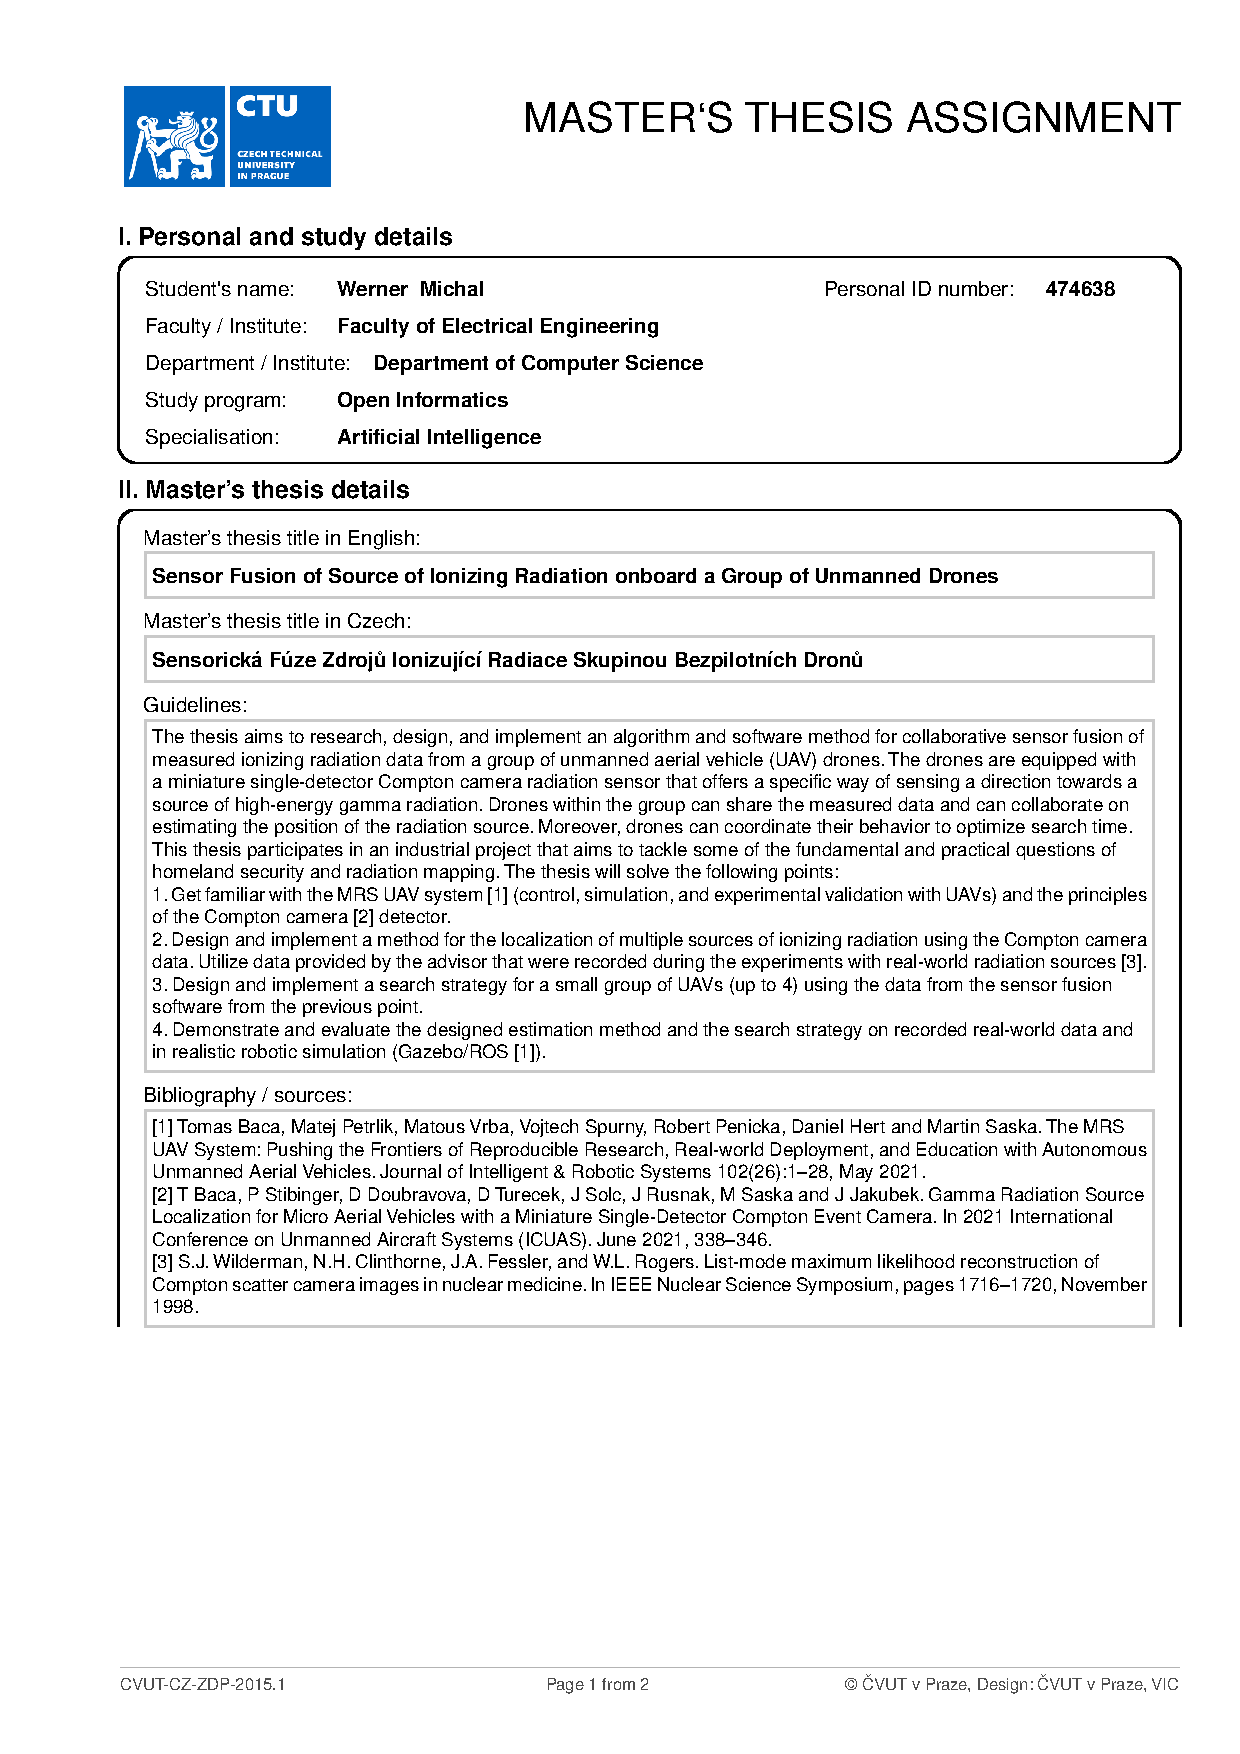
\includepdf{src/assignment.pdf}

%% --------------------------------------------------------------
%% |                          Abstracts                         |
%% --------------------------------------------------------------

\conditionalClearPage

%%!TEX root = ../main.tex

\begin{changemargin}{0.8cm}{0.8cm}

~\vfill{}

\section*{Abstract}
\vskip 0.5em

This thesis presents a method for localizing multiple sources of ionizing radiation using a group of \acp{UAV}. 
These \acp{UAV} are equipped with miniature single-detector Compton camera radiation sensors, enabling them to estimate the directions towards high-energy gamma radiation sources.
  The proposed radiation mapping method (utilizing a \ac{MLE} principle) fuses the measurements from the Compton camera sensors to accurately estimate the positions of radioactive sources during the flight.
The properties of the used detector are approximated using Monte Carlo simulation techniques.
The estimation method is combined with an active search strategy that coordinates future action of the drones in order to improve the quality of estimate of sources position and minimize search time.
%In addition, an active search strategy is incorporated into the system, coordinating the future actions of the drones. 
%This strategy aims to improve the quality of the estimated source positions and minimize the search time by efficiently exploring the designated area of interest.
The proposed solution is evaluated on recorded real world data and in realistic simulator.





  \mycomment{
%The study of autonomous \acp{UAV} has become a prominent sub-field of mobile robotics.

This thesis presents a method for localization of multiple sources of ionizing radiation using a group of autonomous \acp{UAV} 
that are equipped with a miniature single-detector Compton camera radiation sensor capable of estimating directions towards a source of high-energy gamma radiation.
The proposed radiation mapping method (based on a \ac{MLE} principle) fuses the measurements from the Compton camera sensors and estimates the positions of radioactive sources during the flight.
Properties of the detector are approximated using Monte Carlo simulation.
The estimation method is combined with an active search strategy that coordinates future action of the drones in order to improve the quality of estimate of sources position and minimize search time.
The solution is evaluated on recorded real world data and in realistic simulator.
%The proposed estimation method based on maximum likelihood principle fuses the Compton camera measurements and estimates the positions of radioactive sources during the flight.
%The MiniPIX TPX3 Compton camera is can electronvolt
%The proposed solution utilizes a data fusion method based on \ac{MLEM} algorithm, which combines measurements from multiple \acp{UAV} and estimates the positions of radioactive sources during the flight.
%The fusion method 

%  for fusing the measurements
%and estimating the radiation source position during the flight.
}
\vskip 1em

{\bf Keywords} \Keywords

\vskip 2.5cm

\end{changemargin}


\conditionalClearPage

%%!TEX root = ../main.tex

\begin{changemargin}{0.8cm}{0.8cm}

~\vfill{}

\section*{Abstrakt}
\vskip 0.5em

\sloppy
Výzkum na poli autonomních bezpilotních prostředků (UAV) se stal významným oborem mobilní robotiky.

\vskip 1em

{\bf Klíčová slova} \KlicovaSlova

\vskip 2.5cm

\end{changemargin}


%% --------------------------------------------------------------
%% |                        Abbreviations                       |
%% --------------------------------------------------------------

\conditionalClearPage

\begin{changemargin}{0.8cm}{0.8cm}

~\vfill{}

\section*{Abbreviations}

% this will print only the used abbreviations
%!TEX root = ../main.tex

\begin{acronym}
  \acro{API}[API]{Application Programming Interface}
  \acro{CTU}[CTU]{Czech Technical University}
  \acro{DOF}[DOF]{degree-of-freedom}
  \acro{FOV}[FOV]{Field of View}
  \acro{GNSS}[GNSS]{Global Navigation Satellite System}
  \acro{GPS}[GPS]{Global Positioning System}
  \acro{IMU}[IMU]{Inertial Measurement Unit}
  \acro{MLE}[MLE]{Maximum likelihood estimation}  
  \acro{LKF}[LKF]{Linear Kalman Filter}
  \acro{pix}[Minipix3]{MiniPIX TPX3}
  \acro{CS}[CS]{Compton scattering}
  \acro{PE}[PE]{Photoelectric effect}
  \acro{PET}[PET]{Positron emission tomography}
  \acro{SPECT}[SPECT]{Single Photon Emission Computed Tomography}
  \acro{FDNPP}[FDNPP]{Fukushima Daiichi Nuclear Power Plant}
  \acro{LM-MLEM}[LM-MLEM]{List-Mode Maximum Likelihood Expectation Maximization}
  \acro{MLEM}[MLEM]{Maximum Likelihood Expectation Maximization}
  \acro{MAP}[MAP]{Maximum A Posteriori}
  \acro{SOE}[SOE]{Stochastic Origin Ensemble}
  \acro{CC}[CC]{Compton camera}
  \acro{TSP}[TSP]{Travelling salesman problem}
  \acro{MAV}[MAV]{Micro Aerial Vehicle}
  \acro{MPC}[MPC]{Model Predictive Control}
  \acro{MRS}[MRS]{Multi-robot Systems Group}
  \acro{ROS}[ROS]{Robot Operating System}
  \acro{SLAM}[SLAM]{Simultaneous Localization And Mapping}
  \acro{UAV}[UAV]{Unmanned Aerial Vehicle}
  \acro{UGV}[UGV]{Unmanned Ground Vehicle}
\end{acronym}


\vskip 2.5cm

\end{changemargin}

\conditionalClearPage

%% --------------------------------------------------------------
%% |                      Table of contents                     |
%% --------------------------------------------------------------

\tableofcontents

\conditionalClearPage

% set up the full page style with normal page numbering
\pagestyle{full}
\pagenumbering{arabic}

%% --------------------------------------------------------------
%% |                        introduction                        |
%% --------------------------------------------------------------

%!TEX root = ../main.tex

\chapter{Introduction\label{chap:introduction}}

First, introduce the reader to the research topic.
Start with the most general view and slowly converge to the particular field, sub-field, and the challenges you face.
You can cite others' work here \cite{baca2021mrs}.

\section{Related works}

This section should contain related state-of-the-art works and their relation to the author's work.
We usually cite the original works like this \cite{benallegue2008high}.
You can also cite multiple papers at once like this \cite{baca2016embedded, baca2021mrs}.




\subsection{ MRS paper}
This thesis builds on the work of the MRS group (Faculty of Electrical engineering, CTU in Prague) in the field of radiation mapping. 
This paper \cite{baca2021gamma} presents a multi-robotic approach to an autonomous localisation of a compact gamma radiation source. 
All unmanned aerial vehicles are equipped with compact MiniPIX TPX3 CdTe event camera, which is capable of measuring gamma particles and reconstructing Compton events. 
The output of the sensor are Compton cones are used for localisation in the following way:
in the first phase of autonomous exploration, the \ac{UAV}s are exploring the area to measure the first Compton cones. 
After the first eight cones are reconstructed, their intersection is computed using optimisation methods (quadratic programming). 
This initial estimate is then incrementally updated using new measurements. 
The current estimate is always orthogonally projected to the newly measured cone. 
These measurements are fused using \ac{LKF}. 
The \ac{UAV}s are controlled in a way that they encircle the current estimate in order to measure more cones and update the \ac{LKF} estimate.

Using this approach, the group of drones is capable to localise a single compact source of ionising radiation. 
The source can be static or dynamic. 
However, this iterative method cannot localise multiple sources of radiation.
Once the drones detect one source of radioactive particles, they start encircling the current estimate and cannot find other sources in the area.

The main purpose of this thesis is to improve the presented solution: introduce a new method that could localise multiple sources of ionising radiation and control group of \ac{UAV}s to explore the whole area and maximise information gain given the specific sensor.



\section{TODO}
\begin{itemize}
\item clanek MRS ze ktereho vychazim
\item diplomka Petra Štibingera
\item ostatni robotické články týkající se robotickeho pruzkumu, leteckeho nebo pozemniho
\end{itemize}
\section{Contributions}

This section should describe the author's contributions to the field of research.

\section{Mathematical notation}

It is a good practice to define basic mathematical notation in the introduction.
See \reftab{tab:mathematical_notation} for an example.

\begin{table*}[!h]
  \scriptsize
  \centering
  \noindent\rule{\textwidth}{0.5pt}
  \begin{tabular}{lll}
    $\mathbf{x}$, $\bm{\alpha}$ & vector, pseudo-vector, or tuple\\
    $\mathbf{\hat{x}}$, $\bm{\hat{\omega}}$& unit vector or unit pseudo-vector\\
    $\mathbf{\hat{e}}_1, \mathbf{\hat{e}}_2, \mathbf{\hat{e}}_3$ & elements of the \emph{standard basis} \\
    $\mathbf{X}, \bm{\Omega}$ & matrix \\
    $\mathbf{I}$ & identity matrix \\
    $x = \mathbf{a}^\intercal\mathbf{b}$ & inner product of $\mathbf{a}$, $\mathbf{b}$ $\in \mathbb{R}^3$\\
    $\mathbf{x} = \mathbf{a}\times\mathbf{b}$ & cross product of $\mathbf{a}$, $\mathbf{b}$ $\in \mathbb{R}^3$\\
    $\mathbf{x} = \mathbf{a}\circ\mathbf{b}$ & element-wise product of $\mathbf{a}$, $\mathbf{b}$ $\in \mathbb{R}^3$ \\
    $\mathbf{x}_{(n)}$ = $\mathbf{x}^\intercal\mathbf{\hat{e}}_n$ & $\mathrm{n}^{\mathrm{th}}$ vector element (row), $\mathbf{x}, \mathbf{e} \in \mathbb{R}^3$\\
    $\mathbf{X}_{(a,b)}$ & matrix element, (row, column)\\
    $x_{d}$ & $x_d$ is \emph{desired}, a reference\\
    $\dot{x}, \ddot{x}, \dot{\ddot{x}}$, $\ddot{\ddot{x}}$ & ${1^{\mathrm{st}}}$, ${2^{\mathrm{nd}}}$, ${3^{\mathrm{rd}}}$, and ${4^{\mathrm{th}}}$ time derivative of $x$\\
    $x_{[n]}$ & $x$ at the sample $n$ \\
    $\mathbf{A}, \mathbf{B}, \mathbf{x}$ & LTI system matrix, input matrix and input vector\\
    \emph{SO(3)} & 3D special orthogonal group of rotations\\
    \emph{SE(3)} & \emph{SO(3)}~$\times~\mathbb{R}^3$, special Euclidean group\\
  \end{tabular}
  \noindent\rule{\textwidth}{0.5pt}
  \caption{Mathematical notation, nomenclature and notable symbols.}
  \label{tab:mathematical_notation}
\end{table*}


%!TEX root = ../main.tex

\chapter{Preliminaries\label{chap:preliminaries}}

\section{Radioactivity}
Radioactivity is a natural phenomenon in which unstable atomic nuclei undergo spontaneous decay, emitting radiation in the form of particles or electromagnetic waves. 
This process occurs in certain types of atoms, known as radioactive isotopes or radionuclides. 
The radioactive atom aims to achieve a state of stability by dispensing energy in the form of ionizing radiation.
Ionizing radiation refers to any form of radiation with enough energy to remove tightly bound electrons from the orbit of an atom.
Among others, radioactive decay releases three main types of ionizing radiation: alpha, beta and gamma. 

\section{Some properties of ionizing radiation}

\subsection{Health risks}% %%{
Several health risks are associated with ionizing radiation.
While traversing the human body, ionizing radiation can interact with living tissues causing damage or mutations of individual cells.
In the long-term horizon, exposure to ionizing radiation might cause cancer or even genetic disorders.
The severity of health problems depends on the exposure time and dose of absorbed radiation.
High doses of ionizing radiation over a short period can cause acute radiation syndrome (radiation sickness).
The disease is manifested by nausea, vomiting, fatigue or even skin burns. 
Depending on the absorbed radioactive dose, it causes several neurological or cardiovascular problems or might lead to death.% %%}

\subsection{Activity}% %%{
``Activity'' is one of the terms used to quantify and describe the properties of radioactive sources.
It is defined as the number of radioactive decays per second.
The unit of activity is called Becquerel ($\si{\becquerel}$) and belongs to SI\footnote{International System of units} units.
In other words, if a radioactive source has activity one Becquerel, it means that one unstable nucleus decays per second (on average, since the decay is a stochastic process).
It is important to note that the Becquerel only measures the rate of decay and does not take into account the type or energy of the radiation involved.% %%}
However, for the purpose of this thesis, ``activity''  is used as the number of gamma photons emitted from the source position in any direction per second.

\subsection{Inverse square law}% %%{
The inverse square law is a fundamental principle that applies to diverse physical phenomena, including radiation.
It describes how the intensity of radiation decreases with increasing distance from the source.
The intensity of radiation is inversely proportional to the square distance from the source:
\begin{equation}
  intensity \approx \frac{1}{distance^2}.
\end{equation}
For example, doubling the distance to the source means that the intensity decreases to $\frac{1}{4}$.
As illustrated in figure \ref{fig:islaw}, this principle comes from the fact that the radiation spreads out over a larger area when the observer is further away from the source.
This rapid decrease makes the search for sources of ionizing radiation challenging since it limits the sensing range of the detectors.

  \begin{figure}[!h]
    \centering
      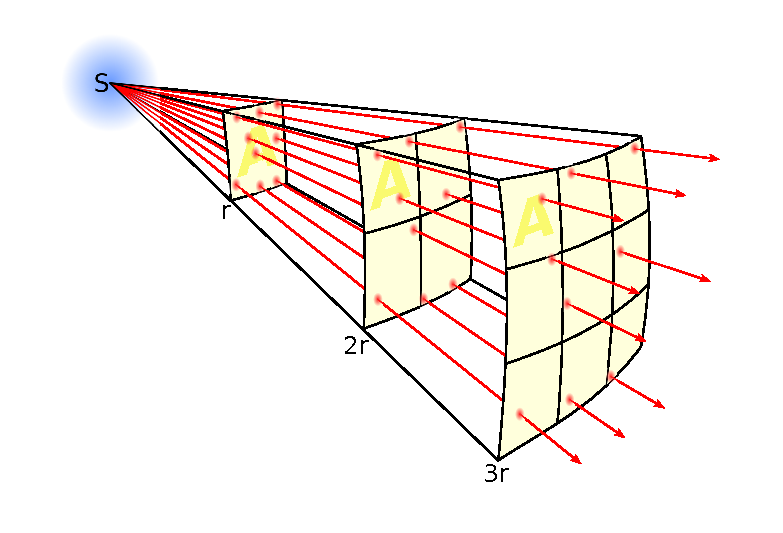
\includegraphics[width=0.65\textwidth]{./fig/photos/Inverse_square_law.eps}
    \caption{An illustration of the inverse square law for the intensity of radiation. Source: \cite{inverse_square_law}}
      \label{fig:islaw}
  \end{figure}

% %%}
\section{Main types of ionizing radiation}
\subsection{Alpha radiation}
Alpha radiation is an emission of positively charged alpha particles consisting of two protons and two neutrons bound together (helium nuclei).
This gives alpha particles a significantly larger mass and higher reactivity compared to other types of ionizing radiation.
On the other hand, they interact strongly with matter and can't penetrate far.
Alpha particles can travel only a few centimetres in the air and can be blocked by a single sheet of paper or the outer layer of human skin.
Because of that, external sources of alpha radiation are generally not considered a significant threat to human health.
The limited range of alpha radiation makes it difficult to sense from a distance.

\subsection{Beta radiation}
Beta particles are high-energy, high-speed electrons or positrons.
Due to their smaller size and weaker electrical charge, they are generally more penetrating and less reactive than alpha particles and can reach further into materials.
Several centimetres thick sheet of aluminium or plastic is typically sufficient to block the beta radiation.
In terms of travel through the air, beta particles have a range of a few meters.
Although beta radiation is generally less dangerous than gamma, when particles come into contact with human skin, they can penetrate the outer layers and cause skin burns as the particles disrupt cellular processes.

\subsection{Gamma radiation}
Gamma particles are often produced alongside alpha or beta particles during radioactive decay. 
Unlike them, gamma radiation of composed of high-energy photons. 
They are extremely penetrating and can travel long distances in the air and get through most of materials or living tissues thanks to their high energy and lack of charge.
Only a thick layer of concrete or lead might block this type of ionizing radiation.
These features make gamma radiation significantly more dangerous than alpha and beta.
The long-range of gamma radiation, together with its negative effects on human health, makes it an ideal candidate for remote sensing and detection.
  \begin{figure}[!h]
    \centering
      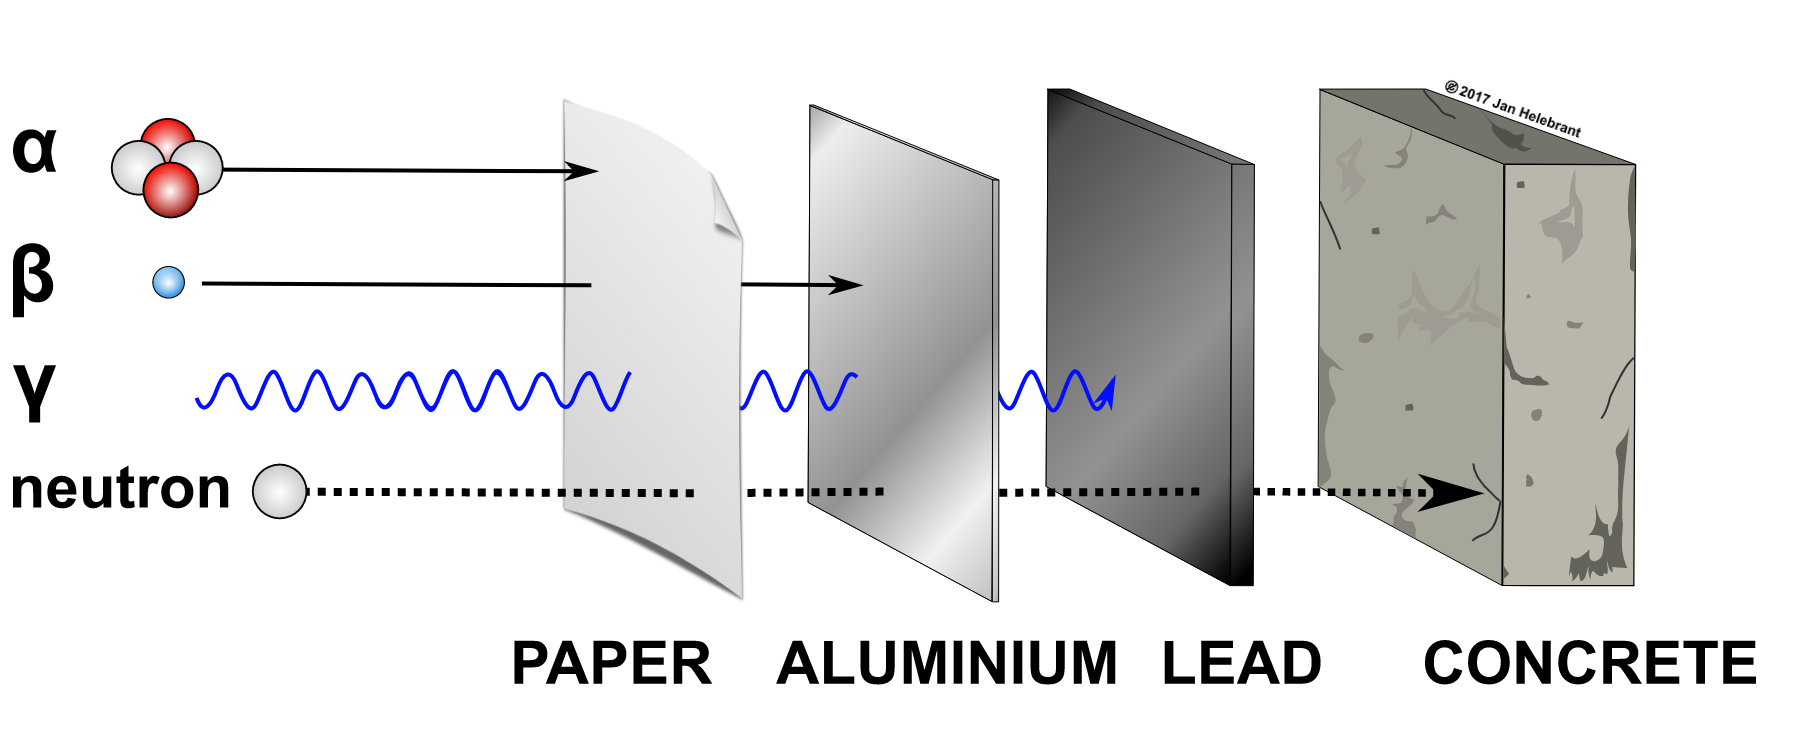
\includegraphics[width=0.6\textwidth]{./fig/photos/pene2.png}
    \caption{Penetrating power of different types of radiation. Source: \cite{penetrating_power}}
      %\label{fig:islaw}
  \end{figure}

\subsubsection{Cesium-137}
Cesium-137 is a radioactive isotope of cesium and one of the most common bi-products of nuclear fission.
It is used in radiotherapy in medicine, for calibration of radiation detection equipment in the industry and 
(most importantly) it is one of the most common fission products by the nuclear fission of uranium-235, which is used as a fuel in nuclear power plants and in nuclear weapons.
Cesium-137 is also the main source of radioactive pollution caused by accidents in Chornobyl (1986) and Fukushima (2011).
The half-life (defined as the interval of time required for one-half of the atomic nuclei of a radioactive sample to decay) of cesium-137 is $30.05$ years.
It is important to note that cesium-137 itself is not a source of $\gamma$ radiation.
However, it decays by beta emission to metastable Barium-137, which decays almost immediately (with a half-life of about $2.5$ minutes) and emits $\gamma$ photons with initial energy $\SI{662}{\kilo\electronvolt}$.
Cesium-137 (with its long half-life, negative health effects, wide usage and high penetrating power of $\SI{662}{\kilo\electronvolt}$ photons) is a good candidate for remote sensing. 
The methods proposed in this thesis have been tested using Cesium-137 radioactive isotope as a source of radiation (during simulated and real-world experiments).

\section{Interaction of $\gamma$ radiation with matter}
Sensing of $\gamma$ radiation is possible through interactions of ionizing photons with imaging devices.
%A variety of interactions may take place as a high-energy photon travels through matter.
Several interactions might occur when a high energetic photon travels through matter.
Type of the interaction depends on both the energy of the incoming photon and the properties of the material it encounters. 
%epending on the energy of the incoming photon as well as on the properties of material.
%Three main types of interactions are: a photoelectric effect, Compton scattering and pair production.
The three primary types of interactions include the photoelectric effect, Compton scattering, and photon-electron pair production.
Figure \ref{fig:dominant} describes the dominant type of interactions depending on the energy of the incoming photon and the atomic number of the material.

\subsection{Photoelectric effect and pair production}
In \ac{PE}, alternatively referred to as photoelectric absorption, the $\gamma$ photon interacts with an orbital electron of the absorbing atom.
The photon transfers all its energy to the electron and disappears.
As a consequence, the electron exceeds its binning energy and is emitted from the atom.
Photoelectric absorption is dominant at lower energies of the incident photon, although it can occur at any photon energy.
The \ac{PP} occurs only if the $\gamma$ photon has energy exceeding $\approx \SI{1}{\mega\electronvolt}$.
In this case, the highly energetic photon interacts with the atom's nucleus. 
The interaction results in the creation of an electron-positron pair.

\begin{figure}[!h]
  \centering 

    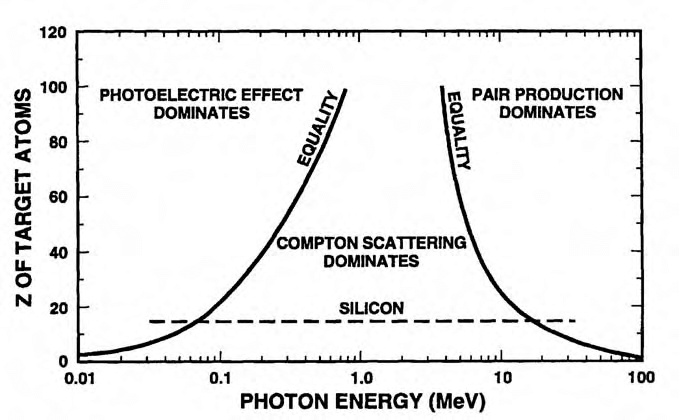
\includegraphics[width=0.6\textwidth]{./fig/photos/dominant.png}
  \caption{Dominant types of interactions for different energy of photon (x-axis) and atomic number of material (y-axis). Source of image: \cite{schwank}}
    \label{fig:dominant}
  
\end{figure}

\subsection{Compton scattering}
The third potential interaction, primarily prevalent at mid-level energies, is Compton scattering.
In this process, the $\gamma$ photon interacts with an electron that is loosely attached to the nucleus. 
The photon, with its initial energy $E_{0}$, transfers a portion of its energy to the electron.
As a result of the interaction, the lower energetic photon with energy $E_{2}$ is scattered and emitted in a direction changed by angle $\beta$. 
The energy difference $E_{1} = E_{0} - E_{2}$ is transferred to a bi-product of the interaction --- an electron.
The situation is illustrated in figure \ref{fig:scattering}.
According to Compton \cite{compton}, the relation of particle energies and scattering angle $\beta$ can be expressed as:
\begin{equation}
E_{2} = \frac{E_{0}}{  1 + (E_{0} / m_{e}c^{2}) (1 - \mathrm{cos} \beta)},
  \label{eq:compton_energies}
\end{equation}
where $E_{0}$ is the initial energy of the incoming photon, $E_{2}$ is the energy of scattered photon,  $m_{e}$ is the electron rest mass and $c$ is the speed of light in vacuum. 
\begin{figure}[!h]
    \centering
    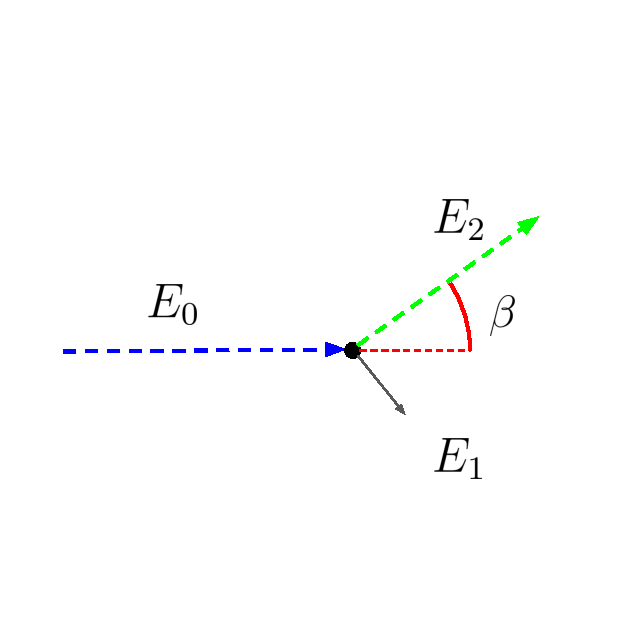
\includegraphics[width=0.4\textwidth]{./fig/photos/compton_simple2.eps}
    \caption{An illustration of the Compton scattering. The incident $\gamma$ photon with energy $E_{0}$ (blue) undergoes the Compton scattering. As a result of the interaction, the lower energetic photon (green) with energy $E_{2}$ is emitted under angle $\beta$. Part of the energy ($E_{1}$) is transferred to a bi-product of the interaction- the electron (grey).}
    \label{fig:scattering}
\end{figure}

\mycomment{ %klein nishina % %%{
  The probability that a photon with an energy $E_{0}$ undergoes a Compton scattering through an angle $\beta$ is described by the Klein-Nishina formula
  \begin{equation}
    K(\beta, E_{0}) = \frac{r_{e}^{2}}{2} \left( \frac{E_{2}}{E_{0}}  \right)^{2} \left(  \frac{E_{2}}{E_{0}} + \frac{E_{0}}{E_{2}} - \mathrm{sin}^{2}(\beta)  \right),
    \label{eq:klein_nishina}
  \end{equation}
  where $r_{e}$ is the classical electron radius. 
}% %%}

\mycomment{% %%{
  \section{Measuring radioactivity}
  Ionizing radiation is unperceivable by human senses yet poses a significant health risk for human beings.
  Effective monitoring methods are therefore needed to detect and measure the presence of such radiation. %, that is potentially harmful to human beings.
  %Sensors of ionizing radiation are made of different materials that interact with ionizing particles.
  Therefore, efficient methods for monitoring and detecting this type of radiation are essential. 
  Various materials that interact with ionizing particles are used to construct sensors for ionizing radiation.

  Three common types of these sensors include Geiger-Müller counters, scintillation detectors, and semiconductor detectors (among many others).
   Geiger-Müller counters are tubes filled with gas that, when ionized by passing particles, conduct an electrical charge proportional to the detected particle flux.
  Scintillation detectors work differently. 
  They contain a material that emits light when hit by ionizing radiation, 
  which is then transformed into an electrical signal by a photodiode. 
  The third type of detector is made from semiconductive materials sensitive to ionizing photons. 
  The ejected electrons from the ionization process can be measured to deduce the type and energy of the incoming radiation.

  Most of these sensors function by counting the number of particles detected, thus estimating the intensity of the particle flux at the sensor's location. 
  However, this does not provide information about the direction from which the particles are coming. 
  Following \cite{baca2019timepix}, the direction of incoming particles can be deduced by different detector configurations illustrated in figure \ref{fig:sensor_overview}.
  \textbf{Pinhole camera aperture} (which is based on same principles as pinhole camera in classical optics) consists of a small hole in shielding material (e.g. lead), blocking all rays in other directions.
  This approach significantly reduces the field of view of the camera. 
  \textbf{Colimators} (frequently used in medical imaging) also restrict the set of possible directions.
  The openings in the shielding material are organized in a way that each part of the detector is responsible for measuring particles coming from certain direction.
  \textbf{Stacked detectors} employ multiple layers of detectors, where the particle's direction is computed from multiple interactions as the ray passes through the layers.
  Finally, the \textbf{Compton camera} use the Compton scattering for deducing the set of possible directions of the original particle. 



  %Each of the proposed methods have some drawbacks in context of deployment onboard a small \ac{UAV}.
  Intensity-only detectors must be relative large to get accurate measurements (collect enough interactions and compensate the stochastic nature of radioactive decay).  
  Moreover, localization of multiple sources might require many measurements at different positions, which is time consuming.
  The use of collimators or pin-hole apertures is not possible due to their limited field of view and large weight and dimensions (caused by the presence of shielding material, which must be thick enough to effectively block the other rays).
  Multi-stack detectors are complicated 
  \begin{figure}[!h]
      \centering
      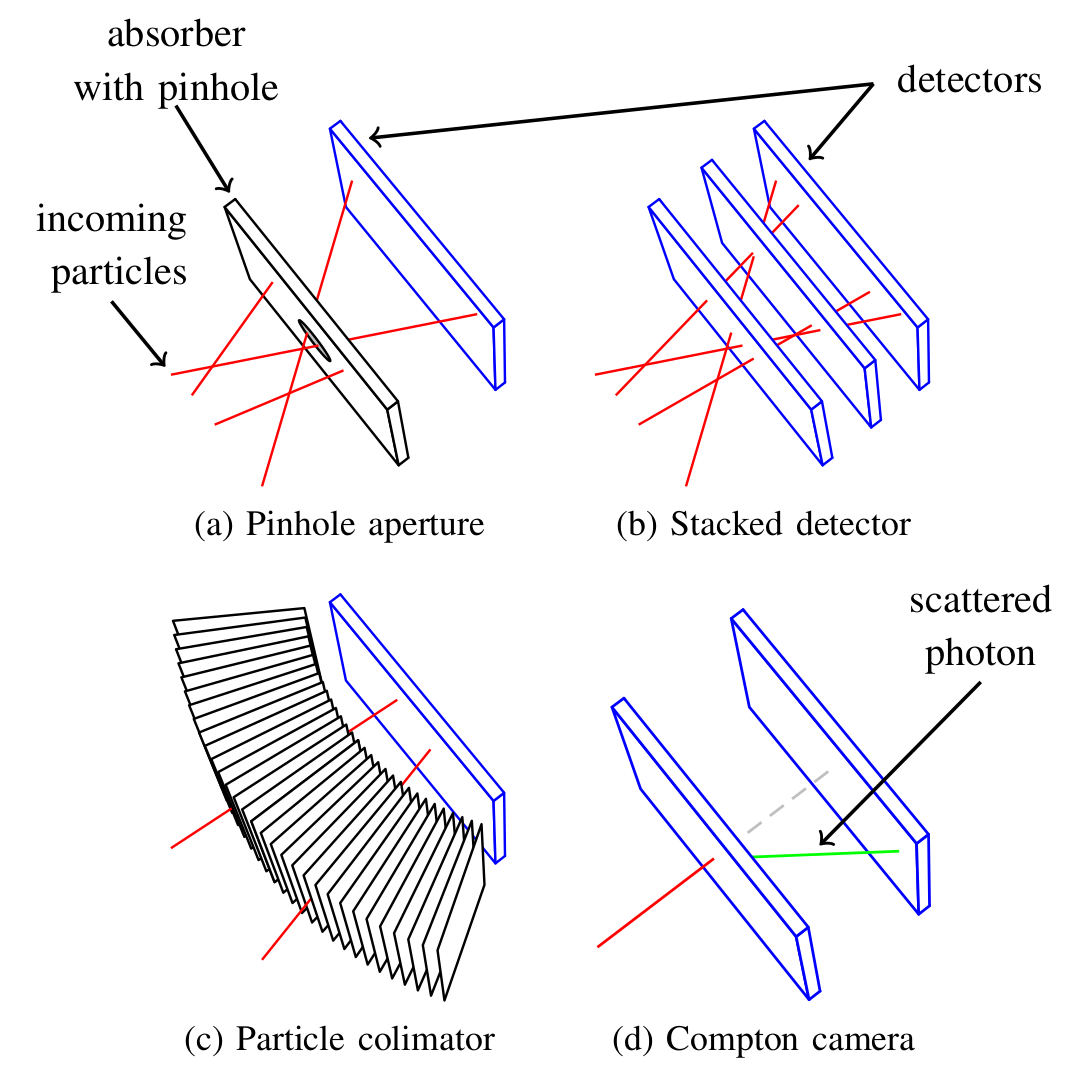
\includegraphics[width=0.5\textwidth]{./fig/photos/detector_overview_baca2019.png}
      \caption{Different ways how to deduce the direction of the incoming particle. Source: \cite{baca2019timepix}}
      \label{fig:sensor_overview}
  \end{figure}
}% %%}

\mycomment{% %%{
\begin{figure}[!h]% %%{
  \centering
  \subfloat[\centering different ways how to detect the direction of incoming particle. Source: \cite{baca2019timepix}] {
    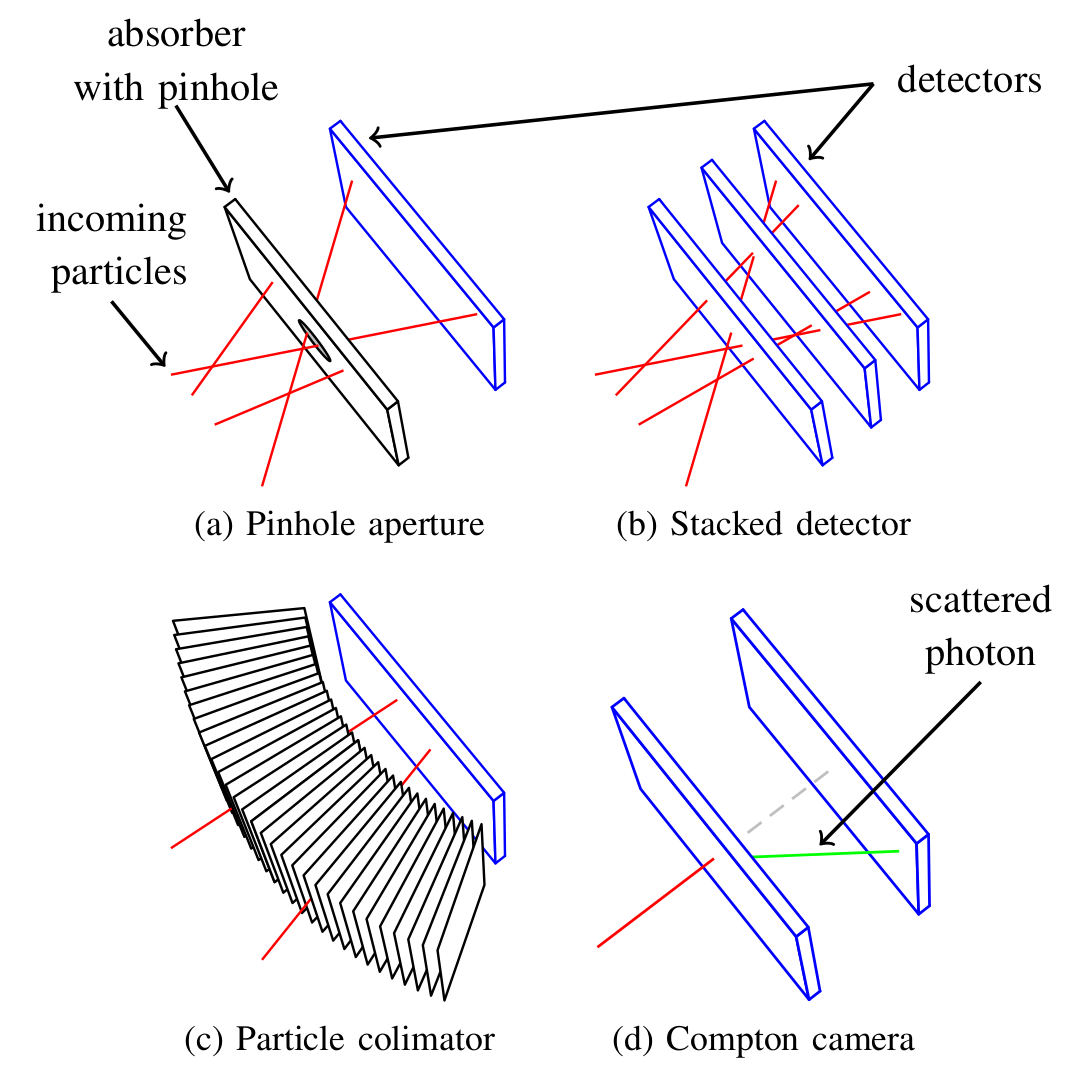
\includegraphics[width=0.49\textwidth]{./fig/photos/detector_overview_baca2019.png}
    \label{fig:sensor_overview}
  }
  \subfloat[\centering Geometry for two-layer Compton camera. The $\gamma$ particle emitted at position $j$ interacts with the first layer of the sensor (scatterer) at position $X_{1}$. A lower energetic photon is scattered under angle $\beta$ and absorbed by the second layer of the detector (absorber) at position $X_{2}$. The reconstructed Compton cone is parametrized by angle $\beta$, axis vector $a$ and origin of the cone $X_{1}$.] {
      \label{fig:compton_camera_geometry}
  
      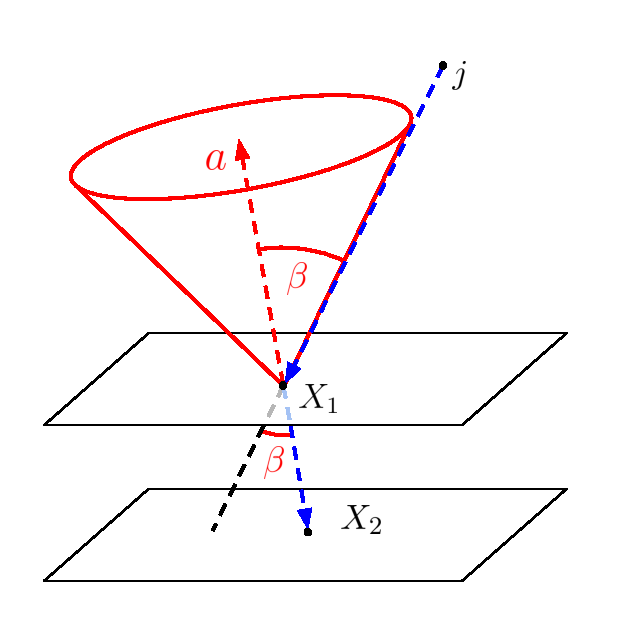
\includegraphics[width=0.49\textwidth]{./fig/photos/compton_camera_modelll.eps}
  }
  \caption{TODO}
  \label{fig:xxx}
\end{figure}% %%}
}% %%}

%%%%%%%%%%%%%%%%%%%%%%%%%%%%%%%%%%%%%%%
\section{Measuring the gamma radiation}
Ionizing radiation is unperceivable by human senses yet poses a significant health risk for human beings. 
Therefore, efficient methods for monitoring and detecting this type of radiation are essential. 
%Various materials that interact with ionizing particles are used to construct sensors for ionizing radiation.
The primary operating mode of most sensors of radioactivity is counting the number of particles detected,
thus estimating the intensity of the particle flux at the sensor's location. 
However, the dosimetric measurements do not provide information about the direction from which the radiation is emitted. 
Intensity-only detectors must be relatively large to get accurate measurements (must collect enough interactions and compensate for the stochastic nature of radioactive decay).
Moreover, the localization of multiple sources might require many measurements at different positions, which is time-consuming. 
The direction of incoming $\gamma$ photons might be deduced using
the Compton camera, which is based on the Compton scattering principle.

\mycomment{% %%{
Ionizing radiation is unperceivable by human senses yet poses a significant health risk for human beings.
%Sensors of ionizing radiation are made of different materials that interact with ionizing particles.
Therefore, efficient methods for monitoring and detecting this type of radiation are essential. 
Various materials that interact with ionizing particles are used to construct sensors for ionizing radiation.

The basic operation mode of these sensors is counting the number of particles detected, thus estimating the intensity of the particle flux at the sensor's location.
The dosimetric measurements do not provide information about the direction from which direction the radiation is emitted. 
Intensity-only detectors must be relative large to get accurate measurements (must collect enough interactions and compensate the stochastic nature of radioactive decay).  
Moreover, localization of multiple sources might require many measurements at different positions, which is time consuming.
The direction of incoming $\gamma$ photons might be deduced using the Compton camera, which is based on the Compton scattering principle.
}% %%}
\mycomment{% %%{
  %The 
  Geiger-Müller counters, scintillation detectors, and semiconductor detectors (among many others).
   Geiger-Müller counter a tube filled with gas that, when ionized by passing particles, conducts an electrical charge corresponding to the detected particle flux.
  Scintillation contains a luminescent material that emits light when hit by ionizing radiation, 
  which is then transformed into an electrical signal by a photodiode. 
  The third common type of detector is made from semiconductive materials sensitive to ionizing radiation. 
  The ejected electrons from the ionization process can be measured to deduce the type and energy of the incoming radiation.
}% %%}
\subsection{Compton Camera}% %%{
The Compton camera is typically composed of two detectors: a scatterer and an absorber.
The incident photon with energy $E_{0}$ first interacts with the scatterer at position $X_{1}$ in the form of Compton scattering.
A bi-product of the interaction (electron with energy $E_{1}$) is immediately captured by the scatterer, and its position $X_{1}$ and energy are recorded.
As a result of the interaction, a lower energetic photon with energy $E_{2}$ is scattered under (Compton) angle $\beta$.
The scattered photon then interacts in the form of \ac{PE} with the absorber.
The absorbed energy $E_{2}$ and the position of the interaction $X_{2}$ are measured and recorded.

The scattering angle $\beta$ can be reconstructed (following \cite{baca2021gamma}) from equation \ref{eq:compton_energies} as:
\begin{equation}
  %\beta = \mathrm{arccos} \left (  1-\frac{m_{e}c^{2}E_{2}}{E_{0} (E_{0} - E_{2})} \right )
  \beta = \mathrm{cos}^{-1} 
  \underset{B}{\underbrace{\left (
   1+m_{e}c^{2} \left( \frac{1}{E_{1}+E_{0}} - \frac{1}{E_{0}}\right )  \right )
  }},
    \label{eq:compton_beta_formula}
\end{equation}
assuming that $0<B<1$.
Since Compton scattering is a symmetrical phenomenon,  the set of possible directions of incoming particles forms a surface of a cone.
Such conical surface (denoted as Compton cone) is parametrized by the cone axis $\mathbf{a}$ (which is a straight line connecting the positions of intersections $X_{1}$ and $X_{2}$), Compton scattering angle $\beta$ and origin of the cone $X_{1}$.
The geometry is illustrated in figure \ref{fig:compton_camera_geometry}.

\begin{figure}[!h]
  \centering
    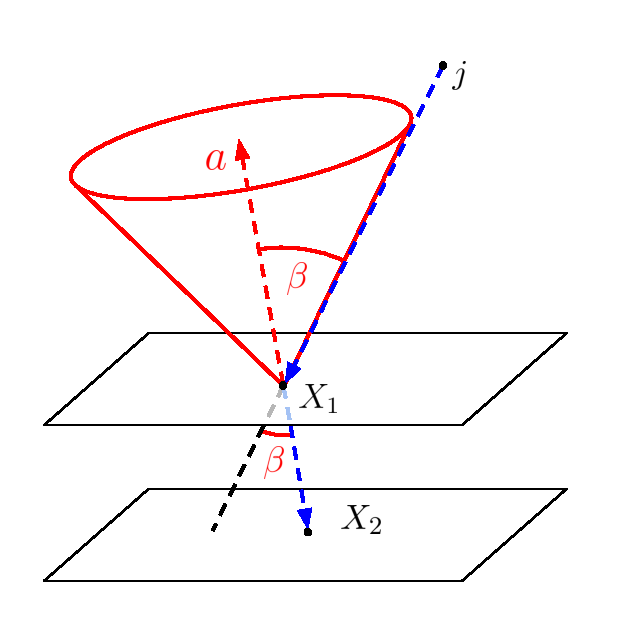
\includegraphics[width=0.4\textwidth]{./fig/photos/compton_camera_modelll.eps}
    \caption{Geometry for two-layer Compton camera. The $\gamma$ particle (emitted at position $j$) interacts with the first layer of the sensor (the scatterer) at position $X_{1}$. A lower energetic photon is scattered under angle $\beta$ and absorbed by the second layer of the detector (absorber) at position $X_{2}$. The reconstructed Compton cone is parametrized by angle $\beta$, axis vector $a$ and origin of the cone $X_{1}$.}
    \label{fig:compton_camera_geometry}
\end{figure}
% %%}
\subsection{The MiniPIX TPX3 sensor} % %%{
The MiniPIX TPX3 detector\footnote{produced by \textit{Advacam}, https://advacam.com/camera/minipix-tpx3} (in the rest of this thesis denoted as \ac{pix}) belongs to the class of semiconductor-based radiation sensors.
The \ac{pix} is composed of a) miniature version Timepix3 pixel detector \cite{timepix3},
b) the body of the sensor made of a compact block of Cadmium telluride (CdTe) semiconductor material (with dimensions $14 \times 14 \times 2 \ \si{\milli\meter}$) 
and c) necessary electronics.
The whole \ac{pix} device is very compact and lightweight (the size of the whole \ac{pix} sensor is only $80 \times 21 \times 14 \ \si{\milli\meter}$ and it weights $\SI{44}{\gram}$), therefore it can be carried onboard a small \ac{UAV}.
Unlike other devices, the \ac{pix} sensor can report the recorded $\gamma$ particles almost in real-time, which allows us to use it for an active strategy, where autonomous \ac{UAV}s react according to the measurements acquired during the flight.

Although \ac{pix} has only one detection layer, it can still be used as a Compton camera.
As described in \cite{baca2021gamma} and \cite{baca2019timepix}, the incoming ionizing radiation interacts with the matter of the sensor and separates electrons from the CdTe material.
The separated electrons are accelerated by a $\SI{450}{\volt}$ electric potential towards one facet of the sensor, where the Timepix3 pixel detector is located.
The resolution of pixel detector is $256 \times 256\ \mathrm{px}$, each pixel being $55\ \si{\micro\meter}$ large.
The pixel detector can estimate the energy of the absorbed particle and record the time when it was taken with high resolution.
Given the measured times of arrival, the coinciding products of Compton scattering might be paired together (assuming that both Compton scattering as well as follow-up photon absorption happened at the same time).

Figure \ref{fig:minipix} depicts the geometry of the \ac{pix} sensor and the detection process.
The x-axis and y-axis coordinates (see figure \ref{fig:minipix}) of the interaction are determined by the position of corresponding pixels.
The z-axis coordinate (the depth of interaction in the CdTe block) is unknown.
However, the relative z-axis distance of the two coinciding events might be deduced from the times of arrival of the two interactions captured by the pixel detector (given the known speed of electrons in the CdTe material).
The absolute z-axis coordinate is not needed since the size of the CdTe block is negligible in the context of the detection task.
More technical details related to the sensor operation are provided in \cite{baca2019timepix}.
%The \ac{pix} detector is very compact and lightweight (the size of the whole \ac{pix} sensor is only $80 \times 21 \times 14 \ \si{\milli\meter}$ and it weights $\SI{44}{\gram}$), therefore it can be carried onboard a small \ac{UAV}.
%The \ac{pix} detector can report the recorded intersections almost in real time, which allows us to use it for an active strategy, where autonomous \ac{UAV}s react according to the measurements acquired during the flight.

\begin{figure}[!h]
    \centering
  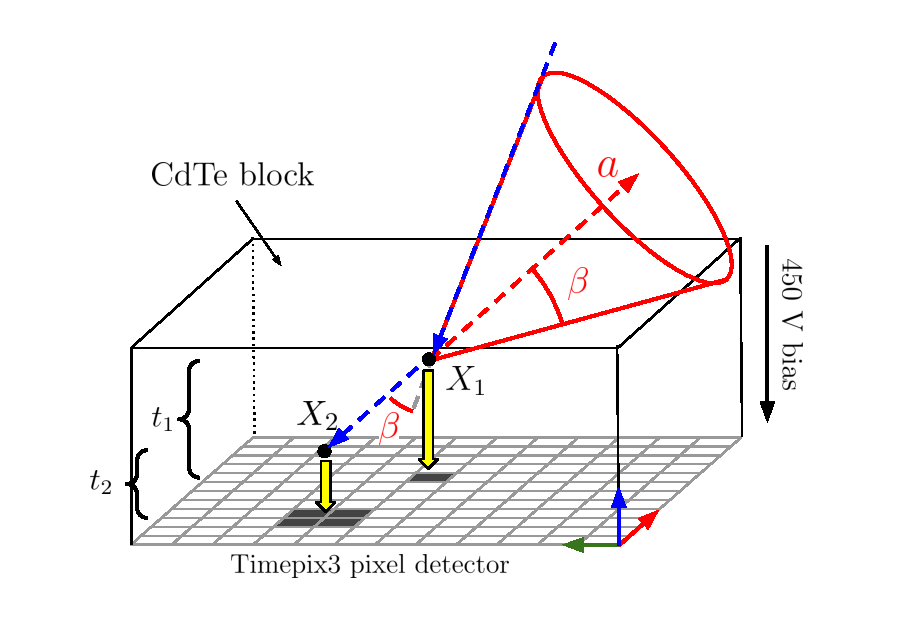
\includegraphics[width=0.7\textwidth]{./fig/photos/my_minipix.eps}
    \caption{An illustration of the detection process inside the \ac{pix} sensor. 
    The incident photon (blue) scatters under angle $\beta$ at position $X_{1}$. 
    The bi-product of the interaction (electron) is immediately absorbed. 
    Scattered photon undergoes photoelectric absorption at position $X_{2}$. 
    The free electrons (produced by the electron's absorption and scattered photon's absorption) are detected by the Timepix3 pixel detector. 2D positions ($\hat{c}_{x}, \hat{c}_{y}$) and energies ($E_{1}, E_{2}$) are recorded. 
    The relative z-axis distance between $X_{1}$ and $X_{2}$ is deduced from the time difference $t_{2}-t_{1}$ and the known speed of electrons in the CdTe block.
    The Compton cone (red) is then reconstructed.}
    \label{fig:minipix}
\end{figure}

\begin{figure}[!h]% %%{
  \centering
  \subfloat[\centering The real size of \ac{pix} sensor. Source: \cite{baca2021gamma} ] {
    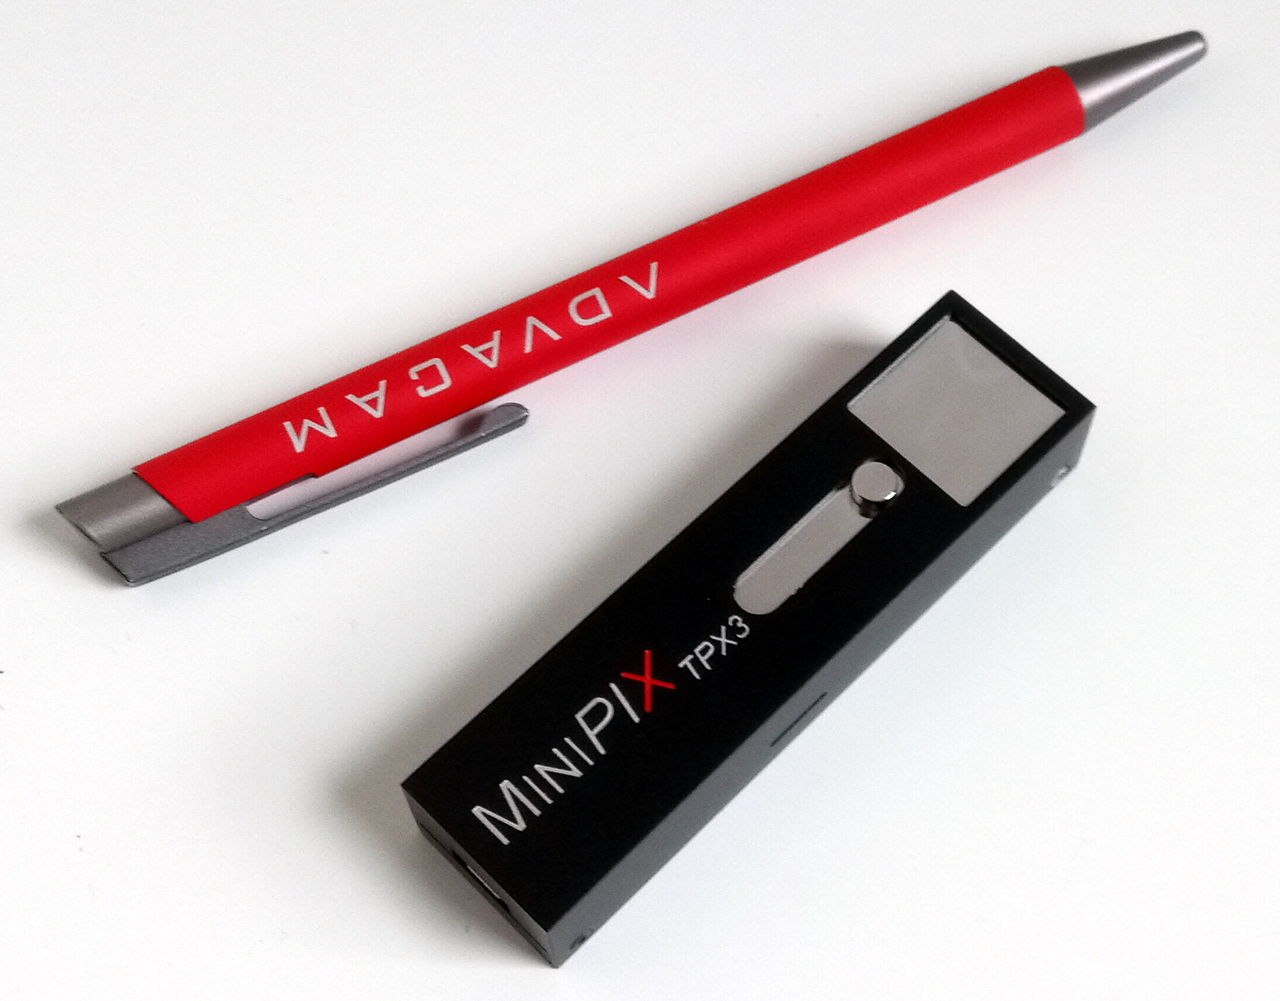
\includegraphics[width=0.35\textwidth]{./fig/photos/minipix_pen.jpg}
    \label{fig:minipix_pen}
  }
  \subfloat[\centering Pixel output of the Timepix3 detector with recorded pair of coinciding events and computed parameters of the Compton cone. Source: \cite{baca2021gamma}] {

    \begin{tikzpicture}
      \node[anchor=south west,inner sep=0] (a) at (0,0) {
          \begin{tabular}{cc}
              \fbox{
\includegraphics[width=0.25\textwidth]{./fig/rviz/timepix_10s.png}}
            &
              \fbox{
\includegraphics[width=0.25\textwidth]{./fig/rviz/timepix_10s_compton_zoom.png}}
          \end{tabular}
        };

      %%{ labels

      \begin{scope}[x={(a.south east)},y={(a.north west)}]

        \draw (0.37, 0.11) rectangle (0.43, 0.20);
        \draw[black] (0.43, 0.11) -- (0.525, 0.005);
        \draw[black] (0.43, 0.20) -- (0.525, 0.995);

        \draw (0.66,0.80) node [text=black] {\small photon track};
        \draw (0.83,0.95) node [text=black] {\small electron track};

        \draw (0.75,0.36) node [text=black] {
          \begin{tabular}{rl}
            \small $E_{1}$ = &\SI{394.22}{\kilo\electronvolt}\\
            \small $E_{2}$ = &\SI{315.70}{\kilo\electronvolt}\\
            \small $t_{2} - t_{1}$ = &\SI{20.31}{\nano\second}\\
            \small $\Delta z$ = &\SI{0.47}{\milli\meter}\\
            \hline
            \small $\beta$ = &\SI{1.13}{\radian}\\
          \end{tabular}
        };

      \end{scope}

      %%}
    \end{tikzpicture}
  %\caption{An example of a pair of Compton scattering products captured by the Timepix3 detector. The event's times are used together with the particle's energies to reconstruct the scattering angle, $\Theta$.
  \label{fig:timepix_image}





  }
  \label{fig:minipix_ilu}
  \caption{The \ac{pix} sensor and it's real size (\ref{fig:minipix_pen}) and the illustration of output from Timepix3 pixel detector (\ref{fig:timepix_image}).} 

\end{figure}% %%}

\mycomment{% %%{
\begin{figure}[!h]
    \centering
  \includegraphics[width=0.2\textwidth]{./fig/photos/minipix_in_hand.png}
    \caption{MiniPIX TPX3 sensor. Source: \url{http://mrs.felk.cvut.cz/rospix3}}
    %\label{fig:minipix}
\end{figure}
}% %%}

\mycomment{% %%{
\begin{figure}[!h]
    \centering
    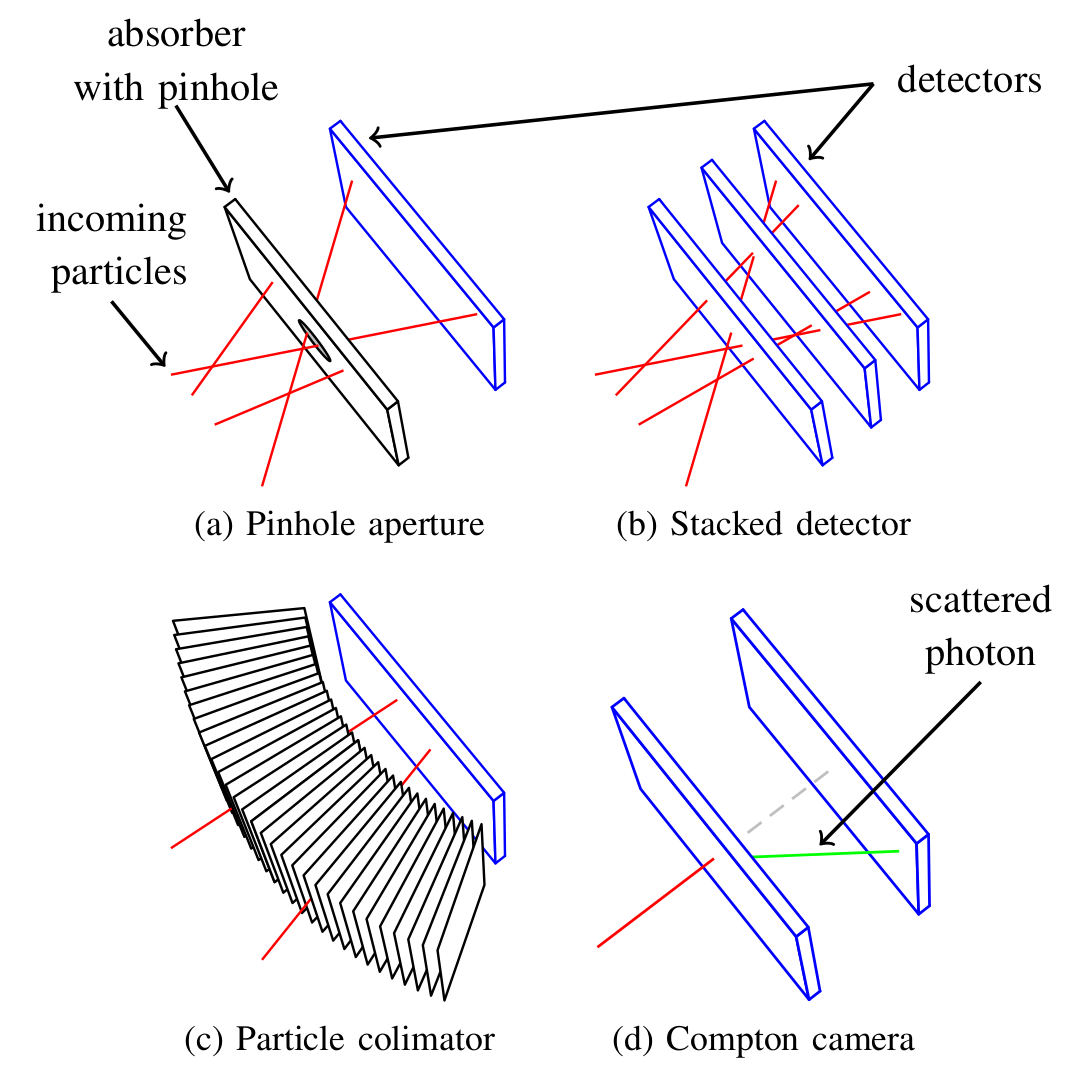
\includegraphics[width=0.5\textwidth]{./fig/photos/detector_overview_baca2019.png}
    \caption{different ways how to detect the direction of incoming particle. Source: \cite{baca2019timepix}}
    \label{fig:sensor_overview}
\end{figure}
}% %%}
% %%}

\section{Robot operating system}
The \ac{ROS} \cite{ROS} is a middleware open-source software framework for robotics applications and research.
\ac{ROS} supports for multiple programming languages, most notably \textit{Python} and \textit{C++}.
Individual software modules (called \textit{nodes}) can exchange data through a standardized communication model.
The registration of the individual \textit{nodes}, as well as communication between them, is maintained by a central authority called \ac{ROS} \textit{master}.
The main advantage of \ac{ROS} is its flexibility - multiple \textit{nodes} might be executed independently without restarting the whole program.
\ac{ROS} provides a variety of other useful tools.
\textit{TF library} keeps track of multiple coordinate frames over time and provides transformations between them.
\textit{Rosbag} is a tool for recording and playing back data collected during the experiments.
\textit{RViz} is helpful 3D graphical interface for visualisation and debugging.
%The key feature of \ac{ROS} is the \textit{transformation} library, which provides transformations between different coordinate frames of the robotic system.
%The \ac{ROS} master provides the registration of the individual \ac{ROS} nodes as well as maintains communication between them.

\subsubsection{ROS communication model}
The fundamental \ac{ROS} communication mechanism used for exchanging messages between different \ac{ROS} \textit{nodes} is called \textit{topics}.
\textit{Topics} are based on a publish-subscribe model, where nodes can either publish data to a topic or subscribe to receive data from a topic. 
Each topic has a specific data type associated with it.
Nodes can publish messages of that data type to the topic, and any subscribed nodes will receive those messages.
Topics enable asynchronous communication between different parts of the robotic system, such as data exchange between sensors and onboard computer.

Another important \ac{ROS} communication concept is called \textit{service}.
\ac{ROS} \textit{services} allow \textit{nodes} to make requests and receive responses to them.
Unlike in \ac{ROS} \textit{topics}, services provide a synchronous request-response communication model.
The client node sends its request to a specific service provided by the server node.
The server node processes the request and generates a response message, which is sent back to the sender.
Such a communication scheme might be used, for example, for triggering some action, requesting a path from the planning node and generally in any situation where a response from the server node is required.

\begin{figure}[!h]
    \centering
  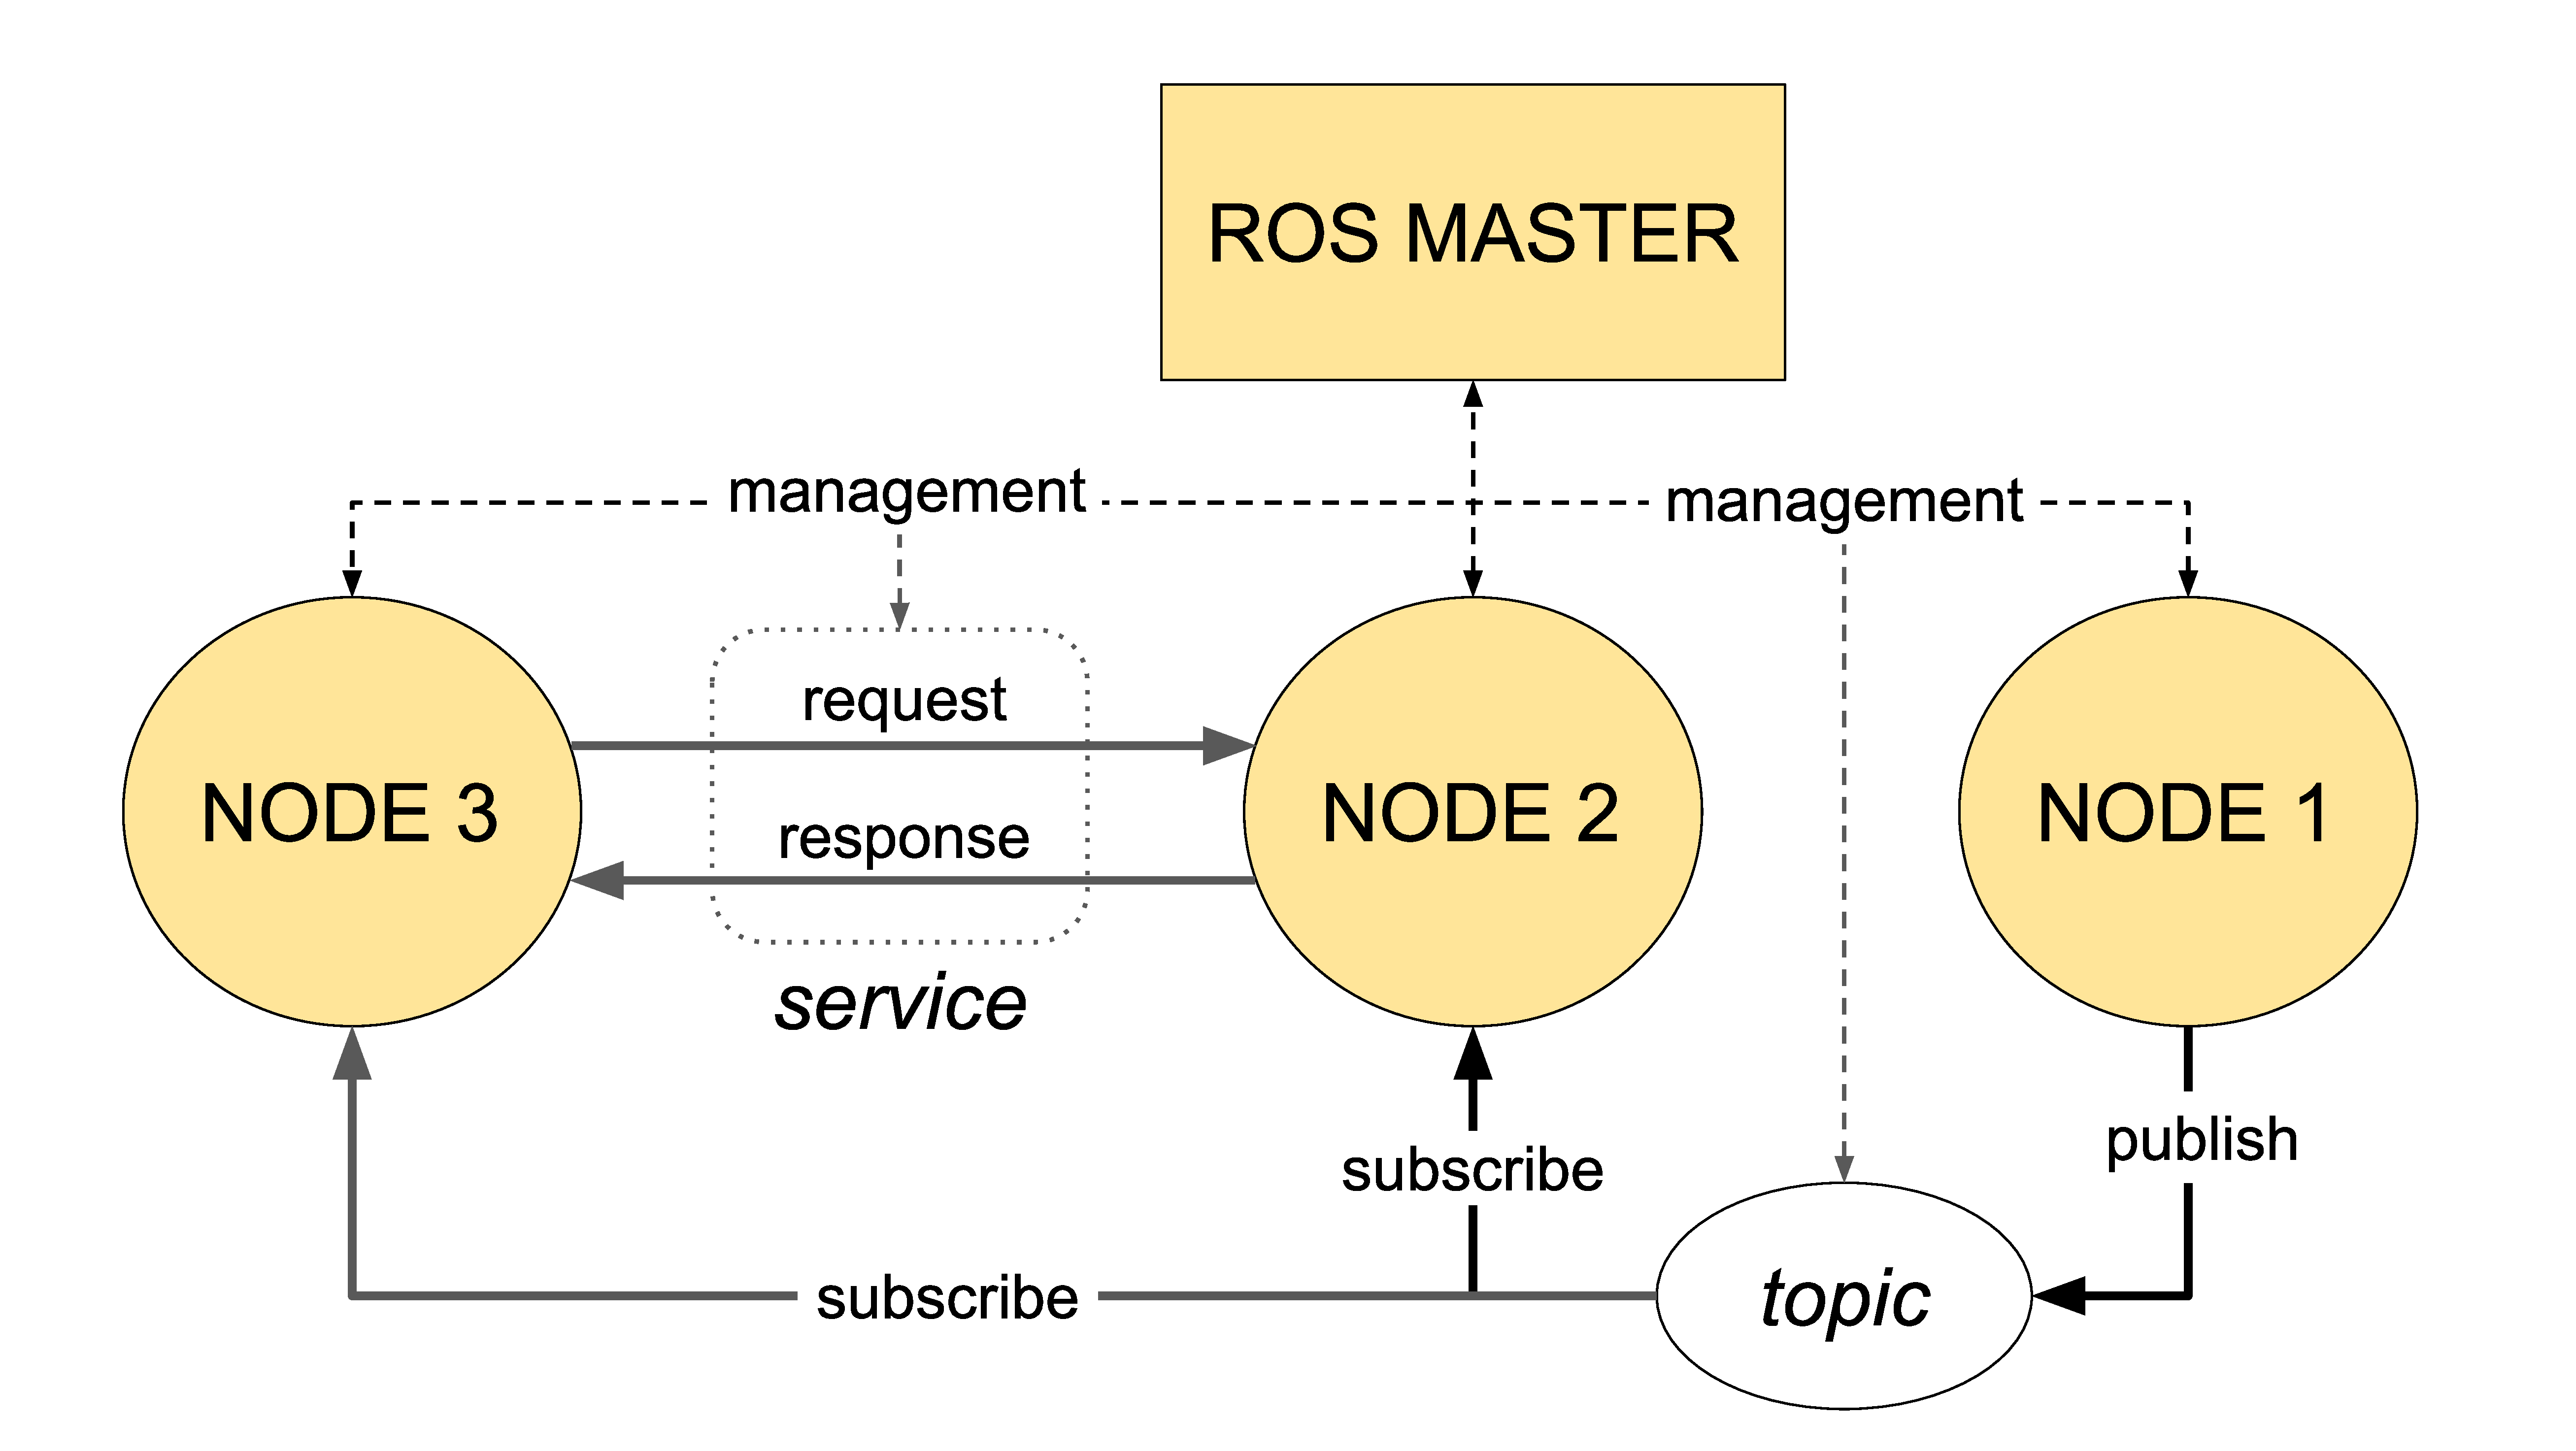
\includegraphics[width=0.8\textwidth]{./fig/photos/ros_schema.eps}
    \caption{Structure of \ac{ROS} communication model. Individual \textit{nodes} share data using \textit{topics} (publisher-subscriber model) or \text{services} (request-response model). The whole communication as well as \textit{node} registration in managed by \textit{master}.}%\url{https://www.clearpathrobotics.com/assets/guides/melodic/ros/Intro%20to%20the%20Robot%20Operating%20System.html}}
    %\label{fig:minipix}
\end{figure}

\subsection{simulations}
The simulations within this project were made using \textbf{Gazebo}, an open-source 3D simulator for robotic research.
It is fully compatible with \ac{ROS} and allows realistic simulations of robotic systems.
The ionizing radiation was simulated using \textbf{Rospix}\footnote{available at: \url{https://github.com/rospix}} simulation package.
The simulation process incorporates properties of the environment (air attenuation) as well as the geometry of the sensor and all the underlying principles leading to the detection of an ionizing photon by the Compton camera.
The properties of the simulator of ionizing radiation are described in \cite{baca2019timepix}.

\section{MRS UAV system}
The proposed high-level control method builds on the MRS UAV system\footnote{available at: \url{https://github.com/ctu-mrs/mrs_uav_system}} \cite{mrs_system}.
The MRS UAV system is a research-oriented software platform developed at Czech Technical University in Prague.
The MRS system is based on \ac{ROS} and provides full control pipeline for different types of \ac{UAV}s, including state estimation, sensor fusion, trajectory generation, multi-robot communication, planning and feedback control.
Methods proposed in this thesis builds on some parts of the MRS UAV System --- localization and state estimation (it is assumed the drones are localized using \ac{GPS} or other localization method), communication (the drones can exchange information between each other) and control (the \ac{UAV}s can execute given path).


%%%%%%%%%%%%%%%%%%%%%%%%
%%%%%%%%%%%%%%%%%%%%%%%%%%
%%%%%%%%%%%%%%%%%%%%%%%
%%%%%%%%%%%%%%%%%%%%%%%%%%%%
%%%%%%%%%%%%%%%%%%%%%%%%%%
%%%%%%%%%%%%%%%%%%%%%%%%
%%%%%%%%%%%%%%%%%%%%%%%%%%
%%%%%%%%%%%%%%%%%%%%%%%
%%%%%%%%%%%%%%%%%%%%%%%%%%%%
%%%%%%%%%%%%%%%%%%%%%%%%%%

% %%{
\mycomment{



\begin{figure}[!h]% %%{
  \centering
  \subfloat[\centering Cross-section for photon interactions in Silicon in the MeV range. The four dominating interaction mechanisms are photo effect, Compton scattering, pair creation and Rayleigh scattering. Source: \cite{zoglauer}] {
    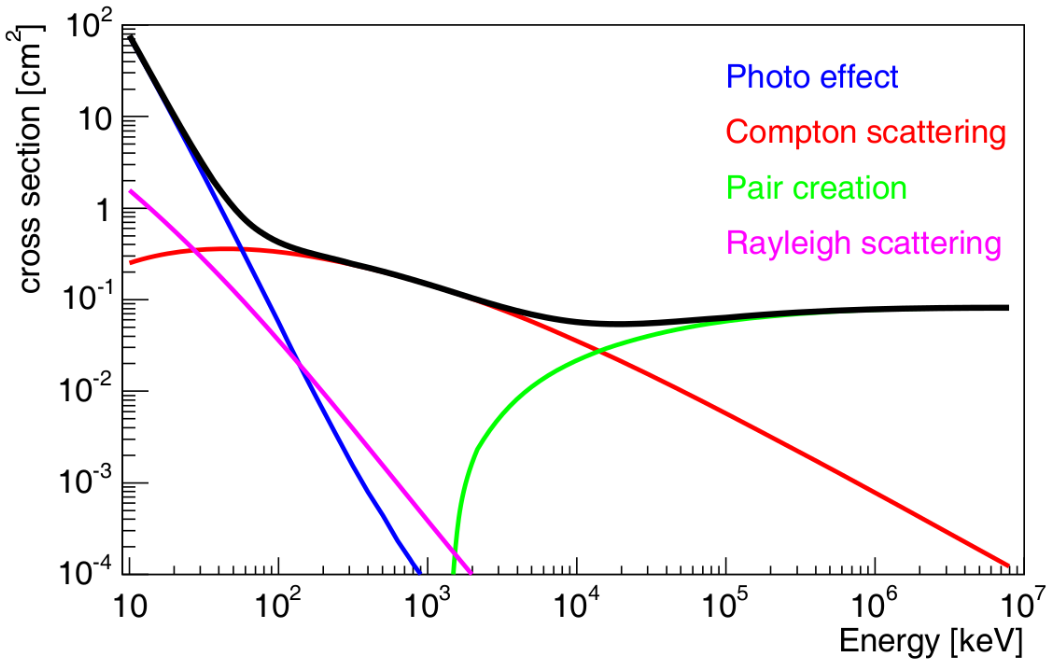
\includegraphics[width=0.2\textwidth]{./fig/photos/cross_stat.png}
    \label{fig:aaaaaa}
  }
  \subfloat[\centering Cross section for compton scattering. Source: \cite{zoglauer}] {

    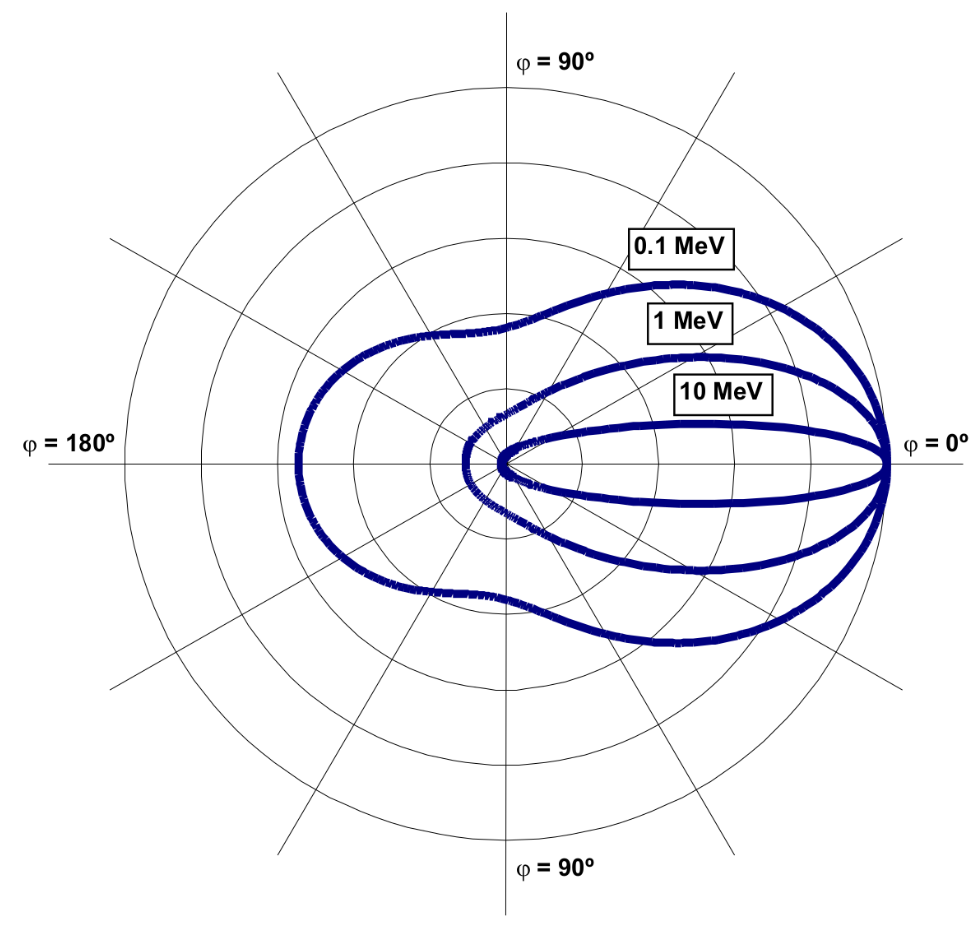
\includegraphics[width=0.2\textwidth]{./fig/photos/cross_section.png}
    \label{fig:aaaaaa}
  }
  \caption{TODO}
  \label{fig:xxx}
\end{figure}% %%}
  \section{Radioactive decay}
  Radioactive decay is a process where an unstable atomic nucleus transforms into a lower-energy state.
  During this process, it loses energy by radiation.
  There are three main types of such radiation - alpha, beta and gamma.
  Whereas alpha particles can be stopped by a sheet of paper and beta particles by aluminium shielding, gamma particles can be blocked only using a thick block of lead or a massive concrete wall.
  Moreover, highly energetic gamma rays have a negative effect on the human body, causing damage on a cellular level.
  Being exposed to such radiation poses a risk of severe health problems or death.

  \section{Some properties of $\gamma$ radiation}
  \subsection{Inverse square law}
  \subsection{Interaction with matter}

  The quantity of emitted particles ("strength" of the source) is expressed in Becquerels.
  It is a SI unit defined as the number of emitted particles per second.

  \section{Interaction with matter}
  As the gamma particle passes through matter, there are three possible effects that might happen:
  \textbf{the photoelectric effect}, \textbf{Compton scattering} and \textbf{pair production}.

  \textbf{The photoelectric effect} is typical at low energies of gamma rays. A photon undergoes an interaction with an electron that is bound in an atom. The incident photon completely disappears in this interaction. A product of this interaction is a photon.
  \textbf{The Compton effect} is typical for mid-energetic gamma rays. In this process, an incident gamma photon loses energy to an atomic electron. A new lower energetic photon is emitted in a different direction (hence the frequently used term "Compton scattering").
  \textbf{Pair production} is typical for high-energetic gamma rays. It is a process in which a photon of sufficient energy is converted into an electron and a positron.

  The Compton effect (published in 1923 \cite{}) describes the way how a (gamma or X-ray) photon interacts with a static electron. An incident photon with wavelength $\lambda$ losses some energy to the electron. A new lower energetic photon with wavelength $\lambda^{\prime}$ is emitted under angle $\beta$. Thanks to the law of conservation of energy and momentum, Compton derived the following equation
  \begin{equation}
      \lambda^{\prime} = \lambda + \frac{h}{m_{e}c}(1-\mathrm{cos} \beta),
  \end{equation}
  where $\lambda$ is the wavelength of the incident photon, $\lambda^{\prime}$ is the wavelength of the emitted photon, $h$ is the Planck constant, $m_{e}$ is the electron rest mass, $c$ is the speed of light and $\beta$ is the scattering angle.

  \begin{figure}[!h]
      \centering
      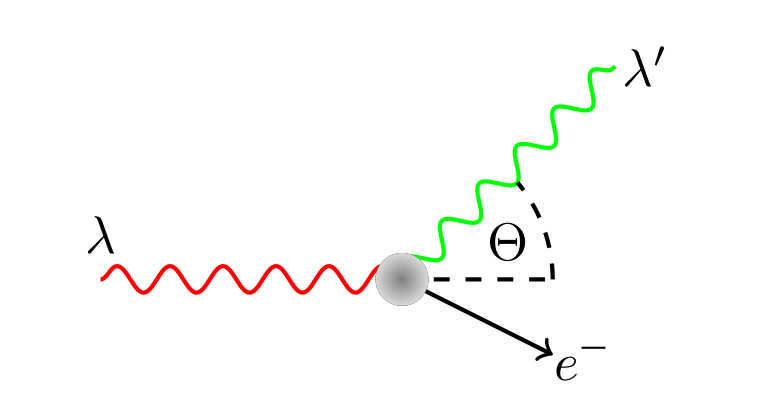
\includegraphics[width=0.3\textwidth]{./fig/photos/scattering.png}
      %\label{fig:scattering}
      %\caption{An illustration of Compton scattering. The incident photon interacts with the static electron. As a result, a new lower energetic photon is emitted in a direction changed by $\beta$ as part of its energy is transferred to electron $e^{-}$. Source: \cite{baca2021gamma}}
  \end{figure}


  \subsection{Klein Nishina formula}
  TODO

  \subsection{Compton effect}
  TODO


  \section{Compton camera}
  This effect is the fundamental principle in a sensor called a Compton camera. 
  The sensor is typically composed of two main components: the scatterer and the absorber. 
  The incident photon first interacts with the scatterer, where the lower energetic photon is emitted under angle $\beta$ (thanks to the Compton effect). 
  Since it is more common to measure energies instead of wavelength, we can rewrite the Compton formula as
  \begin{equation}
  E_{\lambda^{\prime}} = \frac{E_{\lambda}}{  1 + (E_{\lambda} / m_{e}c^{2}) (1 - \mathrm{cos} \beta)},
  \end{equation}
  where $E_{\lambda}$ is the energy of the incoming photon from the source, $E_{\lambda^{\prime}}$ is the energy of the scattered photon.  
  The bi-product of the interaction (electron $e_{e^{-}}$) is immediately measured in the scatterer, and its position is recorded.
  Then, the scattered lower energetic photon interacts with the second layer of the sensor - the absorber. 
  The photoelectric effect is witnessed while measuring the product of it - the energy of the electron $e_{\lambda^{prime}}$ and its position on the absorber.

  Now we can express the scattering angle $\beta$ as
  \begin{equation}
      \beta = \mathrm{arccos} \left (  1-\frac{m_{e}c^{2}E_{\lambda^{\prime}}}{E_{\lambda} (E_{\lambda} - E_{\lambda^{\prime}})} \right )
      %\label{eq:compton_beta_formula}
  \end{equation}

  Given the measurements on the scatterer and absorber and computed scattering angle $\beta$ using the equation \ref{eq:theta} (using known energy of the incoming photon $E_{\lambda}$), we can reconstruct a set of possible directions from where the original photon arrived. Since the Compton effect is symmetrical, the set of possible directions towards the source of ionizing radiation forms a surface of a cone.



  \subsection{MiniPIX TPX3 sensor}
  The sensor used in this work is a small CdTe event-based camera that is capable of witnessing the interactions between gamma photons and the matter of the sensor and reporting them in real time.
  Unlike the traditional model of the Compton camera mentioned before, this is a single-stack detector.
  In other words, there is no distinction between the scatterer and the absorber and all the measurable interactions are happening in one 14x14x2 mm block of CdTe semiconductor material.
  The sensor is capable of measuring a 3D position of the interactions (and distinguishing its type) inside the detector with nanosecond resolution. 
  All these features open the possibility of using it in Compton camera mode.
  Technical details of the sensor are described in \cite{baca2021gamma} and \cite{baca2019timepix}.
  The biggest advantage of this sensor is its small size, low weight and low power consumption.
  Thanks to that, we can use this sensor on board a small UAV. 


  \section{Cs137}

  \section{ROS}

  \section{MRS UAV system}
}
% %%}

%!TEX root = ../main.tex

\chapter{Methods\label{chap:methods}}

\section{Mapping sources of radiation}


\subsection{List-mode Maximum Likelihood Expectation Maximization}

The mapped area is sampled into small bins, indexed as 
\begin{equation}

m_{j} = 1 ... J

\end{equation}





%% --------------------------------------------------------------
%% |                How to write thesis in LaTeX                |
%% --------------------------------------------------------------

%%!TEX root = ../main.tex

\chapter{How to write thesis in LaTeX\label{chap:how_to}}

\section{Versioning with git}

Write the LaTeX in such a way that it could be versioned by git, which will help when collaborating with other people.
This means writing \textbf{one sentence per line}.
Even when you use third-party platforms, such as the OverLeaf, you can still share the repository through Git.

\section{Mathematical notation with LaTeX}

Use bold to visually distinguish vectors and matrices ($\mathbf{x}$, $\mathbf{A}$) and scalars ($k$, $N$).
Mathematical equations should be numbered and should be part of a sentence.
For example, the following equation is a discrete LTI system update
\begin{equation}
  \mathbf{x}_{\left[k+1\right]} = \mathbf{A}\mathbf{x}_k + \mathbf{B}\mathbf{u}_k,
  \label{eq:lti_system}
\end{equation}
where $\mathbf{x}_k \in \mathbb{R}^m$ is the state vector at the sample $k$, $\mathbf{u}_k \in \mathbb{R}^n$ is the input vector, $\mathbf{A} \in \mathbb{R}^{m \times m}$ is the main system matrix, and $\mathbf{B} \in \mathbb{R}^{m \times n}$ is the system input matrix.
Proper punctuation should be used after \refeq{eq:lti_system}, as if it were an ordinary object in the sentence.
Do not put any empty lines around the equation.
That would create a new paragraph mid-sentence.

\section{Using footnotes}

Do not be afraid to use footnotes for additional information, such as http links\footnote{This repository: \url{https://github.com/ctu-mrs/thesis_template}.}.
We use footnote links whenever we want to \emph{point} to a website, rather then to cite it as a source.
Like with everything, do not overdo it.

\section{Referencing to document elements}

LaTeX allows you to dynamically reference to parts of the documents, such as
\begin{itemize}
  \item figures: \reffig{fig:uavs}, Figure\,\ref{fig:uavs},
  \item equations: \refeq{eq:lti_system},
  \item code: \reflst{lst:references},
  \item and any other object that can contain \texttt{label}.
\end{itemize}

Check the section in the \texttt{document\_setup.tex} that contains useful macros for unifying the references:

\begin{lstlisting}[caption={LaTeX macros for referencing to document elements.},label={lst:references}]
  \newcommand{\reffig}[1]{Fig.~\ref{#1}}
  \newcommand{\reflst}[1]{Lst.~\ref{#1}}
  \newcommand{\refalg}[1]{Alg.~\ref{#1}}
  \newcommand{\refsec}[1]{Sec.~\ref{#1}}
  \newcommand{\reftab}[1]{Table~\ref{#1}}
  \newcommand{\refeq}[1]{\eqref{#1}}
\end{lstlisting}

\section{Abbreviations with Acronym}

Abbreviations are handled by the \emph{acronym} package.
Example sentence with abbreviations: ``\ac{UAV} is a flying vehicle that commonly uses \ac{LiDAR} and \ac{GPS} receiver''.
Please, read the documentation\footnote{Acronym package: \url{http://mirrors.ctan.org/macros/latex/contrib/acronym/acronym.pdf}}.

\section{Units of measurements with Siunitx}

Typesetting of units has never been more accessible with the Siunitx package.
Acceleration is measure in \si{\meter\per\second\squared}.
Gravity accelerates objects at a rate $\approx \SI{9.81}{\meter\per\second\squared}$ near the sea level.
You can define your units if you want.

Becquerel: $ \SI{10}{\mega\becquerel} $

\section{2D Diagrams with Tikz}

\emph{Tikz} is a powerful tool for drawing 2D (and 3D) shapes and diagrams.
Check the documentation and examples: \url{https://www.overleaf.com/learn/latex/TikZ_package}.
The benefit of using \emph{Tikz}, instead of some other third-party drawing program, are:
\begin{itemize}
  \item fonts are the same as in LaTeX,
  \item you can typeset math in LaTeX,
  \item you can use references to other parts of your document,
  \item you can version the image in git,
  \item the images are easily adjustable while editing your document.
\end{itemize}
Check \reffig{fig:pgfplots} for example.

\begin{figure}[!h]
  \centering

  \begin{adjustbox}{max totalsize={0.6\textwidth}{0.90\textheight}, center}
    \tikzset{
  >=stealth',
  punkt/.style={
    rectangle,
    rounded corners,
    draw=black, very thick,
    text width=5.7em,
    minimum height=2em,
    text centered,
  },
  small_punkt/.style={
    rectangle,
    rounded corners,
    draw=black, very thick,
    text width=4.0em,
    text centered,
  },
  arrow/.style={
    ->,
    very thick,
    shorten <=2pt,
    shorten >=2pt,
  },
  arrow_red/.style={
    ->,
    draw=red, very thick,
    shorten <=2pt,
    shorten >=2pt,
  },
}

\begin{tikzpicture}[node distance=1cm, auto,]

  % outer circle nodes
  \node[punkt] (sensor) {Sensor size};
  \node[punkt, inner sep=5pt, below = of sensor, shift = {(-6.0, -0.75)}] (aircraft) {Aircraft\\size};
  \node[punkt, inner sep=5pt, below = of sensor, shift = {(0.0, -4.0)}] (constraints) {Environment constraints};
  \node[punkt, inner sep=5pt, below = of sensor, shift = {(6.0, -0.75)}] (strategy) {Localization strategy};

  % inner circle nodes
  \node[small_punkt, inner sep=5pt, below = of sensor, shift = {(0.0, 0.5)}] (sensor2) {\scriptsize Sensor size};
  \node[small_punkt, inner sep=5pt, right = of aircraft, shift = {(0.5, -0.0)}] (aircraft2) {\scriptsize Aircraft\\size};
  \node[small_punkt, inner sep=5pt, above = of constraints, shift = {(0.0, -0.5)}] (constraints2) {\scriptsize Environment\\constraints};
  \node[small_punkt, inner sep=5pt, left = of strategy, shift = {(-0.5, -0.0)}] (strategy2) {\scriptsize Localization\\strategy};

  \path[->] ($(sensor.west)+(0, 0)$) edge [arrow,bend right=45] ($(aircraft.north)$);
  \path[->] ($(aircraft.south)+(0, 0)$) edge [arrow,bend right=45] ($(constraints.west)$);
  \path[->] ($(constraints.east)+(0, 0)$) edge [arrow,bend right=45] ($(strategy.south)$);
  \path[->] ($(strategy.north)+(0, 0)$) edge [arrow,bend right=45] ($(sensor.east)$);

  % inner circle paths
  \path[->] ($(sensor2.west)+(0, 0)$) edge [arrow_red, bend right=45, dashed] ($(aircraft2.north)+(0.0, 0.0)$);
  \path[->] ($(aircraft2.south)+(0, 0)$) edge [arrow_red, bend right=45, dashed] ($(constraints2.west)+(0.0, 0.0)$);
  \path[->] ($(constraints2.east)+(0, 0)$) edge [arrow_red, bend right=45, dashed] ($(strategy2.south)+(0.0, 0.0)$);
  \path[->] ($(strategy2.north)+(0, 0)$) edge [arrow_red, bend right=45, dashed] ($(sensor2.east)+(0.0, 0.0)$);

  % outer inner arrows
  \draw [->] ($(sensor.south)+(0, 0)$) -- ($(sensor2.north)$) node [midway, shift = {(0.0, 0.0em)}] {smaller};
  \draw [->] ($(aircraft.east)+(0, 0)$) -- ($(aircraft2.west)+(0.0, 0.0)$) node [midway, shift = {(0.0, 0.0em)}] {smaller};
  \draw [->] ($(constraints.north)+(0, 0)$) -- ($(constraints2.south)+(0.0, 0.0)$) node [midway, shift = {(0.0, 0.0em)}] {more complex};
  \draw [->] ($(strategy.west)+(0, 0)$) -- ($(strategy2.east)+(0.0, 0.0)$) node [midway, shift = {(0.0, 0.0em)}] {smarter};

\end{tikzpicture}

  \end{adjustbox}

  \caption{Example of a 2D diagram using tikz \emph{PGFPlots}.}
  \label{fig:pgfplots}
\end{figure}

\section{Data plots with PGFPlots}

\emph{PGFPlots} produces nice 2D and 3D data plots from data stored in CSV.
The plot parameters can be versioned and easily adjusted by editing the plot definition file.
\begin{itemize}
  \item Documentation and manual: \url{https://ctan.org/pkg/pgfplots}
  \item Compile the plots individually and then include the pdfs because it can take longer.
  \item Example located in \texttt{fig/plots/example\_plot}, see \reffig{fig:pgfplots}.
  \item You could include the latex file directly. However, it will take longer to compile, and platforms such as Overleaf can have a problem with that.
\end{itemize}

\begin{figure}[!h]
  \centering
  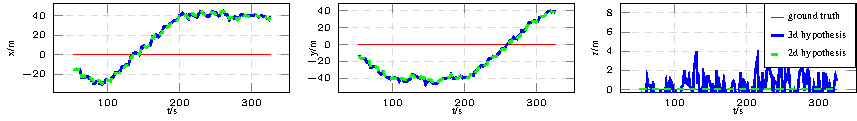
\includegraphics[width=1.0\textwidth]{./fig/plots/example_plot/hypotheses.pdf}
  \caption{Example of a 2D plot using \emph{PGFPlots}.}
  \label{fig:pgfplots}
\end{figure}

\section{3D Plots with Sketch}

\emph{Sketch} is a tool for defining a 3D scene using simple descriptive language.
The 3D scene is then converted to \emph{Tikz}, which is later compiled to pdf.
The benefits of using \emph{Sketch} are similar to using \emph{Tikz}: LaTeX fonts, versioning using git, and cleanness of the result.
See the example image in \reffig{fig:coordinate_systems}.
\begin{itemize}
  \item Documentation and manual: \url{http://www.frontiernet.net/~eugene.ressler/}
  \item Cross-compilation from \emph{Sketch} to \emph{pdf} using the \texttt{fig/sketch/compile\_sketch.sh} script.
\end{itemize}

\begin{figure}[!h]
  \centering
  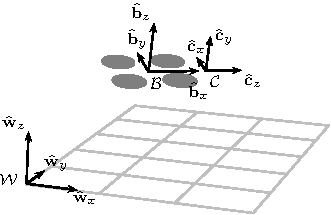
\includegraphics[width=0.4\textwidth]{./fig/sketch/coordinate_frames.pdf}
  \caption{Depiction of the used coordinate systems. The image was drawn using \emph{Sketch}.}
  \label{fig:coordinate_systems}
\end{figure}

\section{Image collages with Subfig}

We recommend using the \emph{subfig} packages, which provides the \emph{subfloat} command.
It is more versatile than the simpler \emph{subcaption} package.
Check the \reffig{fig:uavs} for example.

\begin{figure}[!h]
  \centering
  \subfloat[A UAV, the T650 model.] {
    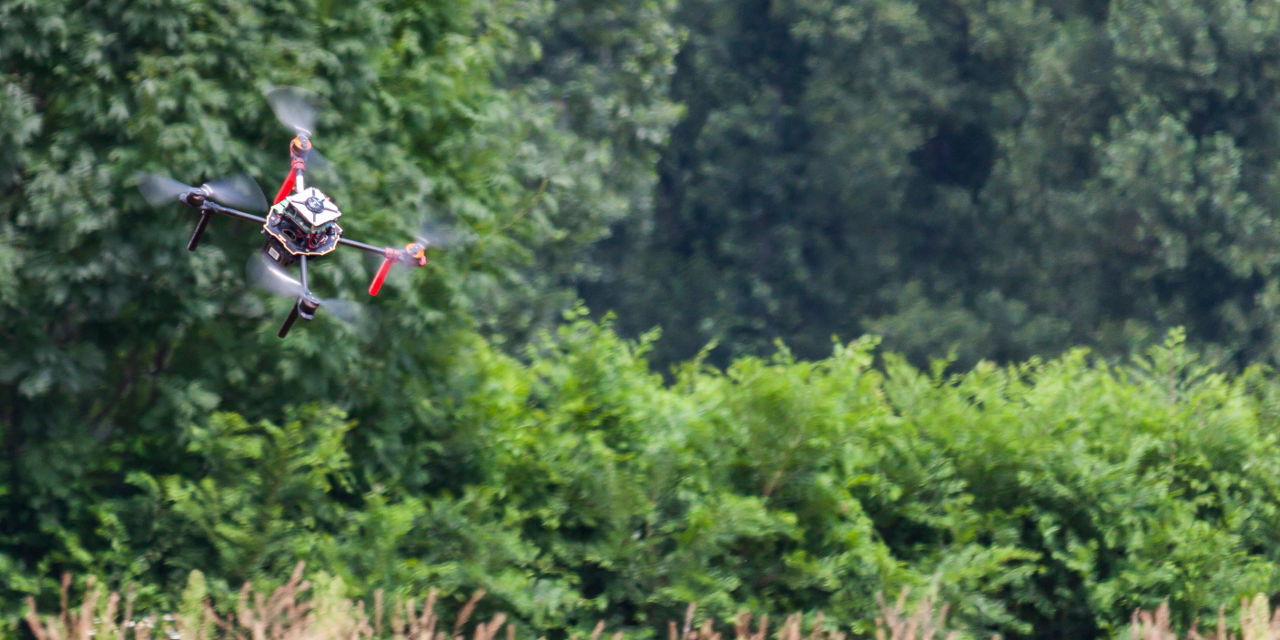
\includegraphics[width=0.48\textwidth]{./fig/photos/uav1.jpg}
    \label{fig:uavs_1}
  }
  \subfloat[Another UAV, again, T650 model.] {
    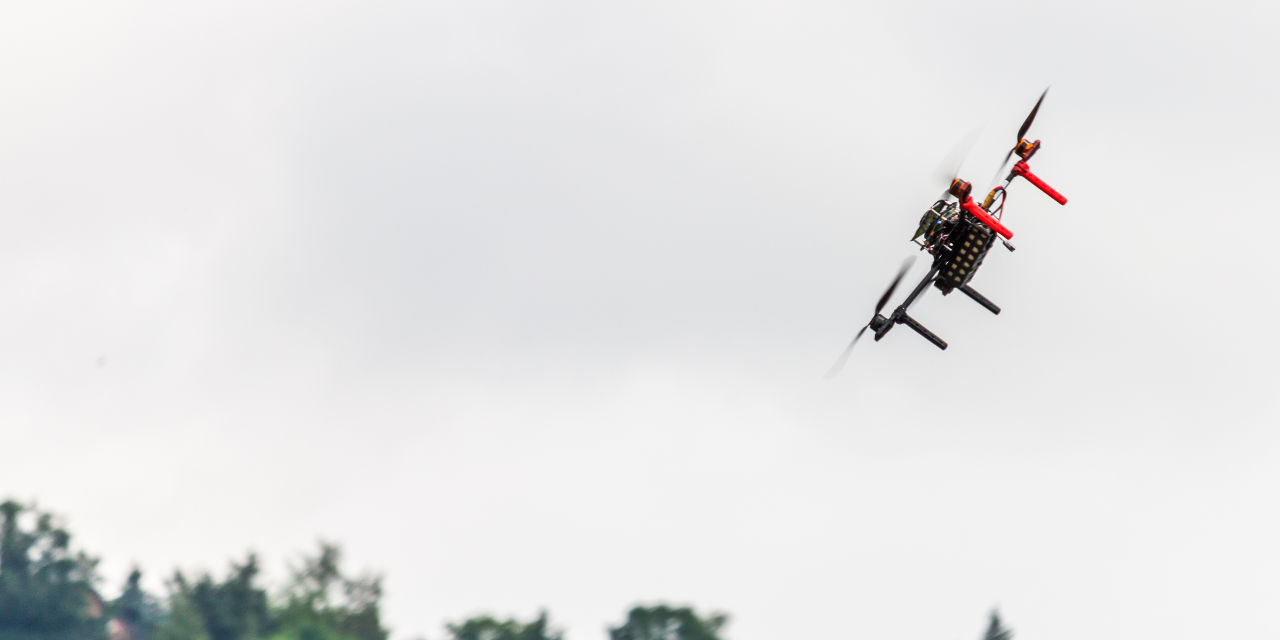
\includegraphics[width=0.48\textwidth]{./fig/photos/uav2.jpg}
    \label{fig:uavs_2}
  }
  \caption{The caption should mention both, the \reffig{fig:uavs_1} and the \reffig{fig:uavs_2}. You can just refer to them as (a) and (b), but beware, you need to keep it correct as you edit.}
  \label{fig:uavs}
\end{figure}

\section{Citations with Biblatex}

\emph{Biblatex} is probably the most powerful citation package for LaTeX.
It consumes the standard \texttt{.bib} file. However, it can sort and filter the citations using the \texttt{keywords} tag.
%Citing references is done using the \texttt{cite} command, e.g., \cite{baca2021mrs}.
You can also define some nice citation boxes, such as this one:
%\fullciteinbox{baca2021mrs}{}

\section{Image overlays with Tikz}

\emph{Tikz} is very useful to create custom image overlays.
The overlay can be set such that the image is spanned by Cartesian coordinates $\left(x, y\right) \in \left[0, 1\right]^2$
Example can be seen in \reffig{fig:tikz_overlay}.

\begin{figure}[!h]

  \centering

  \subfloat {\begin{tikzpicture}
    \node[anchor=south west,inner sep=0] (a) at (0,0) { 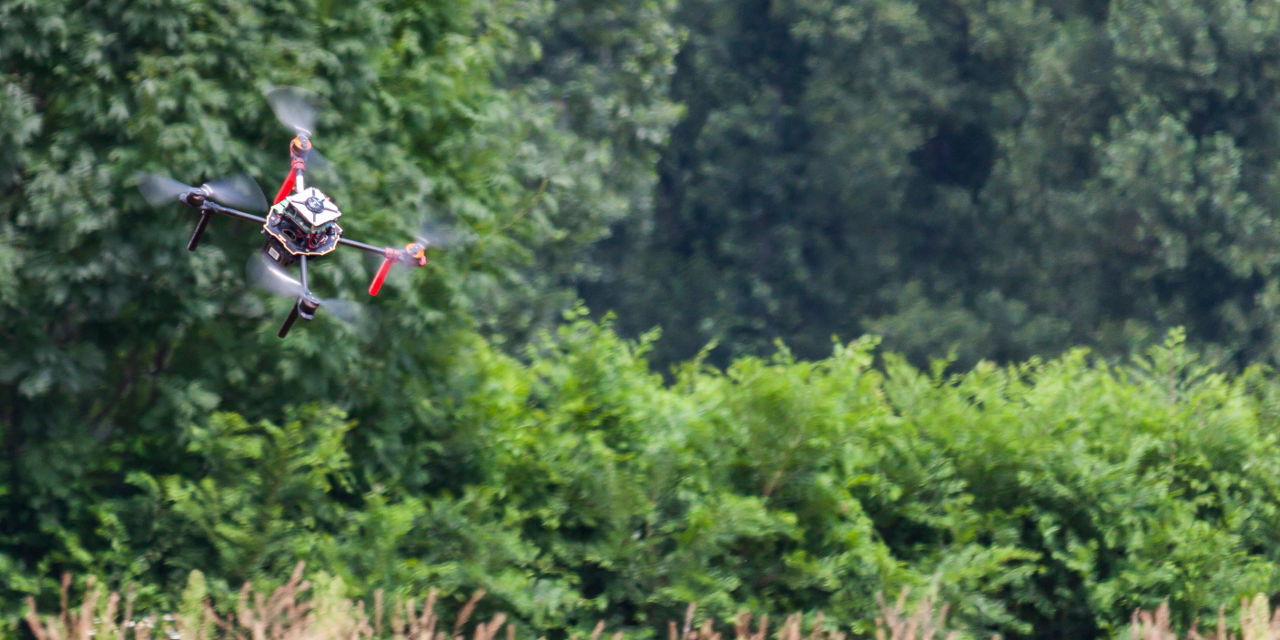
\includegraphics[width=0.45\textwidth]{./fig/photos/uav1.jpg}};
    \begin{scope}[x={(a.south east)},y={(a.north west)}]

      %%{ grid for placing the elements

      % % useful grid to help you find coordinates for plotting the overlay
      % \draw[black, xstep=.1, ystep=.1] (0,0) grid (1,1);
      % \foreach \i in {0,0.1,0.2,0.3,0.4,0.5,0.6,0.7,0.8,0.9,1} {
      %   \node[align=center] at (\i, -0.05) {\i};
      %   \node[align=center] at (\i, 1.05) {\i};
      %   \node[align=center] at (-0.05, \i) {\i};
      %   \node[align=center] at (1.05, \i) {\i};
      % }

      %%}

      % plot some stuff over the image

      % plot white background behind the letter (a)
      \fill[white] (0.001, 0.001) rectangle (0.08,0.14);

      % plot black border
      \fill[draw=black, draw opacity=0.5, fill opacity=0] (0,0) rectangle (1, 1);

      % write the letter (a) in the bottom-left corner
      \draw (0.04,0.06) node [text=black] {\small (a)};

      % plot black border
      \draw[->, white, thick] (0.50, 0.80) -- (0.30, 0.67);
      \draw (0.50,0.86) node [text=white] {\small \textbf{UAV}};
    \end{scope}
  \end{tikzpicture}}
\hfill%
\subfloat {\begin{tikzpicture}
    \node[anchor=south west,inner sep=0] (a) at (0,0) { 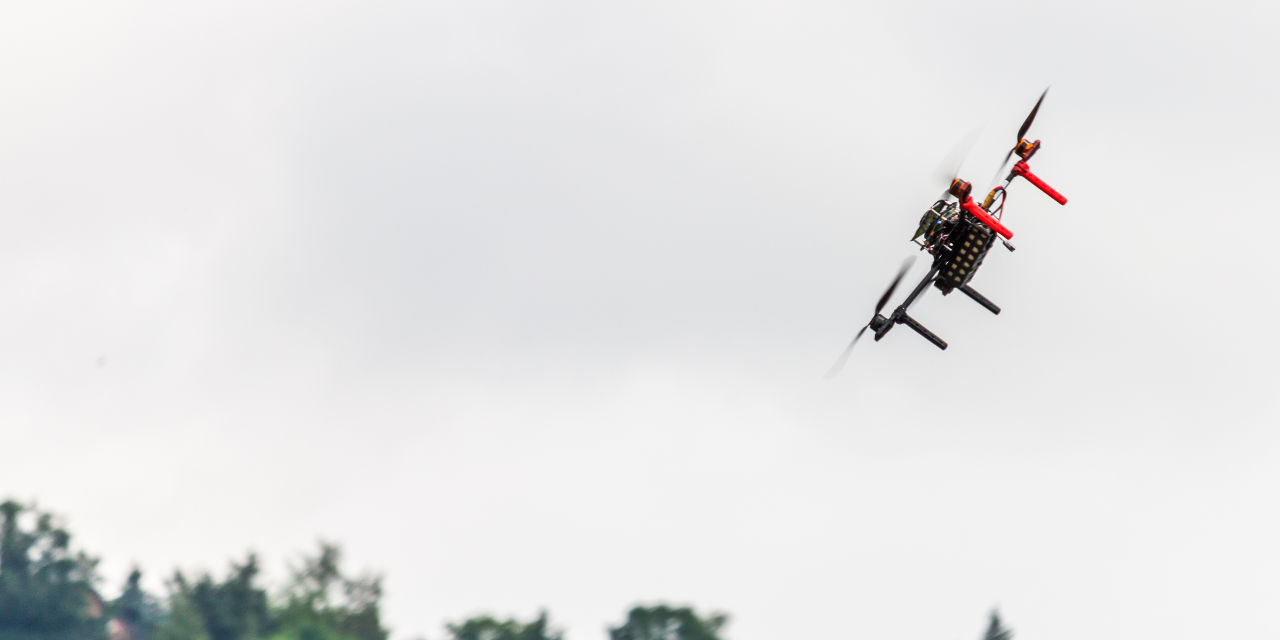
\includegraphics[width=0.45\textwidth]{./fig/photos/uav2.jpg}};
    \begin{scope}[x={(a.south east)},y={(a.north west)}]

      %%{ grid for placing the elements

      % useful grid to help you find coordinates for plotting the overlay
      \draw[black, xstep=.1, ystep=.1] (0,0) grid (1,1);
      \foreach \i in {0,0.1,0.2,0.3,0.4,0.5,0.6,0.7,0.8,0.9,1} {
        \node[align=center] at (\i, -0.05) {\i};
        \node[align=center] at (\i, 1.05) {\i};
        \node[align=center] at (-0.05, \i) {\i};
        \node[align=center] at (1.05, \i) {\i};
      }

      %%}

      % plot some stuff over the image

      % plot white background behind the letter (b)
      \fill[white] (0.001, 0.001) rectangle (0.08,0.14);

      % plot black border
      \fill[draw=black, draw opacity=0.5, fill opacity=0] (0,0) rectangle (1, 1);

      % write the letter (b) in the bottom-left corner
      \draw (0.04,0.06) node [text=black] {\small (b)};
    \end{scope}
  \end{tikzpicture}}


  \caption{Example of using Tikz for image overlays. (a) shows a final product, (b) shows a grid useful for nailing down the coordinates.}
  \label{fig:tikz_overlay}

\end{figure}


%!TEX root = ../main.tex

\chapter{Results\label{chap:results}}
This chapter demonstrates the functionality of the proposed method\footnote{Videos from the experiments are available here: \url{http://mrs.felk.cvut.cz/theses/werner2023thesis}} for the localization of sources of ionizing radiation and its individual components.
Unfortunately, it was not possible to test the proposed methods using real sources of ionizing radiation for organizational reasons, since the use of radioactive materials is strictly regulated and requires coordination with state authorities (National Institute for Nuclear, Chemical and Biological Protection) and manufacturer of the \ac{pix}.
%That results in the fact that most of recorded data from real world experiments cant be used because the drones simply did not come close enough to other sources and 
Another problem is the absence of methods for comparison, that would be a) available, b) capable of localization of multiple sources using the Compton camera measurements.
Therefore we use the back-projection reconstruction method (described in Chapter \ref{chap:mlem_theory}) as a baseline.
This chapter presents results of the Monte Carlo simulation (Section \ref{chap:mcr}), 
performance of the system on recorded real-world data (Section \ref{chap:exp1}), 
in simulation (Section \ref{chap:exp2}) and in real-world experiment with simulated data (Section \ref{chap:exp3}). 
%The directional sensitivity of the \ac{pix} sensor, modelled via Monte Carlo simulation, is presented in \autoref{chap:mcr}.
%The evaluation of the \ac{MLEM} estimation approach, carried out on previously gathered data from experiments with real radioactive sources, is shown in \autoref{chap:exp1}.
%The functionality of the whole system (estimation method together with the proposed search strategy) in simulation is presented in \autoref{chap:exp2}.
%Finally, the whole system was also tested on real hardware with simulated radioactive sources, as shown in \autoref{chap:exp3}.

\section{Monte Carlo simulation of the sensor's sensitivity\label{chap:mcr}}
The assessment of the directional sensitivity of the \ac{pix} sensor was carried out using the Monte Carlo simulation described in Chapter \ref{chap:methods_estimation}.
Each omnidirectional simulated source (located $\SI{1}{\meter}$ from the sensor) emitted $10^{10}$ $\SI{662}{\kilo\electronvolt}$ photons from each position.
Shortly speaking, the simulator recorded the number of photons that a) reached the sensor's surface (more precisely, the \ac{CdTe} block, where the ionizing particles interact with \ac{CdTe} material) and b) undergone the interactions (Compton scattering, photoelectric absorption) leading to the Compton cone detection.  
Results of the Monte Carlo simulations are shown in \autoref{fig:monte_clar}.
The corresponding geometry of the \ac{CdTe} block is shown in \autoref{fig:monte_axes}.

The \ac{pix} sensor's directional sensitivity is depicted in \autoref{fig:monte_finalll}.
It can be observed that the probability of a particle being detected as a Compton event is nearly the same from all directions (more precisely, it varies from $3.79 \times 10^{-8}$ to $5.15\times 10^{-8}$).
The probability of reaching the sensor's surface (given the solid angle of the sensor from different positions) is shown in \autoref{fig:monte_reaching}.
A particle emitted in front of the sensor (along the x-axis) is more likely to hit the \ac{CdTe} block than another one emitted from the side (y-axis and z-axis), where the visible surface of the \ac{CdTe} block is the smallest.
On the other hand, the probability of Compton scattering as well as photoelectric absorption (that together lead to the detection of a Compton cone) depend on the trajectory of the incident and scattered photon.
The longer the intersection of an ionizing particle and the \ac{CdTe} block is, the more likely the interactions happen.
Therefore a photon reaching the sensor's surface from the side more likely causes the Compton measurement, as can be seen in \autoref{fig:monte_cone_from_hitting}.
In summary, both effects (probability of reaching the \ac{CdTe} block and probability of necessary interactions) neglect each other and lead to the almost uniform directional sensitivity of the \ac{pix} sensor.
%on the length of the intersection of the photon trajectory with the sensor \ac{CdTe} block.

The absolute values of estimated probabilities and also worth mentioning.
The \ac{pix} sensor with its dimensions $14.08 \times 14.08 \times 2 \ \si{\milli\meter}$ is very small compared to the distance between the \ac{UAV} carrying the sensor and sources of ionizing radiation.
Moreover, approximately only 1 of 100 $\SI{662}{\kilo\electronvolt}$ photons that reach the \ac{pix} sensor can be detected in the Compton camera mode.
For illustration: based on the simulation results, only $\approx 15$ Compton events can be possibly detected (on average) by a \ac{pix} sensor located $\SI{5}{\meter}$ 
from a source of $\SI{662}{\kilo\electronvolt}$ photons  with activity $\SI{1}{\giga\becquerel}$
(assuming exposure time $\SI{10}{\second}$). 
This estimate can be seen as an upper bound since it does not take into account other aspects of the detection process.
For example, other interactions might occur (the incident photon might be immediately absorbed without any Compton scattering), and the detection process might not estimate all the Compton cones correctly due to the noise caused by other particles detected by the Timepix detector at the same time.

% Answer: [trim={left bottom right top},clip]

\begin{figure}[!htb]% %%{
  \subfloat[$p(\mathrm{cone\ detected})$] {
    \centering
    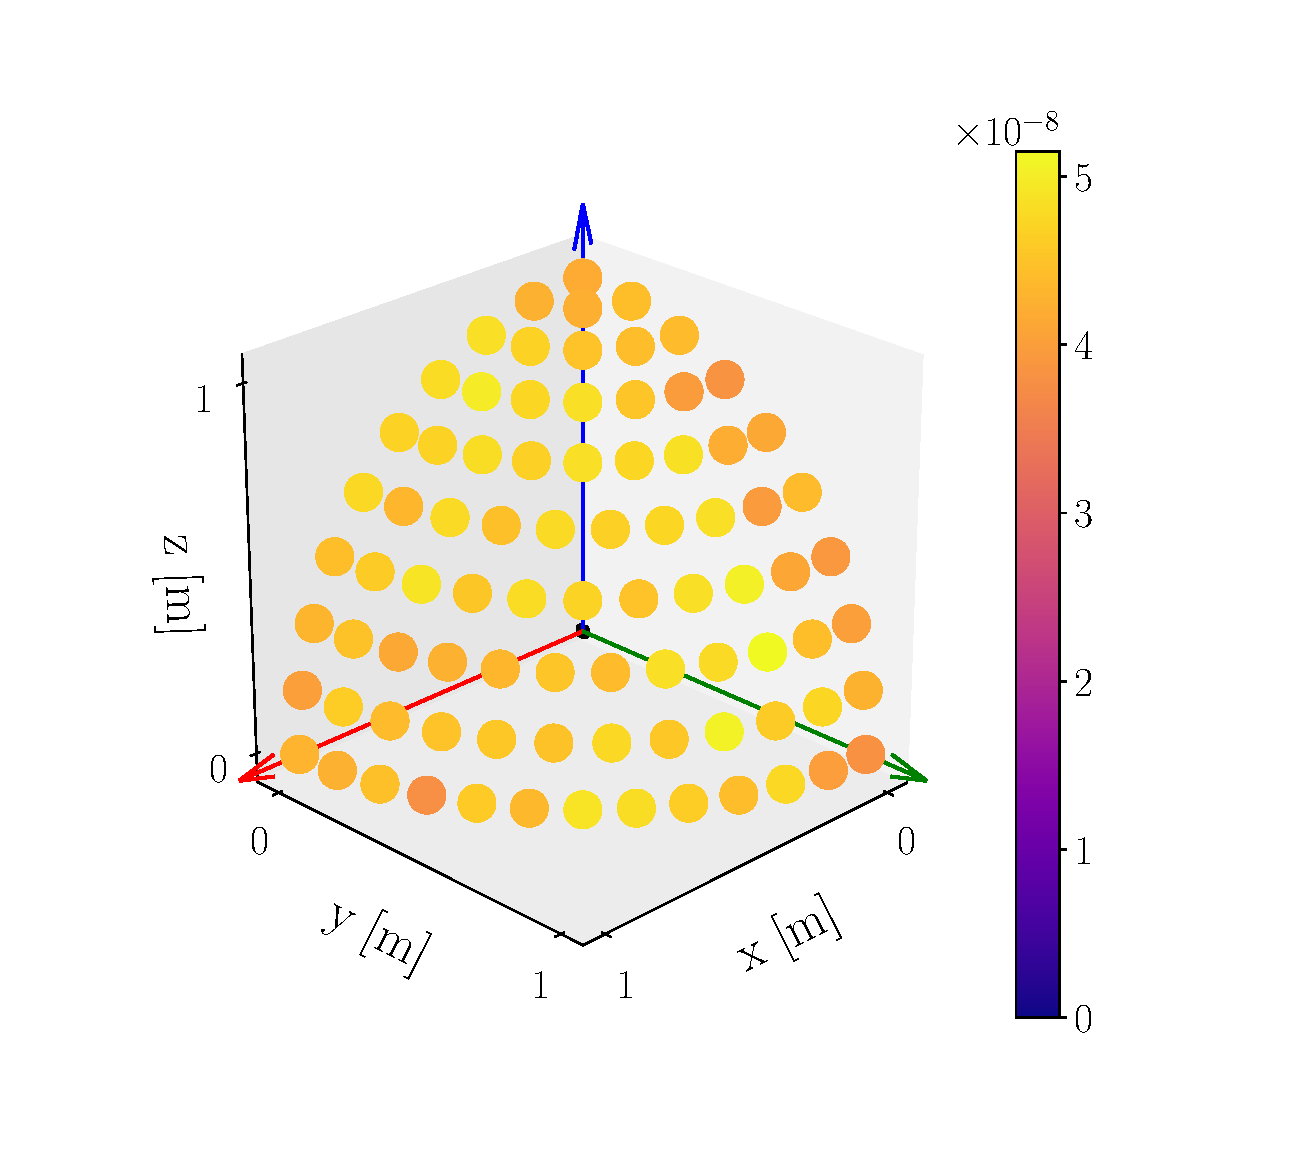
\includegraphics[width=0.42\textwidth,trim={1cm 1cm 2.5cm 1cm},clip]{./fig/photos/monte_carlo_final_prob.eps}
    \label{fig:monte_finalll}
  }
	\centering
  \subfloat[\ac{pix} sensor geometry. The \ac{CdTe} block (grey) has dimensions $14.08 \times 14.08 \times 2 \ \si{\milli\meter}$]{
    \centering
    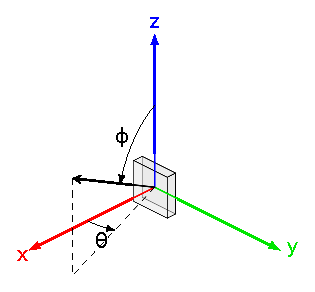
\includegraphics[width=0.4\textwidth]{./fig/photos/axes.eps}
    \label{fig:monte_axes}
  }
  \newline

  \noindent

  \subfloat[$p(\mathrm{reaching\ the\ sensor})$] {
    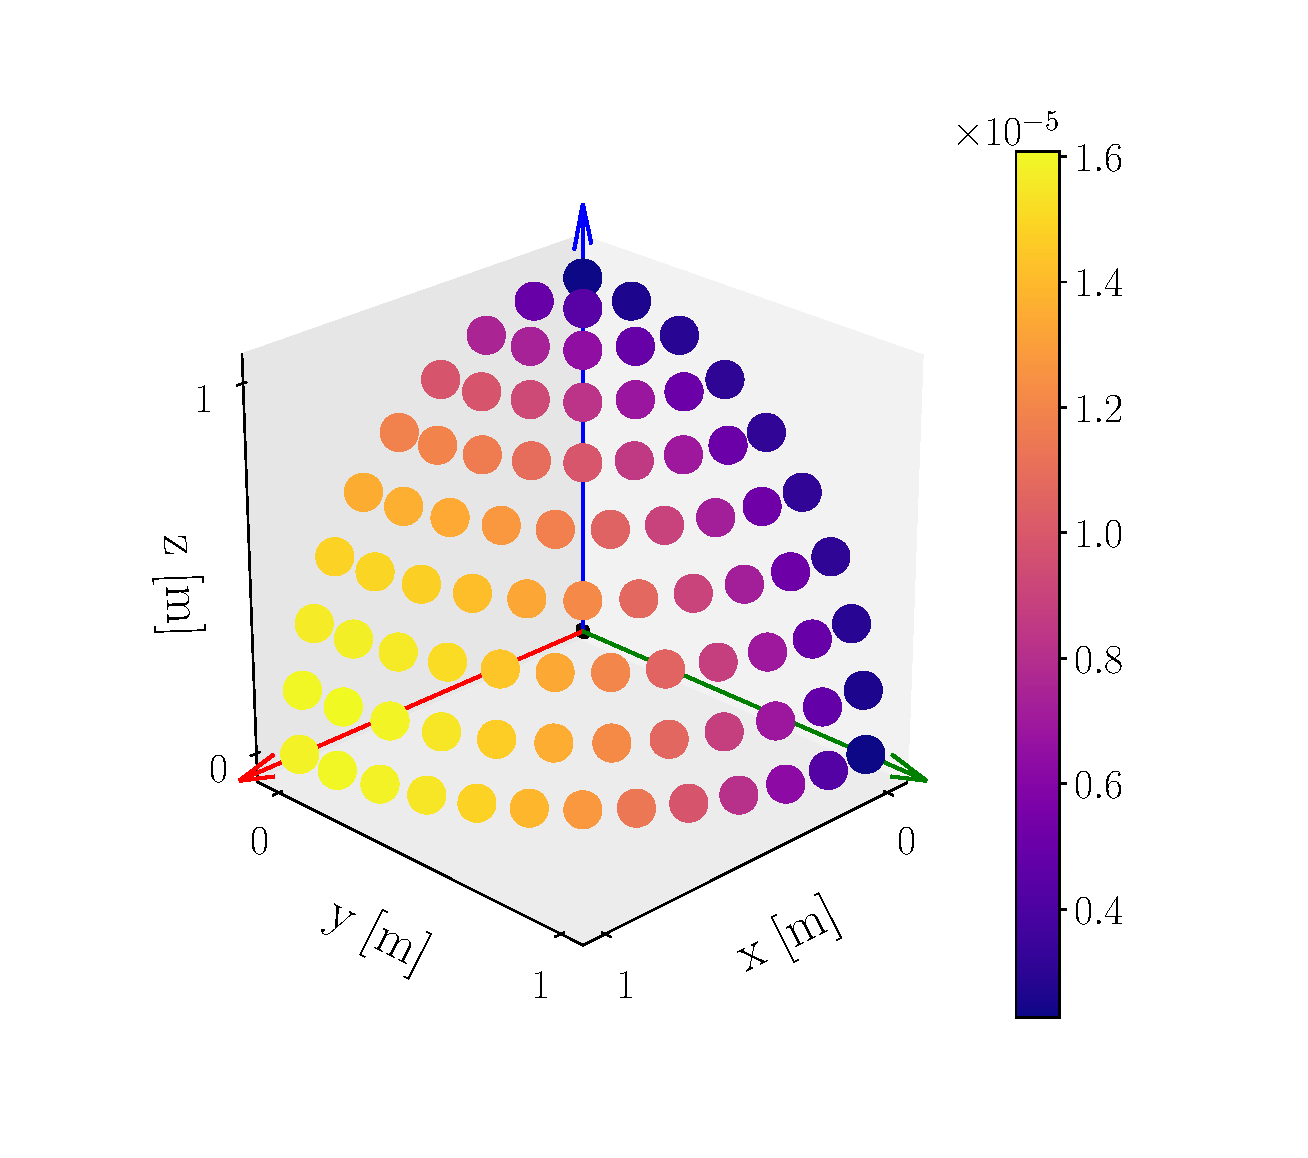
\includegraphics[width=0.42\textwidth,trim={1cm 1cm 1cm 1cm},clip]{./fig/photos/monte_carlo_total_activity.eps}
    \label{fig:monte_reaching}
  }
  \subfloat[$p(\mathrm{cone\ detected}\ |\ \mathrm{reaching\ the\ sensor})$] {
    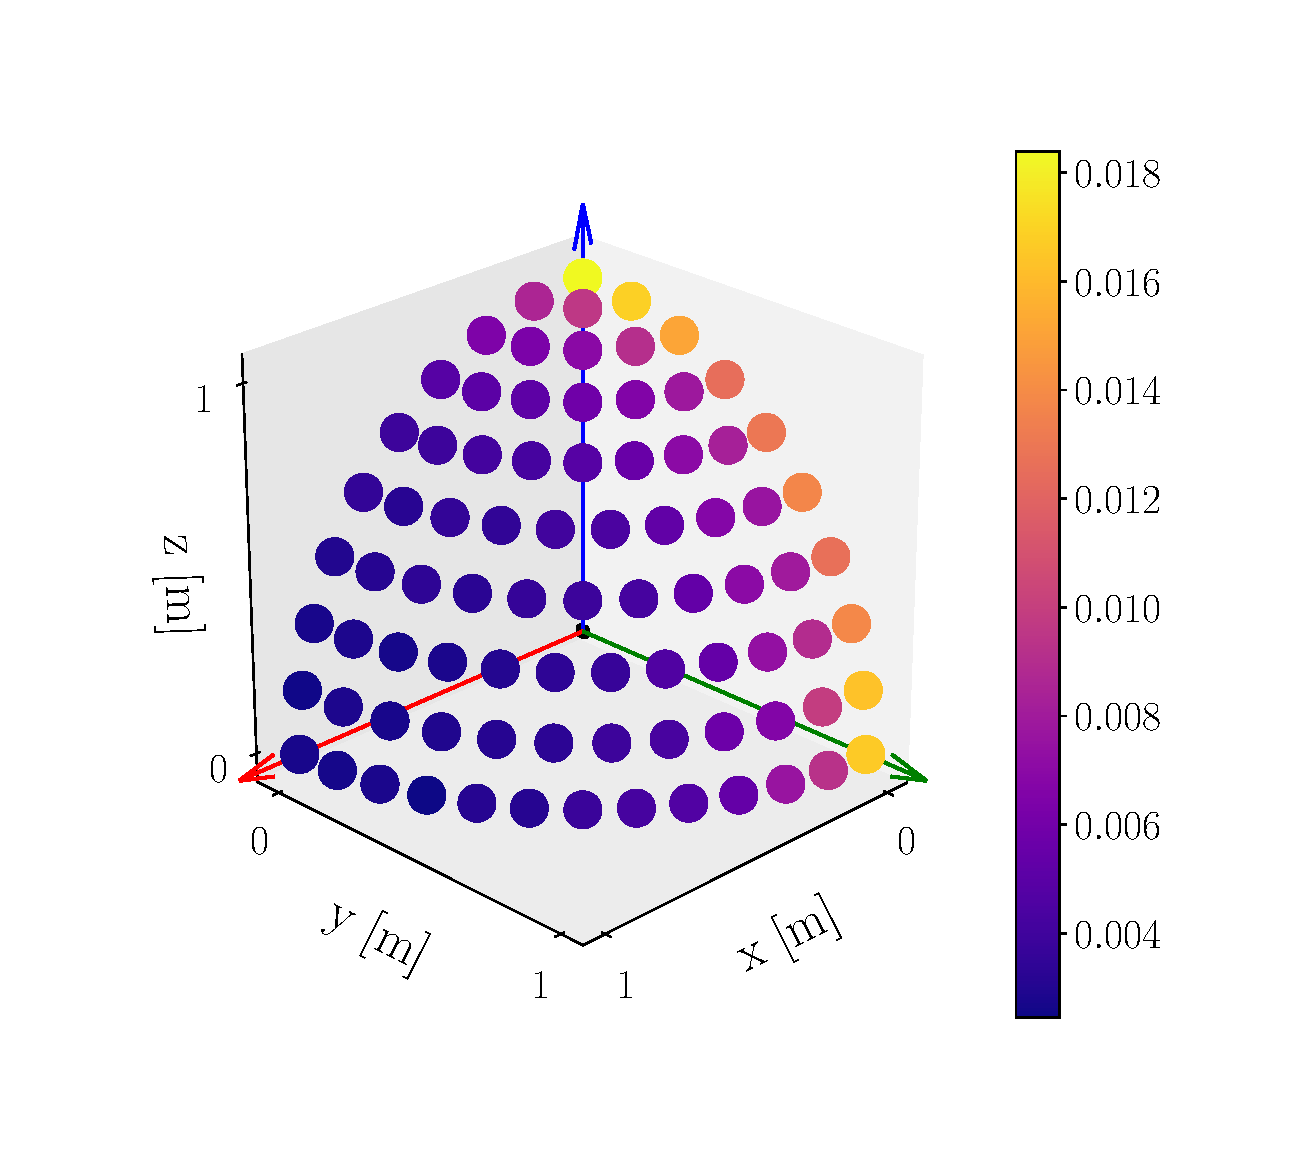
\includegraphics[width=0.42\textwidth,trim={1cm 1cm 1cm 1cm},clip]{./fig/photos/monte_carlo_fraction.eps}
    \label{fig:monte_cone_from_hitting}
  }
  \caption{Direction sensitivity of the \ac{pix} sensor (geometry of the sensor depicted in \protect\subref{fig:monte_axes}). 
  The probability that a $\SI{662}{\kilo\electronvolt}$ photon emitted at the corresponding position causes a Compton cone is depicted in \protect\subref{fig:monte_finalll}. 
  The probability that the particle emitted at a given position reaches the detector is depicted in \protect\subref{fig:monte_reaching}. 
  Lastly, the probability that a photon (that reached the sensor) causes a Compton cone is illustrated in \protect\subref{fig:monte_cone_from_hitting}.}
  \label{fig:monte_clar}
\end{figure}% %%}
%%%%%%%%%%%%%%%%%%%%%%%%%%%%%%%%%%%%%%%%%
\newpage
\section{Evaluation of MLEM method based on real-world data\label{chap:exp1}}
The proposed \ac{MLEM} method for radiation mapping has been tested using data from real-world experiments that were carried out in September 2022 (before the work on this thesis started).
Although the pre-recorded real-world data were collected in realistic conditions with real sensors and sources of ionizing radiation, the prerecorded data do not allow to fully test capabilities of the proposed system.
The reason is the strong dependency between drones trajectories during the experiment and recorded measurements (caused by properties of the ionizing radiation, such as the inverse square law, that is significantly reducing distance from which a radioactive source might be perceived). 
Therefore the outcome of reconstruction strongly depends on in which areas the drones flew during the recorded experiments.

\subsection{Setup and course of the experiment (data collection)}
The area of interest of size $\approx 40 \times 30\ \si{\meter}$ was scanned by a group of four \ac{UAV}s equipped with \ac{pix} sensor.
The \ac{UAV}s were localized using \ac{GPS}.
The drones were controlled by the method proposed in \cite{baca2021gamma}.
In the beginning of the experiment, the drones were following a predefined trajectory covering the whole area of interest uniformly.
After the first 8 Compton cones were detected, three drones were flying $\SI{3}{\meter}$ above the ground encircling the current single-hypothesis estimate of the source position (filtered by a \ac{LKF}). 
The last drone with flight height $\SI{6}{\meter}$ was following a predefined path covering the whole area.
Four sources of Cesium-137 with activity $1900, 500, 180, 50\ \si{\mega\becquerel}$ were located at positions shown in \autoref{e1:gt}.
During the run of the experiment, the drones were mostly encircling the $\SI{500}{\mega\becquerel}$ source position.
The fourth \ac{UAV} flying $\SI{6}{\meter}$ above the ground twice detected photons originating from the $\SI{1900}{\mega\becquerel}$ source. 
As a consequence, the single hypothesis moved towards the strongest source. However, the group of \ac{UAV}s moved back to the $\SI{500}{\mega\becquerel}$ source after a while.
The whole experiment took $\approx \SI{10}{\minute}$, and $263$ Compton cones were recorded.

\subsection{Evaluation of the MLEM method}
The results of the proposed \ac{MLEM} estimation method are presented in \autoref{fig:e1_all}.
The area of interest was discretized with $\SI{1}{\meter}$ resolution, and the number of iterations of the \ac{MLEM} method was set to 10.
The viewpoints (positions of the drones) were sampled with $\SI{5}{\hertz}$, and the \ac{MLEM} estimate was updated every $\SI{2}{\second}$.
The uncertainty of the cone angle  
The final estimate of the emission intensity $\bm{\lambda}$ (based on all data acquired during the experiment) is presented in \autoref{e1:lam}. 
The sensitivity of detection (\autoref{e1:sen}) confirms what was stated before - the drones were mostly encircling the $\SI{500}{\mega\becquerel}$ source at position $(-2, -10)$, which was also correctly localized.
The area in the vicinity of the $\SI{1900}{\mega\becquerel}$ source at position $(16, 0)$ was much less explored by the \ac{UAV}s (and therefore fewer Compton cones originating there were recorded).
Despite the much lower sensitivity in that area, the \ac{MLEM} method estimated some local maxima in the neighbourhood of the true position of the strongest source.
The two weakest sources of radiation are indistinguishable from the noise.



\mycomment{% %%{
  \subsection{Convergence of the MLEM algorithm}
The convergence of \ac{MLEM} algorithm (using \ac{MSE} as the metric) is shown in \autoref{e1:mse}. 
\ac{MSE} in this scenario is defined as
\begin{equation}
MSE = \frac{1}{J} \sum_{j = 0}^{J} (\lambda_{j_{normalized}} - g_{j})^{2},
\end{equation}
where the ground truth is defined as $g_{j} = \frac{\mathrm{source\ activity}}{\mathrm{max}(\mathrm{source\ activity})}$ at the sources locations and $g_{j} = 0$ elsewhere.
The iterative \ac{MLEM} algorithm is initialized with back-projection (\autoref{e1:bp}). 
We can see in \autoref{e1:mse} that the decrease of the $MSE$ stopped after a few iterations.

\begin{figure}
	\centering
    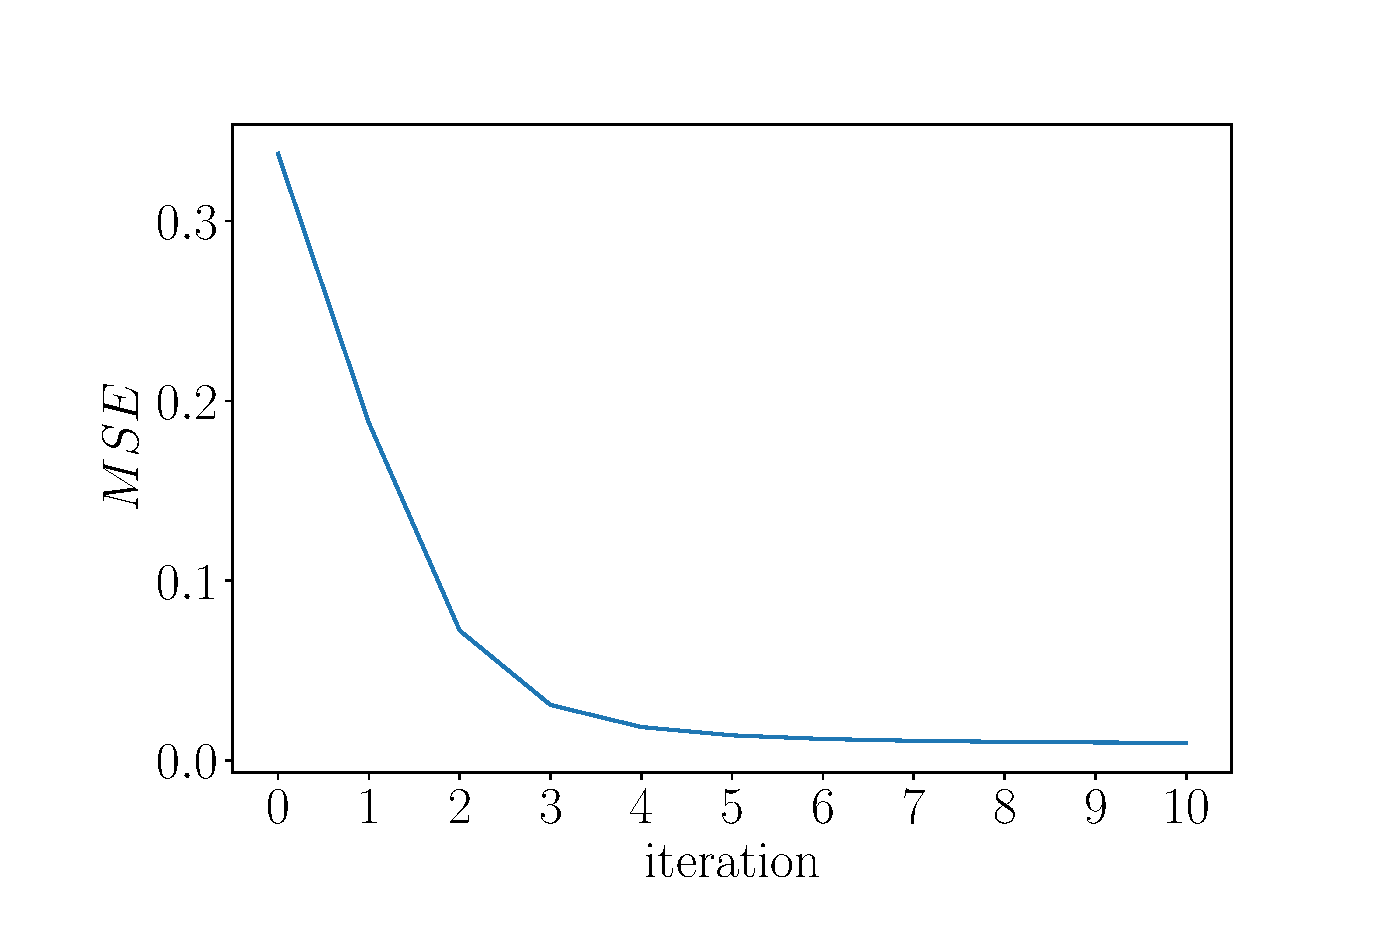
\includegraphics[width=0.5\textwidth,trim={0 0.5cm 2cm 1cm},clip]{./fig/photos/auto_mse_realworld.eps}
		\caption{\ac{MSE} of the \ac{MLEM} method applied to the pre-recorded data from real-world experiments.}
    \label{e1:mse}
\end{figure}
}% %%}



\begin{figure}[!htb]% %%{
  \centering
  \subfloat[estimate of ionizing radiation intensity $\bm{\lambda}$ (rescaled)] {
    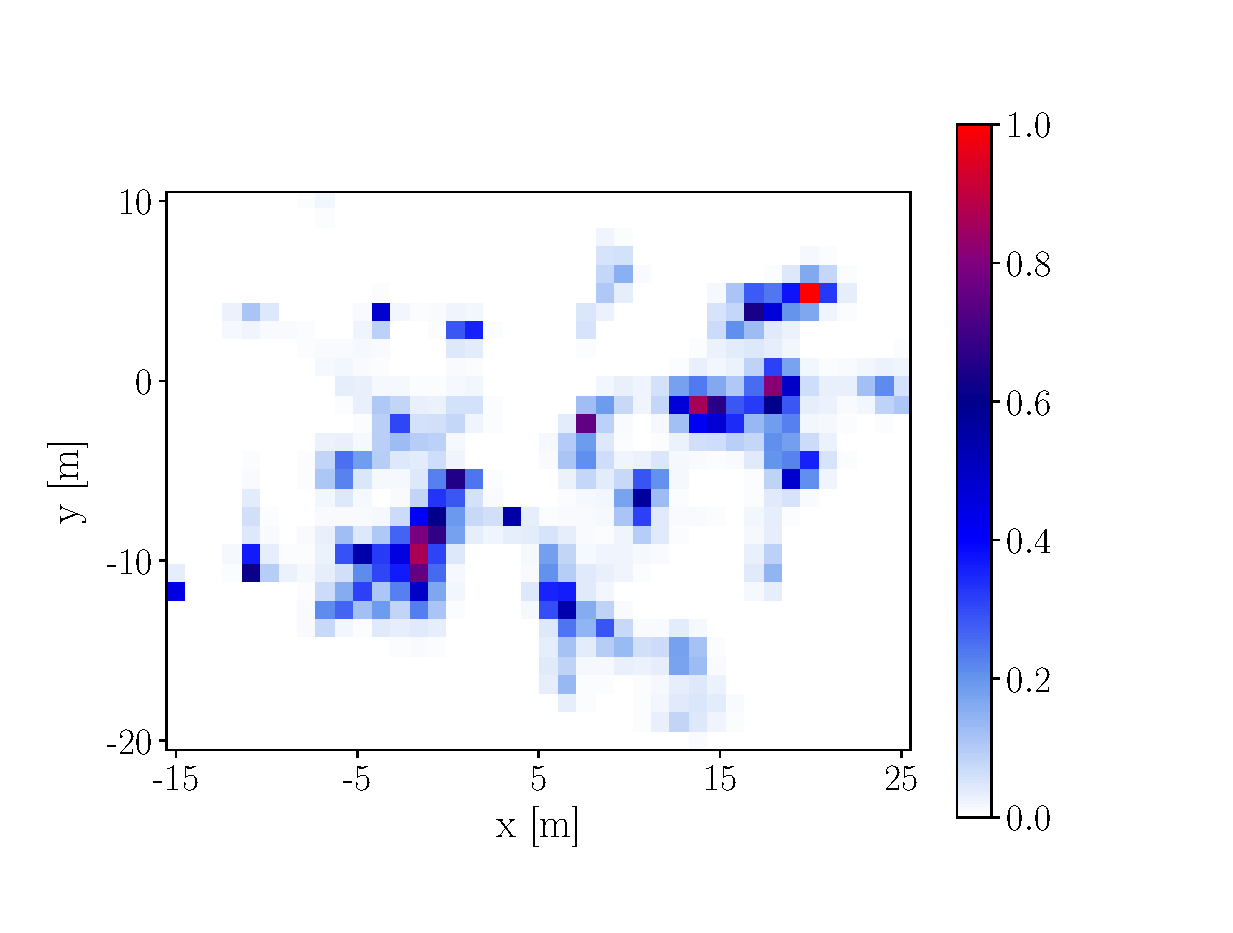
\includegraphics[width=0.5\textwidth,trim={0 0.5cm 2cm 1cm},clip]{./fig/photos/auto_lam.eps}
    \label{e1:lam}
  }
  \subfloat[ground truth positions of sources ($\si{\mega\becquerel}$)] {
    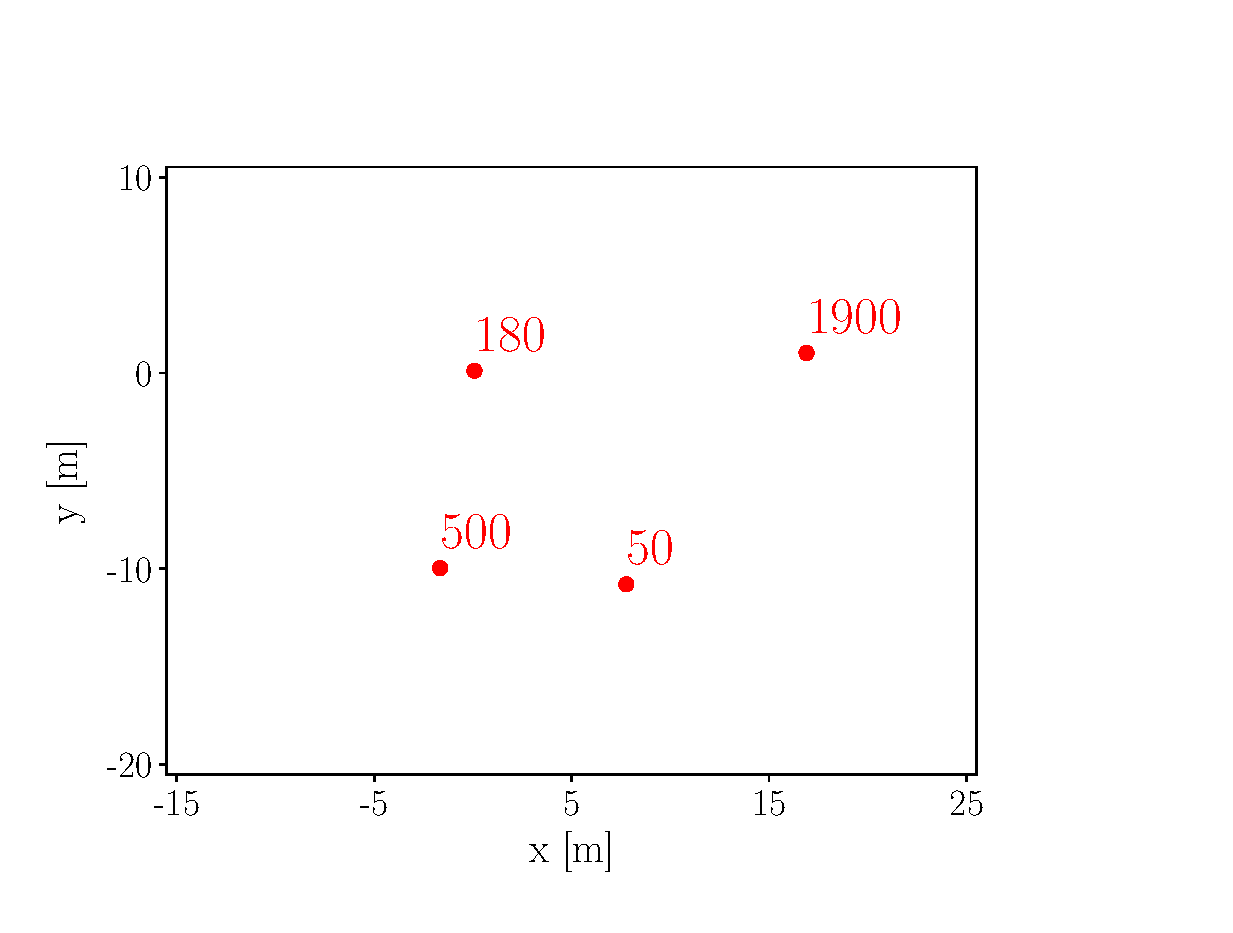
\includegraphics[width=0.5\textwidth,trim={0 0.5cm 2cm 1cm},clip]{./fig/photos/auto_gt.eps}
    \label{e1:gt}
  }
  \newline
  \noindent 
  \subfloat[back-projection (number of Compton cones)] {
    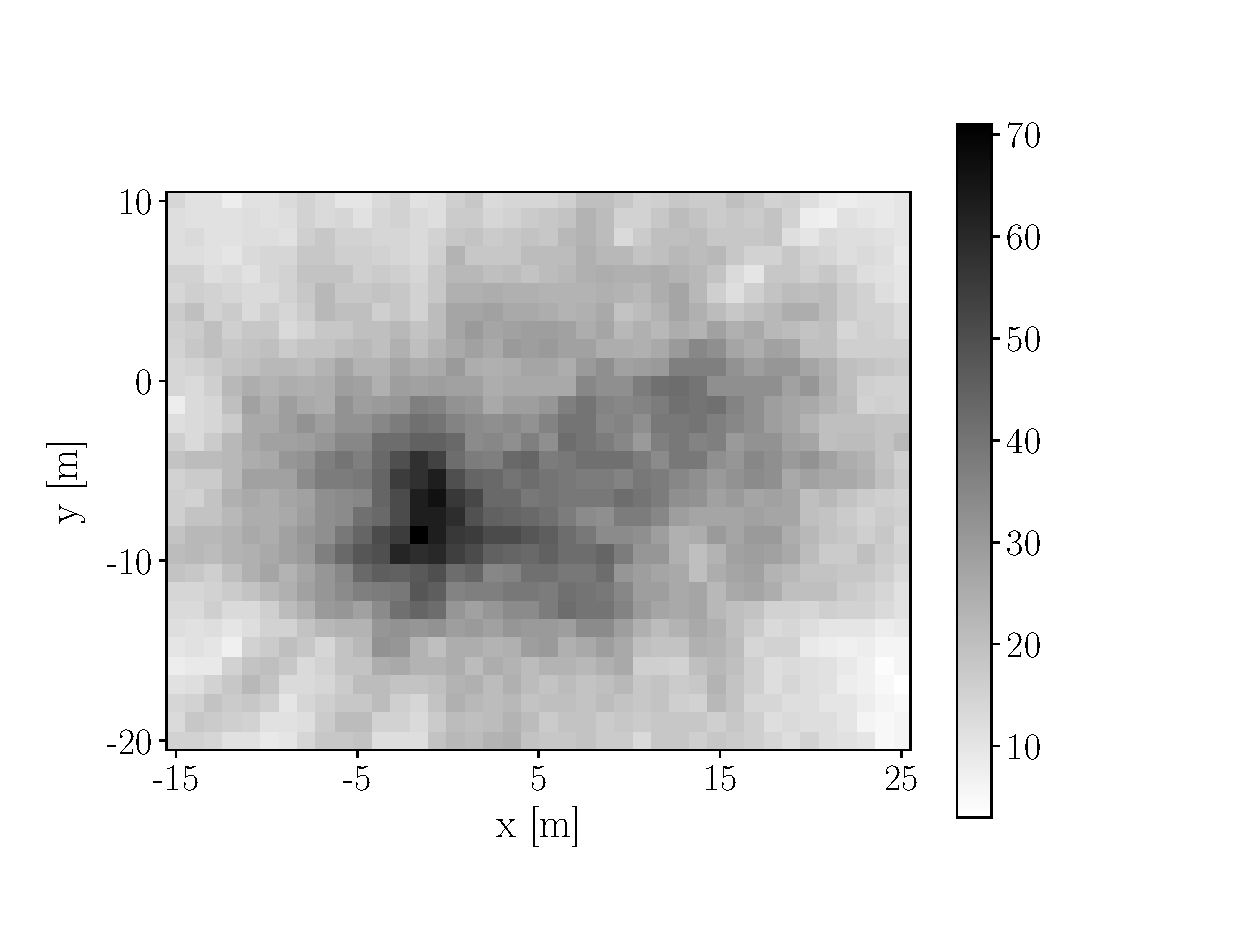
\includegraphics[width=0.5\textwidth,trim={0 0.5cm 2cm 1cm},clip]{./fig/photos/auto_bp.eps}
    \label{e1:bp}
  }
  \subfloat[sensitivity of detection $\mathbf{s}$] {
    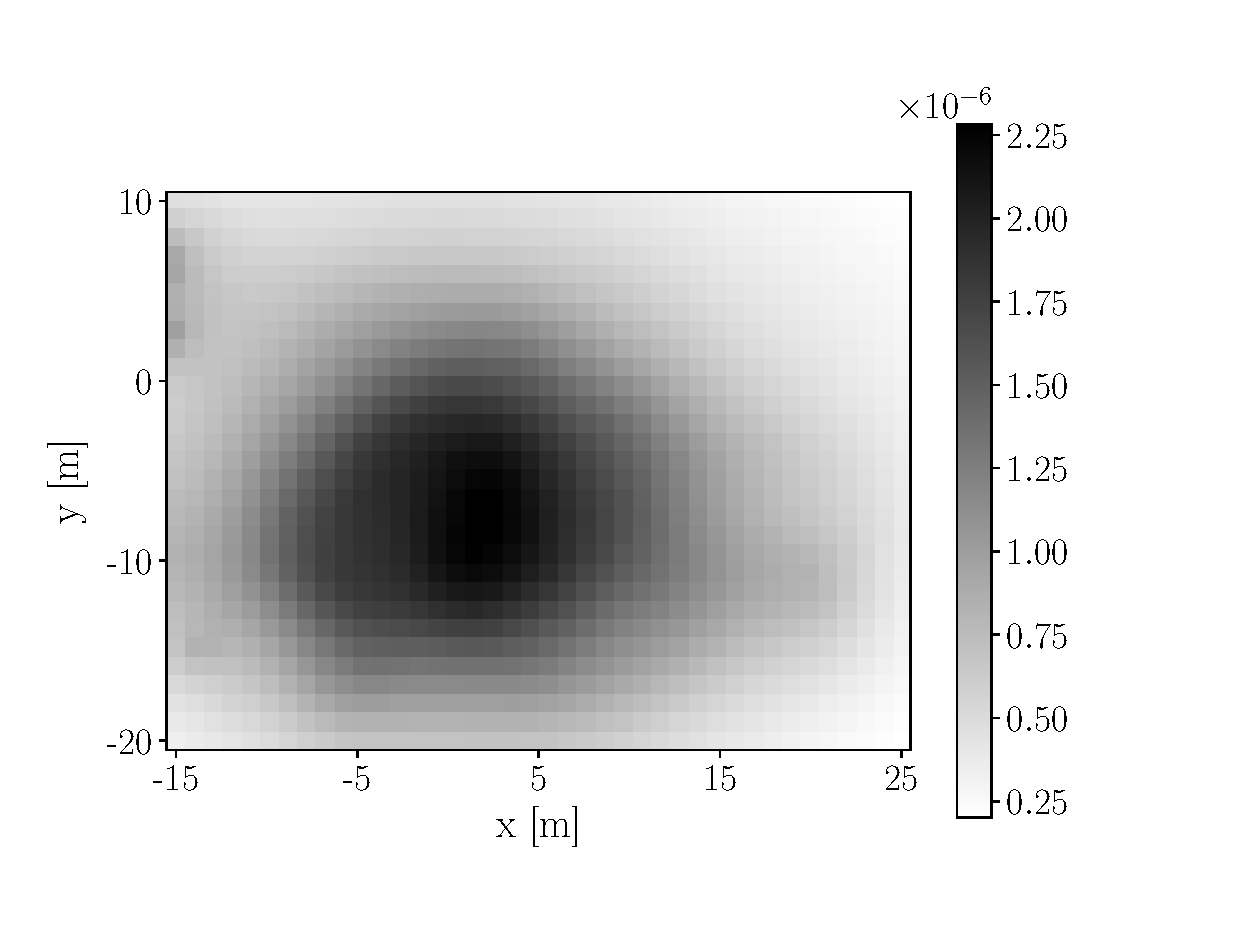
\includegraphics[width=0.5\textwidth,trim={0 0.5cm 2cm 1cm},clip]{./fig/photos/auto_sen.eps}
    \label{e1:sen}
  }
  \caption{The \ac{MLEM} method evaluated on pre-recorded real-world data.}
  \label{fig:e1_all}
\end{figure}% %%}
%%%%%%%%%%%%%%%%%%%%%%%%%%%
\subsection{Summary}
The results of the \ac{MLEM} reconstruction are heavily affected by a noise in measurements.
First of all, the \ac{UAV}s were localized using \ac{GPS} method that might be effected by a position error of several meters.
The position error propagates to the uncertainty of the Compton cone origins.
Furthermore, the real \ac{pix} sensors produced many outliers --- e.g. Compton cones pointing upwards or not intersecting any source position. 
The noisy measurements are probably caused by the working principle of an unshielded single-layer Compton camera, where ionizing particles coming from different directions might affect the Cone reconstruction procedure.
This might be a limiting factor for the localization of multiple sources of ionizing radiation (with high emission activity) that are close to each other.
The single-layer Compton camera is able to estimate the direction of incoming ionizing photons only if the number of interactions detected by the Timepix3 pixel detector inside the \ac{pix} sensor is relatively low and corresponding interactions can be paired together correctly.
However, the presence of multiple sources in close vicinity increases the particle flux and may potentially increase the number of outliers.

In summary, the comparison of \ac{MLEM} estimate (\autoref{e1:lam}) and back-projection (\autoref{e1:bp}) show that the \ac{MLEM} significantly improved the reconstruction quality.
The $\SI{1900}{\mega\becquerel}$ source was localized (despite the low number of recorded photons originating there) 
thanks to the weighting of the estimate with the sensitivity of detection in the \ac{MLEM} algorithm.
Better results might be achieved by using an active search strategy, where the drones are controlled in order to improve the quality of the current \ac{MLEM} estimate.









%%%%%%%%%%%%%%%%%%%%%%%%%%%%%%%%%%%%%%%%%%%%%%%%%%%%%%%%
%%%%%%%%%%%%%%%%%%%%%%%%%%%%%%%%%%%%%%%%%%%%%%%%%%%%%%%%%%%%%%%%%%%%%
%%%%%%%%%%%%%%%%%%%%%%%%%%%%%%%%%%%%%%%%%%%%%%%%%%%%%%%%%%%%%%

\section{Evaluation of MLEM and search strategy in simulation\label{chap:exp2}}
The \ac{MLEM} estimation method has been tested together with the proposed search strategy in \textit{Gazebo} simulator. 
The results were compared with the back-projection method, that served as a baseline.

\begin{figure}[!htb]
  \centering
    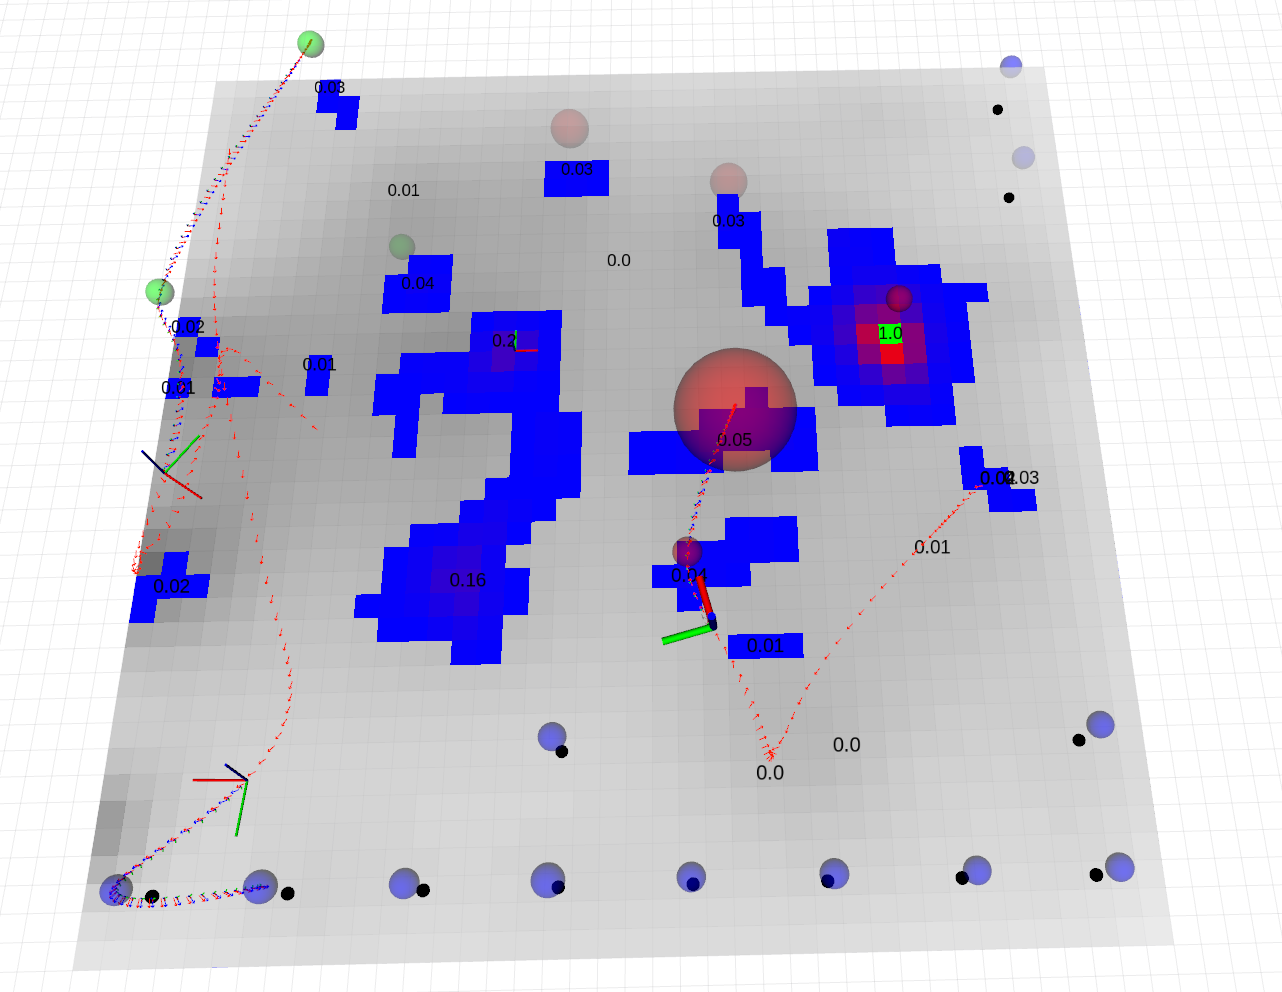
\includegraphics[width=0.9\textwidth]{./fig/photos/simu_search.png}
  \caption{Experiments in \textit{Gazebo} simulator. The \ac{UAV}s are autonomously mapping sources of ionizing radiation place in the area $40 \times 40\ \si{\meter}$ (resolution $r = \SI{1}{\meter}$). 
  The current \ac{MLEM} estimate is visualized using blue-red-green distribution and black numbers denoting the relative activity of local maxima at the given position. 
  The drones follow the trajectories (red arrows) to visit waypoints (depicted as transparent spheres). Two drones are designated for exploitation (red and green waypoints) and one for exploration (blue waypoints).}
  \label{fig:simu_search}
\end{figure}
\subsection{Simulated experiment 1}
%\subsubsection{Experiment setup}
The distribution and activity of the radioactive sources were the same as in the real-world experiments described in the previous section.
Three drones flying $\SI{3}{\meter}$ above the ground were used during the experiment.  
The simulation process (visualized in \textit{RViz}) is shown in \autoref{fig:simu_search}.
Two drones were designated for exploitation (visiting the positions where the sources of radiation are present based on the latest \ac{MLEM} estimate), and one for exploration (visiting positions with the lowest sensitivity). 
The drones were initialized at positions ($-15, -10$), ($-5, -10$) and ($5, -10$) and controlled by the proposed search strategy in the rest of the experiment.
\subsubsection{Measurement noise}
Extra noise was added to the measurements to model the real-world conditions.
The inaccuracy in the drone position (resulting in the shifted origin of the Compton cone) was modelled with the Normal distribution $\mathcal{N}(\mu_{pos}, \sigma_{pos})$ with zero means $\mu_{pos} = 0$ and standard deviation $\sigma_{pos} = \SI{1.5}{\meter}$. 
The noise in energy measurements of the simulated \ac{pix} sensor was modeled the Normal distribution $\mathcal{N}(\mu_{energy}, \sigma_{energy})$ with zero mean $\mu_{energy} = 0$ and standard deviation $\sigma_{energy} = \SI{7}{\kilo\electronvolt}$.

\subsubsection{Results}
The results of the \ac{MLEM} reconstruction are presented in \autoref{fig:e2}.
The progress of radiation mapping is illustrated in \autoref{e2:lam1} (time $t = \SI{25}{\second}$) and \autoref{e2:lam2} ($t = \SI{100}{\second}$), corresponding sensitivity of detection is presented in \autoref{e2:sen1}, \autoref{e2:sen2}.
The active search strategy controlled the drones in order to acquire more measurements, which significantly improved the initial inaccurate estimate (based on a smaller number of Compton cones).
We may notice that after $\SI{100}{\second}$ of flight the \ac{UAV}s correctly localized the $\SI{1900}{\mega\becquerel}$ , $\SI{500}{\mega\becquerel}$ and $\SI{280}{\mega\becquerel}$ sources of simulated ionizing radiation.
The $\SI{50}{\mega\becquerel}$ source was not recognized due to its low emission activity or because it was filtered out during the later iterations of the \ac{MLEM} algorithm.
The \ac{MLEM} method significantly improved the solution compared to the back-projection illustrated in \autoref{e2:bp}.

\subsubsection{Summary}
Three sources with the highest emission activity were correctly localized in less than $\SI{100}{\second}$.
The proposed \ac{MLEM} estimation method, together with the autonomous search strategy, worked as intended.
Although the \ac{MLEM} method does not estimate the positions of sources perfectly for a small number of measurements, the active search strategy guides the \ac{UAV}s in order to acquire more measurements, which further improves the estimate's quality.
The extensive testing in simulations showed that the inaccuracy in the Compton cones' origins significantly reduces the quality of reconstruction, which highlights the need for accurate localization of drones during real-world experiments.
In summary, the experiment showed that the proposed method is capable of autonomous localization of multiple sources of ionizing radiation (of different emission activity).




\subsubsection{Simulation vs. reality}
The simulated noise in the drone's position and energies helped to bring the simulation closer to real-world conditions.
However, the used simulator of ionizing radiation simulates each source-sensor pair independently, which ignores the fact that ionizing particles from multiple sources might interact in the sensor at the same time (causing outliers), therefore the simulation is not as accurate as it could be.
Improving the simulator in order to process interactions caused by different sources simultaneously presents a possible direction for future research.

\begin{figure}[!htb]% %%{
  \centering
  \subfloat[($t = \SI{25}{\second}$) source intensities $\bm{\lambda}$ (rescaled) ] {
    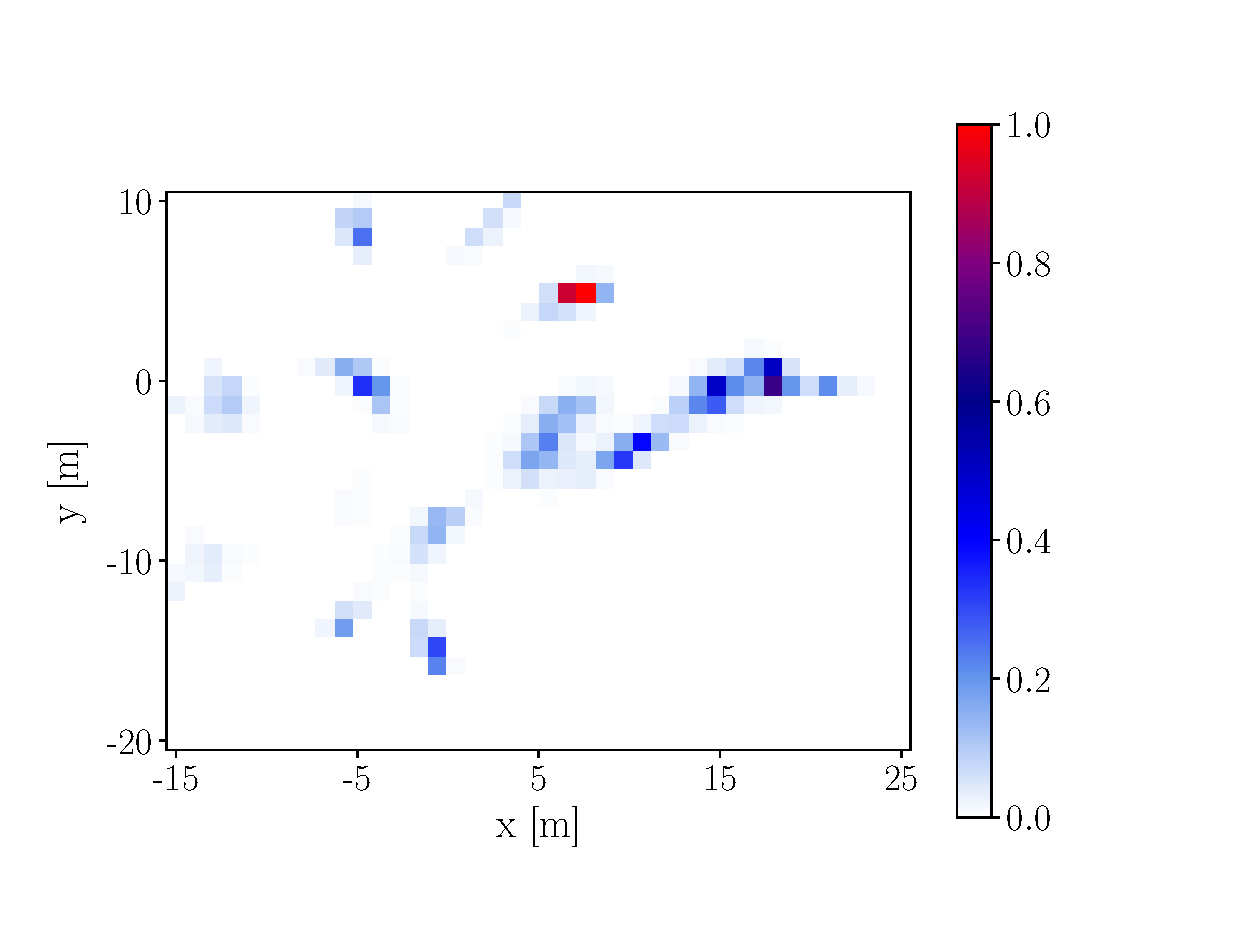
\includegraphics[width=0.5\textwidth,trim={0 0.5cm 2cm 1cm},clip]{./fig/photos/auto_simulation_lam_1.eps}
    \label{e2:lam1}
  }
  \subfloat[($t = \SI{25}{\second}$) sensitivity of detection $\mathbf{s}$ ] {
    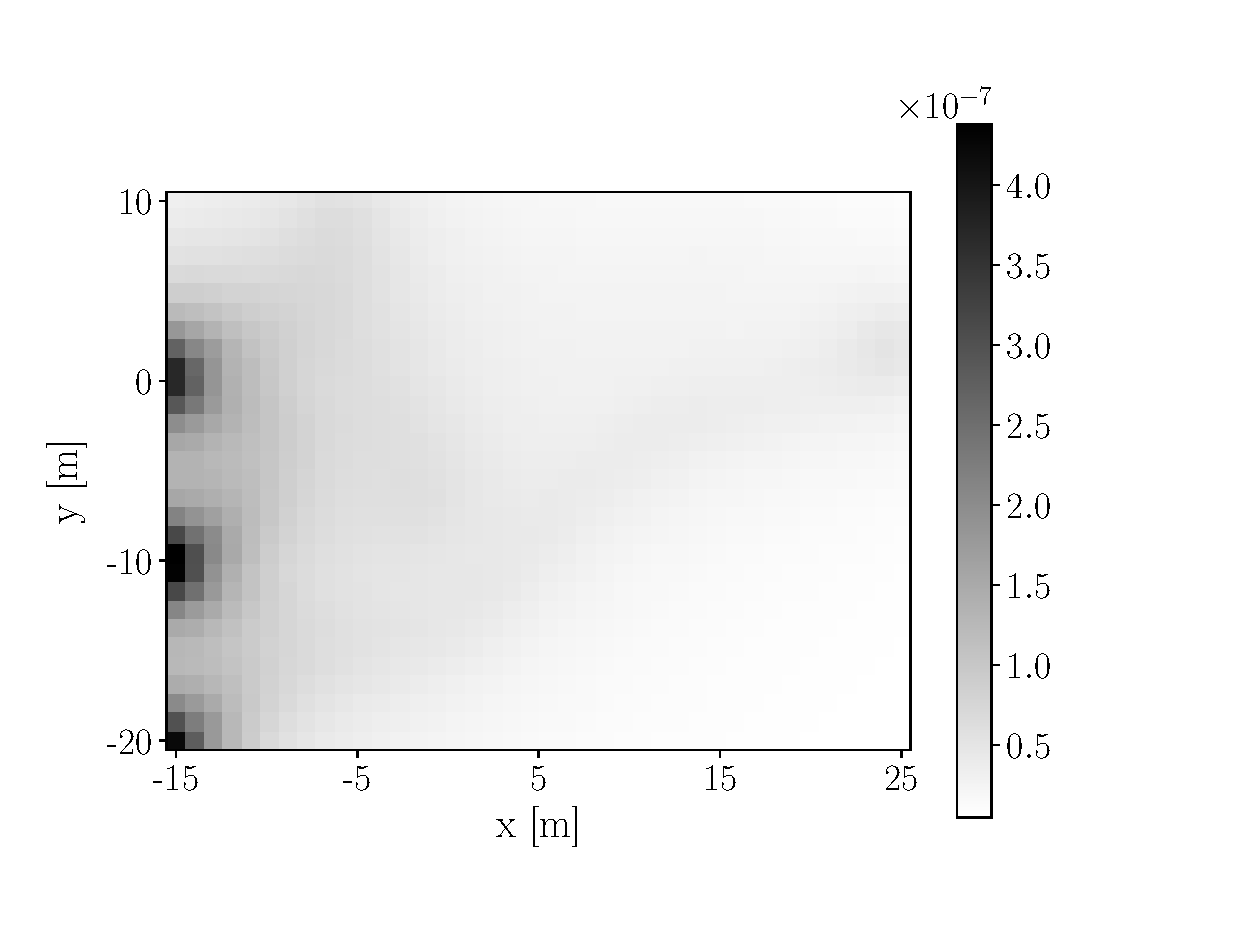
\includegraphics[width=0.5\textwidth,trim={0 0.5cm 2cm 1cm},clip]{./fig/photos/auto_simulation_sen_1.eps}
    \label{e2:sen1}
  }
  \newline
  \noindent
  \subfloat[($t = \SI{100}{\second}$) source intensities $\bm{\lambda}$ (rescaled) ] {
    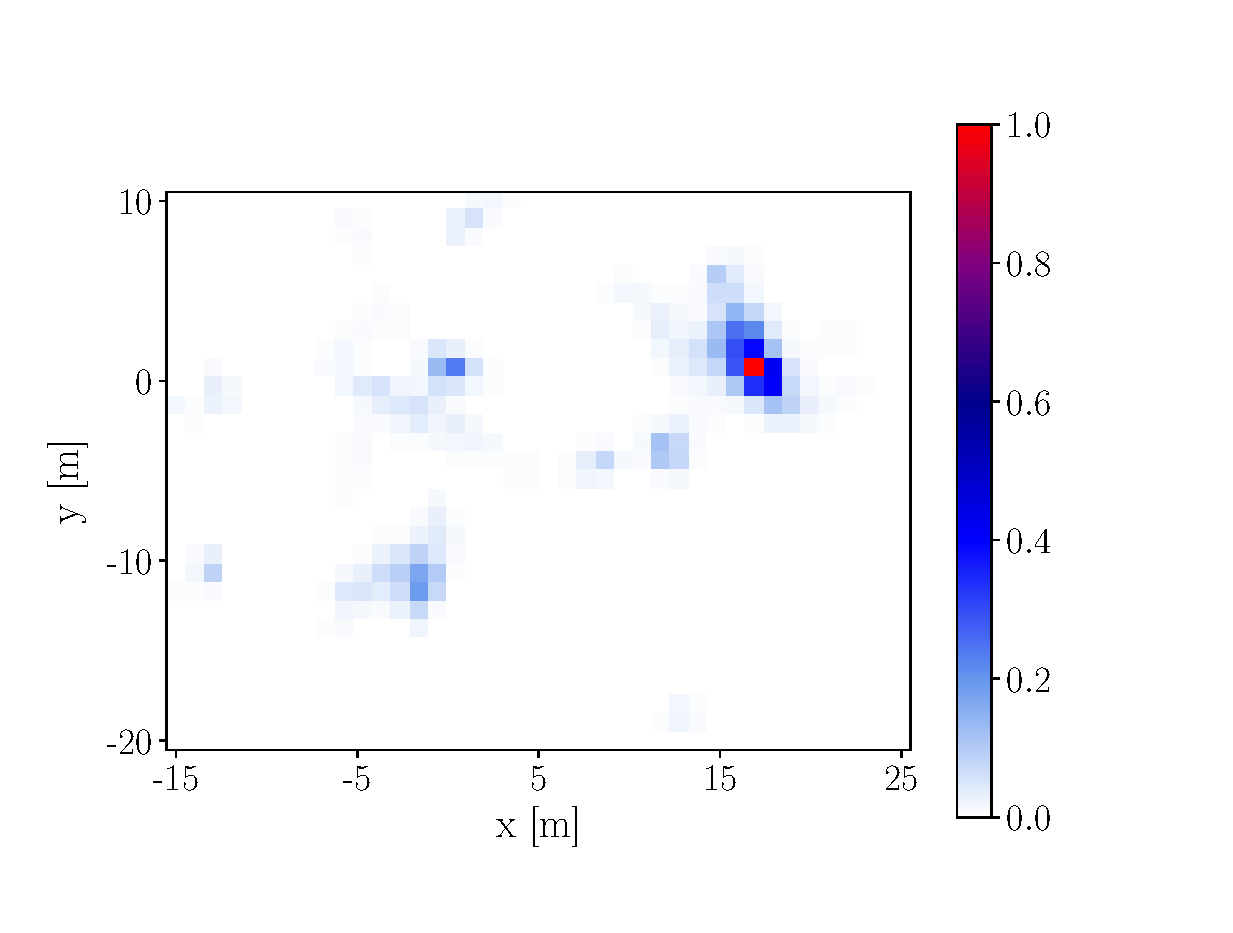
\includegraphics[width=0.5\textwidth,trim={0 0.5cm 2cm 1cm},clip]{./fig/photos/auto_simulation_lam_2.eps}
    \label{e2:lam2}
  }
  \subfloat[($t = \SI{100}{\second}$) sensitivity of detection $\mathbf{s}$ ] {
    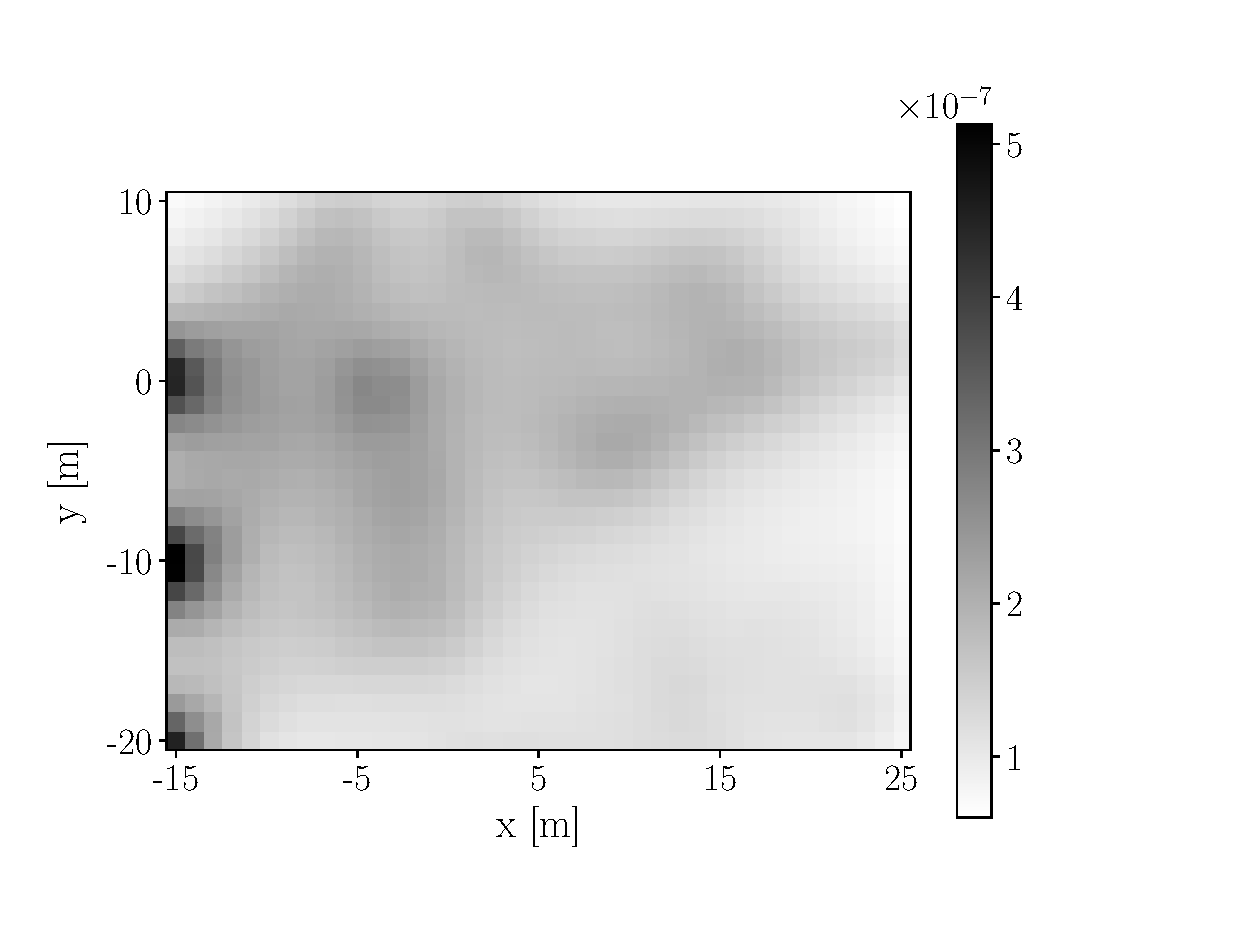
\includegraphics[width=0.5\textwidth,trim={0 0.5cm 2cm 1cm},clip]{./fig/photos/auto_simulation_sen_2.eps}
    \label{e2:sen2}
  }
  \newline
  \noindent
  \subfloat[($t = \SI{100}{\second}$) back projection (number of cones)] {
    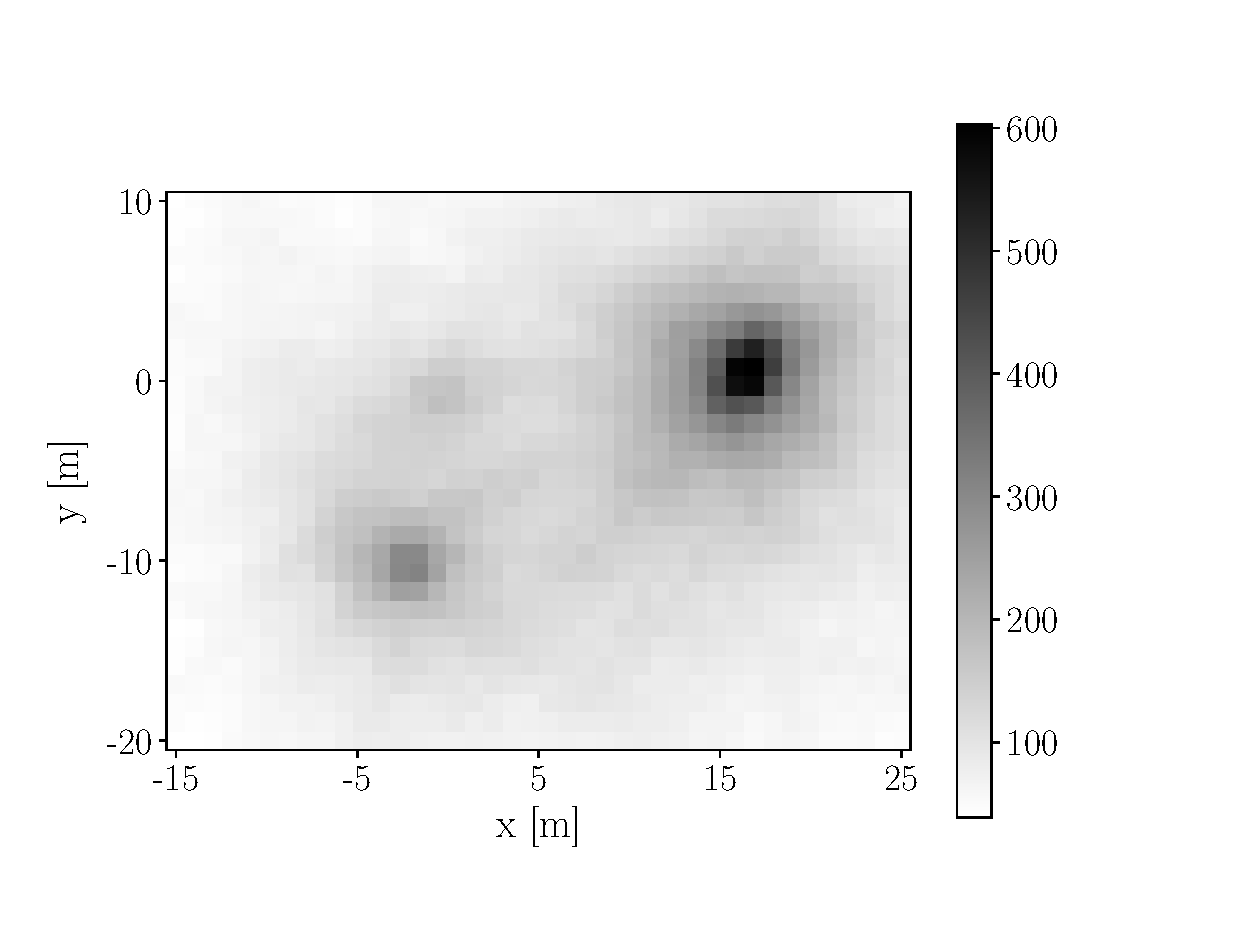
\includegraphics[width=0.5\textwidth,trim={0 0.5cm 2cm 1cm},clip]{./fig/photos/auto_simulation_bp.eps}
    \label{e2:bp}
  }
  \subfloat[ground truth positions of sources ($\si{\mega\becquerel}$)] {
    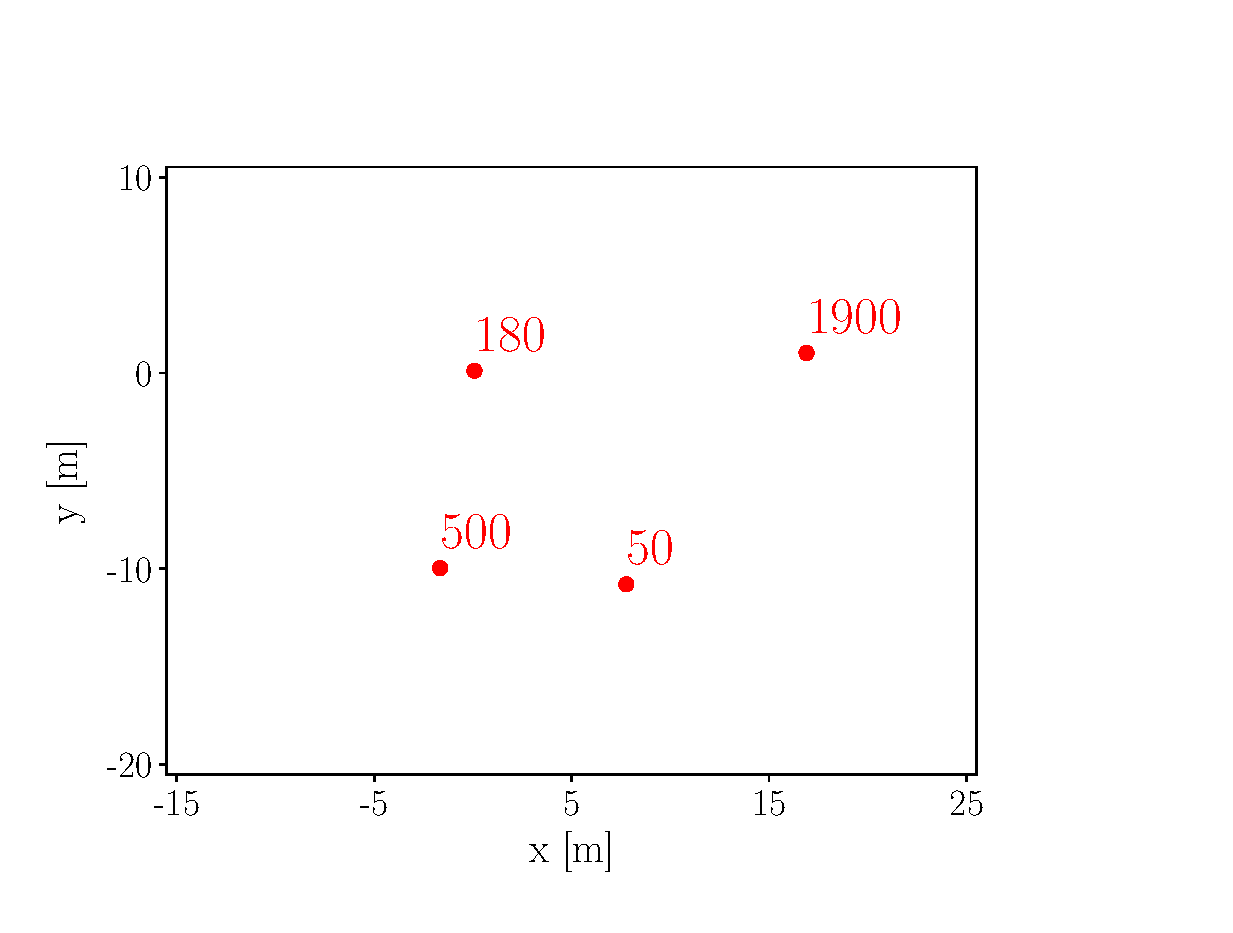
\includegraphics[width=0.5\textwidth,trim={0 0.5cm 2cm 1cm},clip]{./fig/photos/auto_simulation_gt.eps}
    \label{e2:gt}
  }
  \caption{Results of the experiment with three \ac{UAV}s and four sources of ionizing radiation simulated in \textit{Gazebo}. 
  The progress of the \ac{MLEM} reconstruction method is shown in \protect\subref{e2:lam1}, \protect\subref{e2:sen1} and \protect\subref{e2:lam2}, \protect\subref{e2:sen2}.
  %The output of the \ac{MLEM} method after $\SI{25}{\second}$ (\autoref{e2:lam1}, \autoref{e1:sen1}) and after $\SI{100}{\second}$ (\autoref{e2:lam2}, \autoref{e1:sen2}) is presented. 
  %We can see that the quality of the \ac{MLEM} estimate improved during the flight thanks to the active search strategy.
  The back-projection of all cones measured in the first $\SI{100}{\second}$ is shown in \protect\subref{e2:bp}.  }
  \label{fig:e2}
\end{figure}% %%}


\mycomment{
\begin{figure}[!htb]% %%{
  \centering
  \subfloat[($t = \SI{25}{\second}$) source intensities $\bm{\lambda}$ (rescaled) ] {
    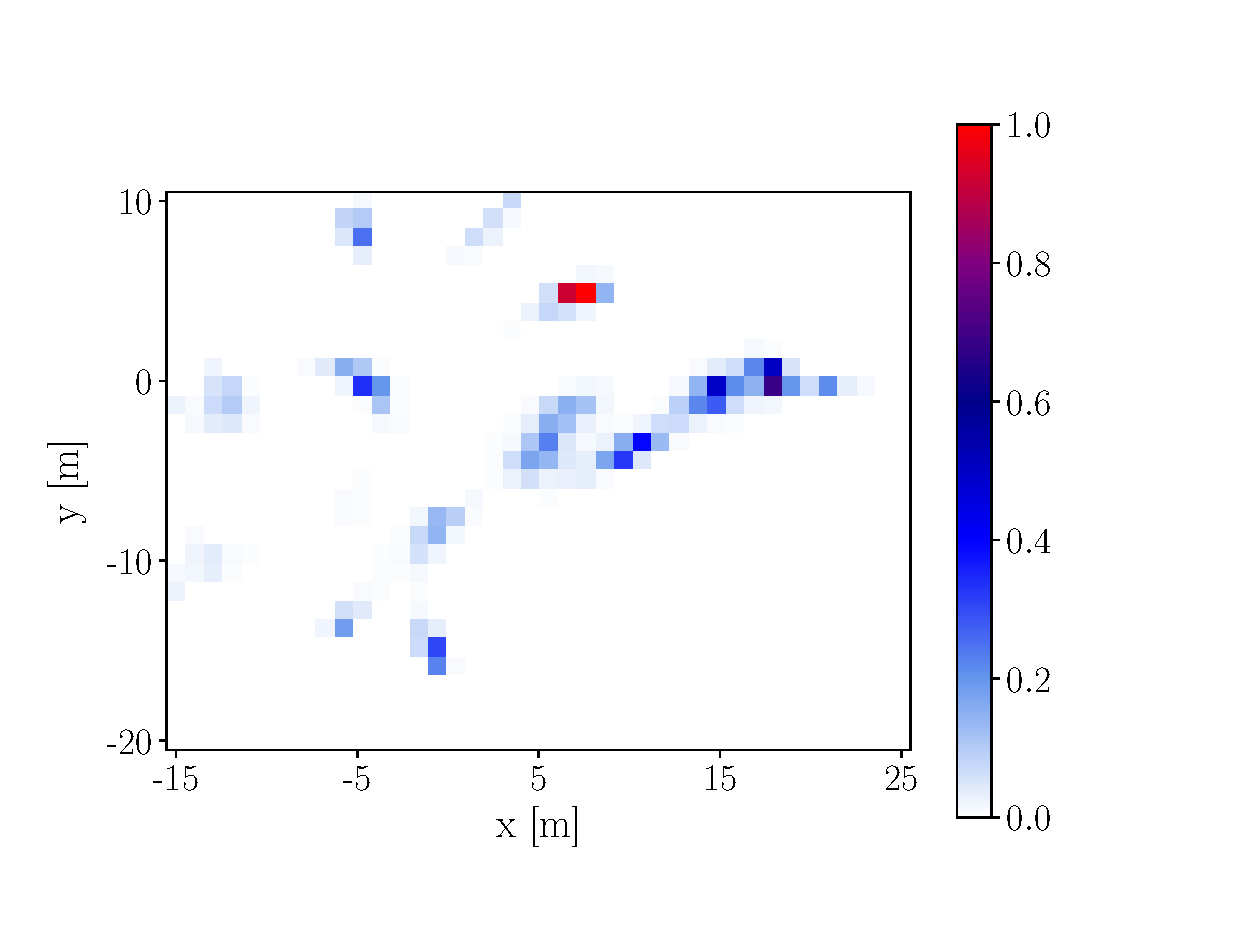
\includegraphics[width=0.5\textwidth,trim={0 0.5cm 2cm 1cm},clip]{./fig/photos/auto_simulation_lam_1.eps}
    \label{e2:lam1}
  }
  \subfloat[($t = \SI{25}{\second}$) sensitivity of detection $\mathbf{s}$ ] {
    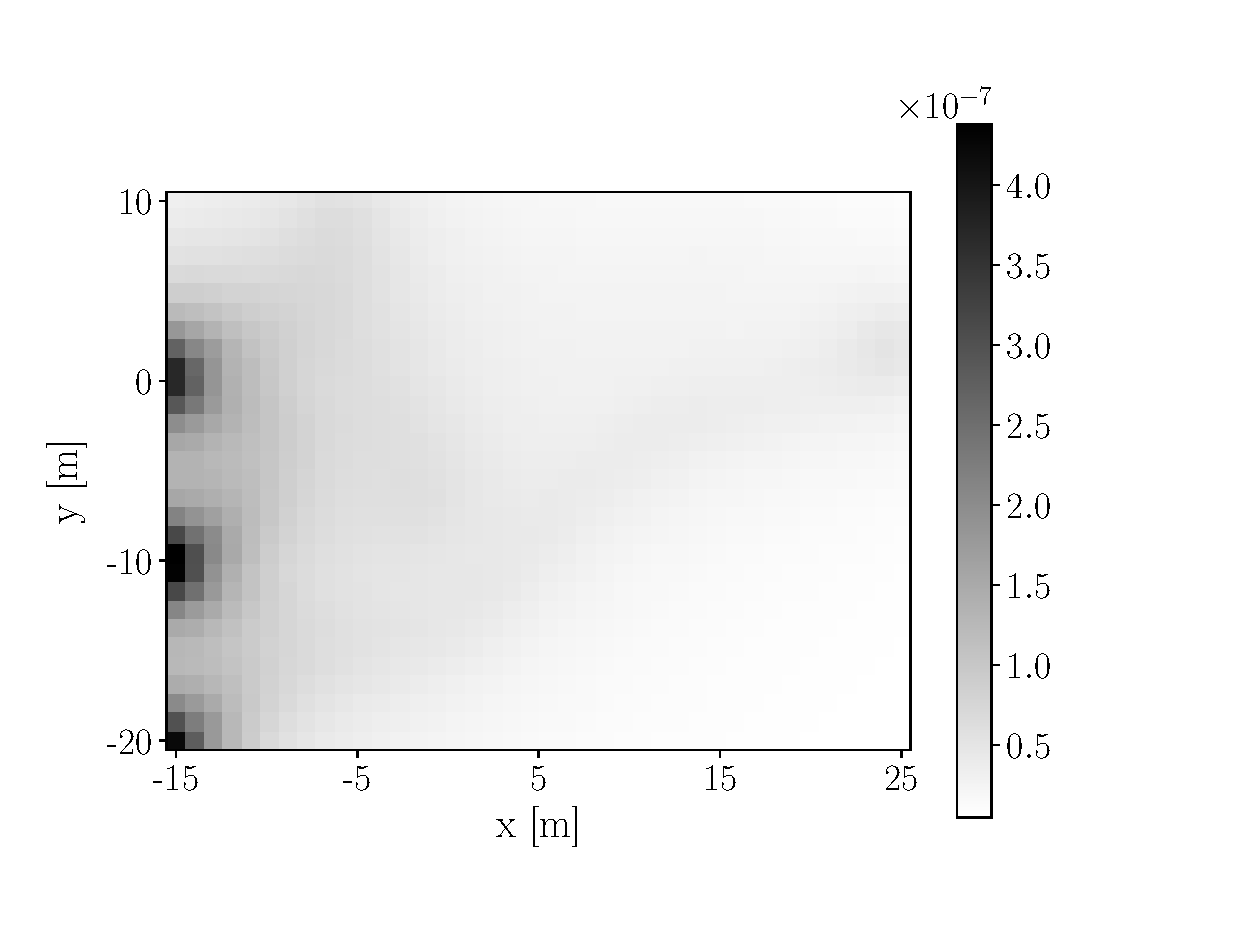
\includegraphics[width=0.5\textwidth,trim={0 0.5cm 2cm 1cm},clip]{./fig/photos/auto_simulation_sen_1.eps}
    \label{e2:sen1}
  }
  \newline
  \noindent
  \subfloat[($t = \SI{100}{\second}$) source intensities $\bm{\lambda}$ (rescaled) ] {
    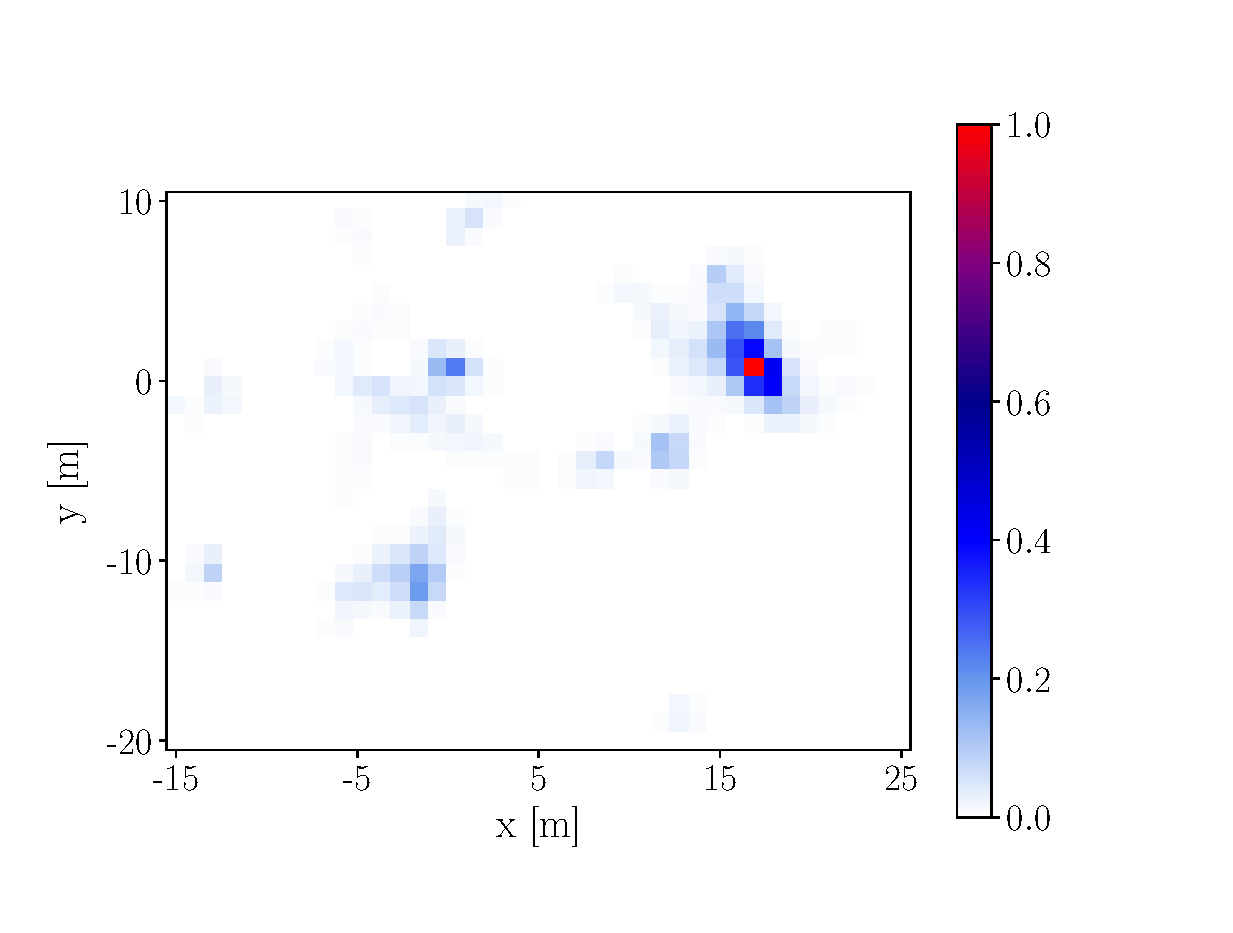
\includegraphics[width=0.5\textwidth,trim={0 0.5cm 2cm 1cm},clip]{./fig/photos/auto_simulation_lam_2.eps}
    \label{e2:lam2}
  }
  \subfloat[($t = \SI{100}{\second}$) sensitivity of detection $\mathbf{s}$ ] {
    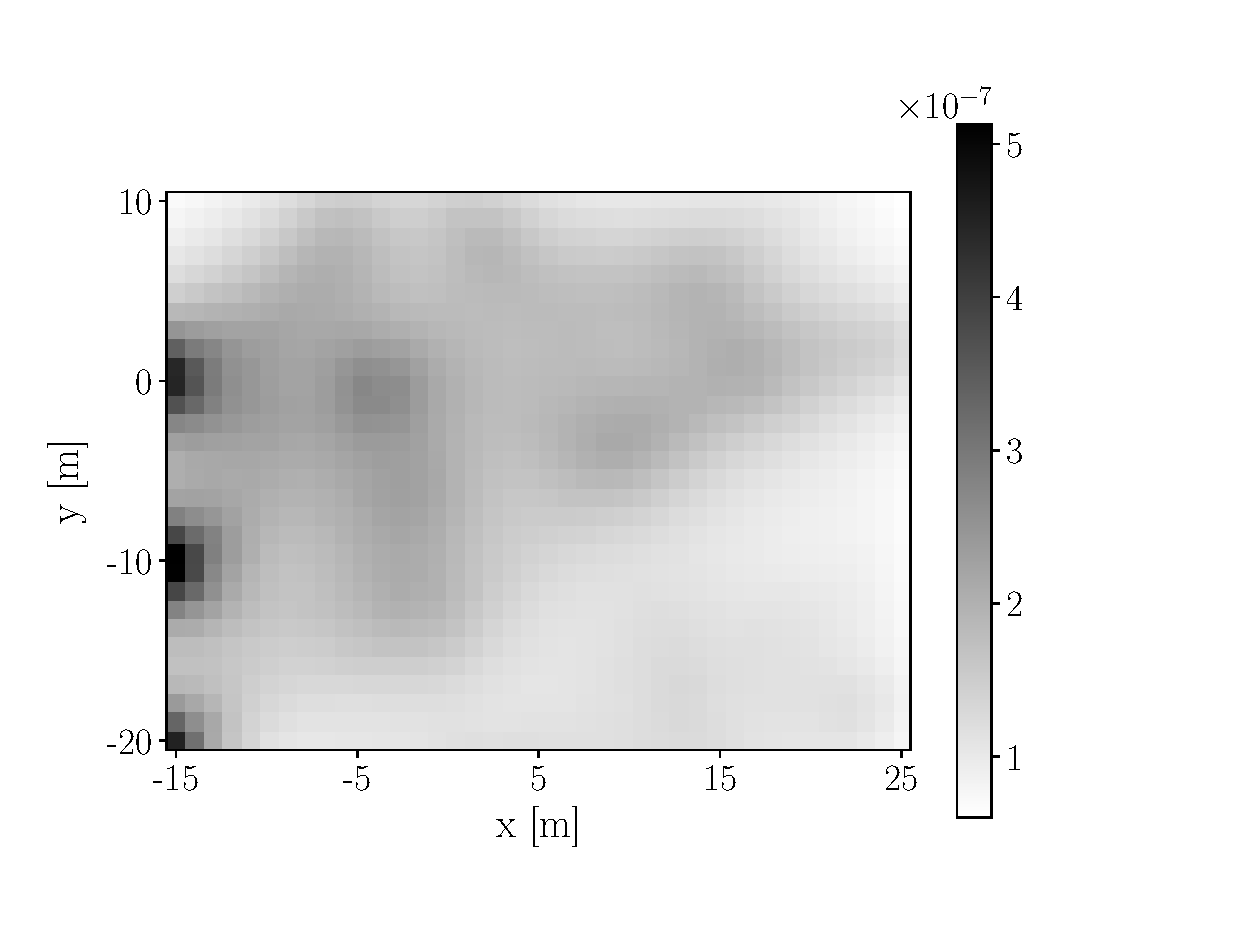
\includegraphics[width=0.5\textwidth,trim={0 0.5cm 2cm 1cm},clip]{./fig/photos/auto_simulation_sen_2.eps}
    \label{e2:sen2}
  }
  \newline
  \noindent
  \subfloat[($t = \SI{100}{\second}$) back projection (number of cones)] {
    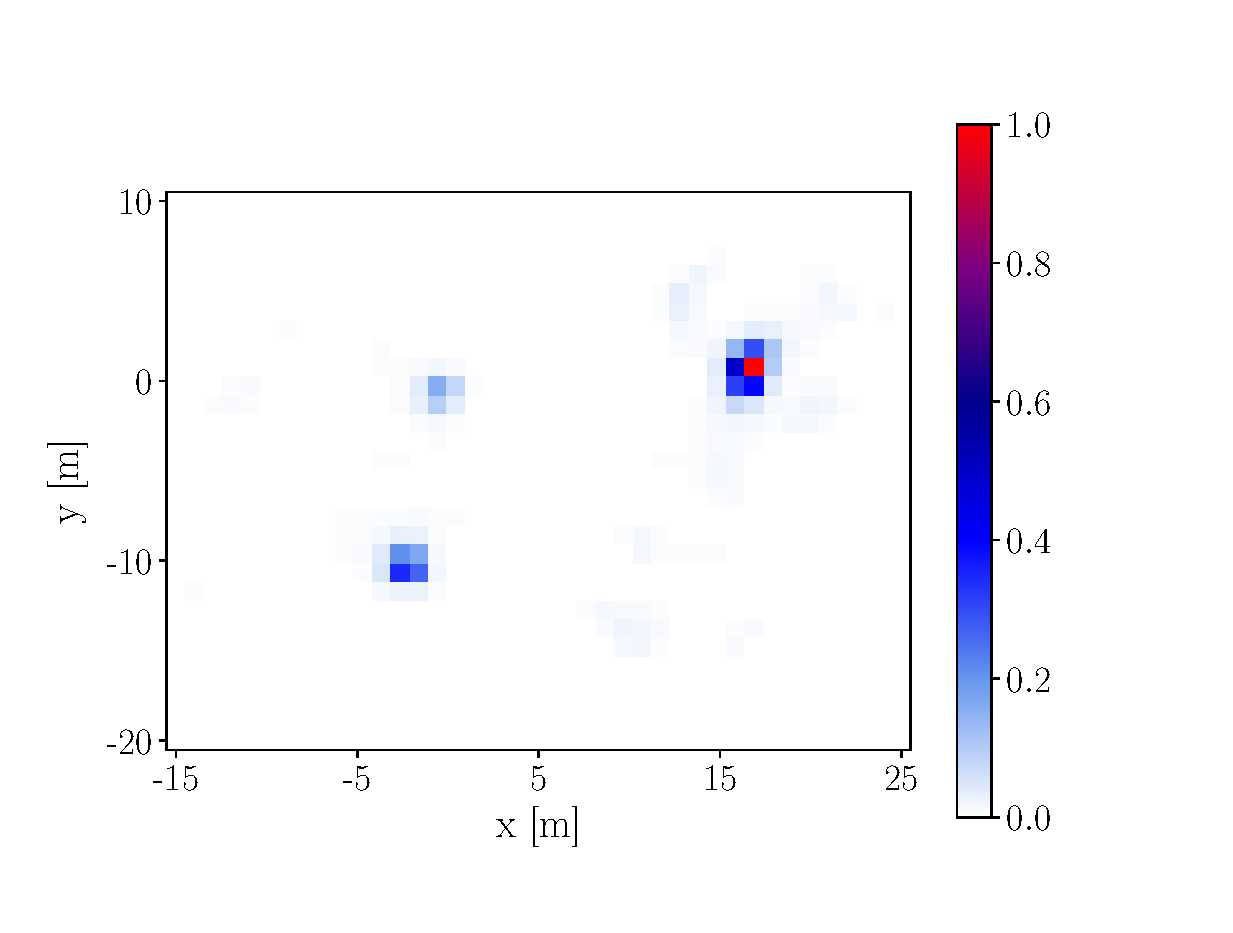
\includegraphics[width=0.5\textwidth,trim={0 0.5cm 2cm 1cm},clip]{./fig/photos/auto_simulation_lam.eps}
    \label{e2:bp}
  }
  \subfloat[ground truth positions of sources ($\si{\mega\becquerel}$)] {
    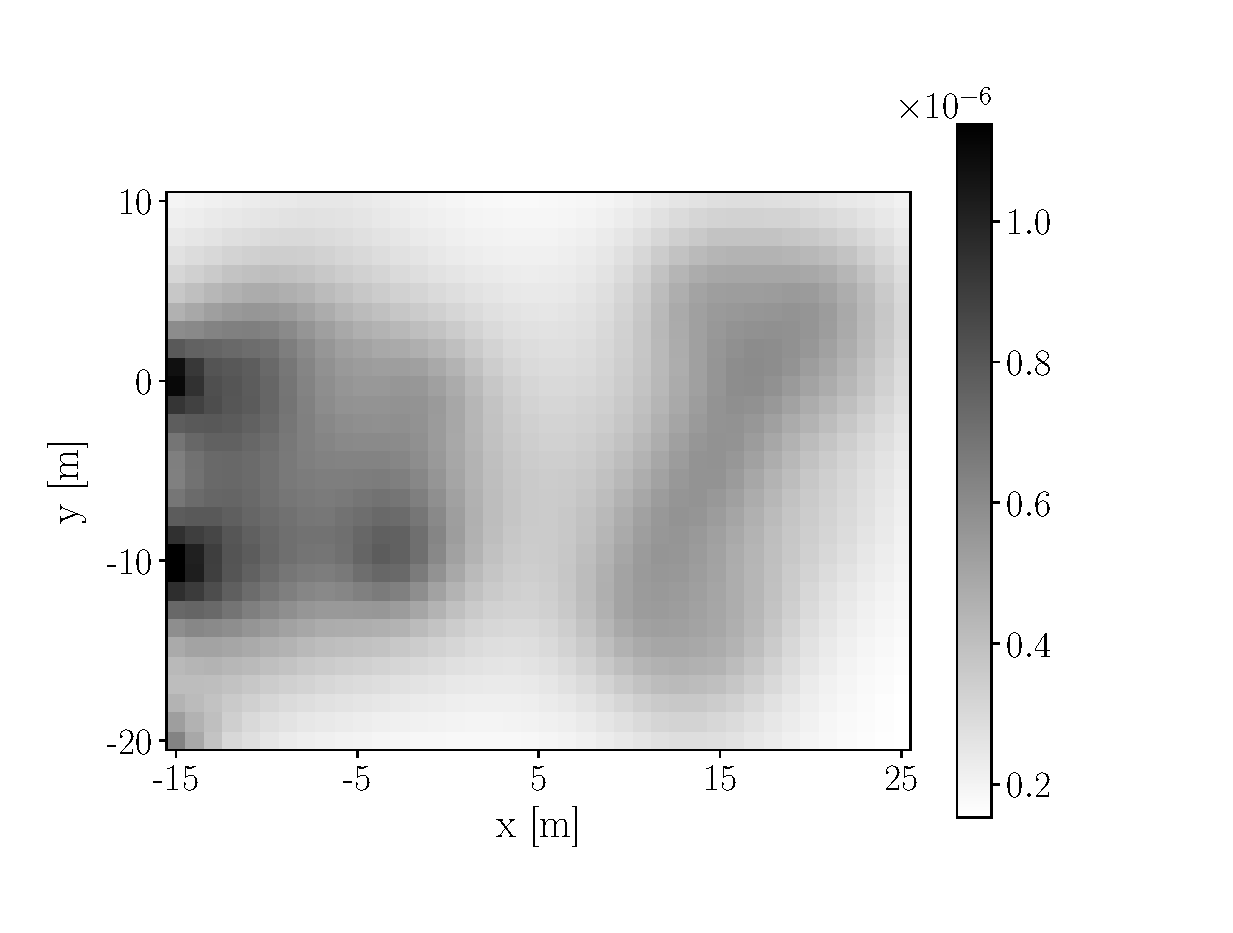
\includegraphics[width=0.5\textwidth,trim={0 0.5cm 2cm 1cm},clip]{./fig/photos/auto_simulation_sen.eps}
    \label{e2:gt}
  }
  \caption{Lorem ipsum}
  \label{fig:e2}
\end{figure}% %%}

}
\subsection{Simulated experiment 2}
The ability to map multiple sources of ionizing radiation is demonstrated on the following simulated scenario:
the size of the area, number of drones, simulated noise and other parameters remain the same as in the previous experiment.
Only the activity of sources is set to the same value for convenience.
The source is considered as detected if the estimated emission activity ($\bm{\lambda}$ rescaled to $0-1$ range) at the ground-truth source position exceeds detection threshold $0.5$ (in the vicinity of $\SI{2}{\meter}$ around the ground-truth position) and remains above threshold $0.3$ during the rest of the experiment.
Since the radiation emission is a stochastic process, the same instance was repeated multiple times.
Results are presented in \autoref{fig:eval}. % shows the detection times for multiple simulated sources if the same activity. 
\begin{figure}[!htb]
  \centering
  \subfloat[Four sources with activity $\SI{100}{\mega\becquerel}$] {
    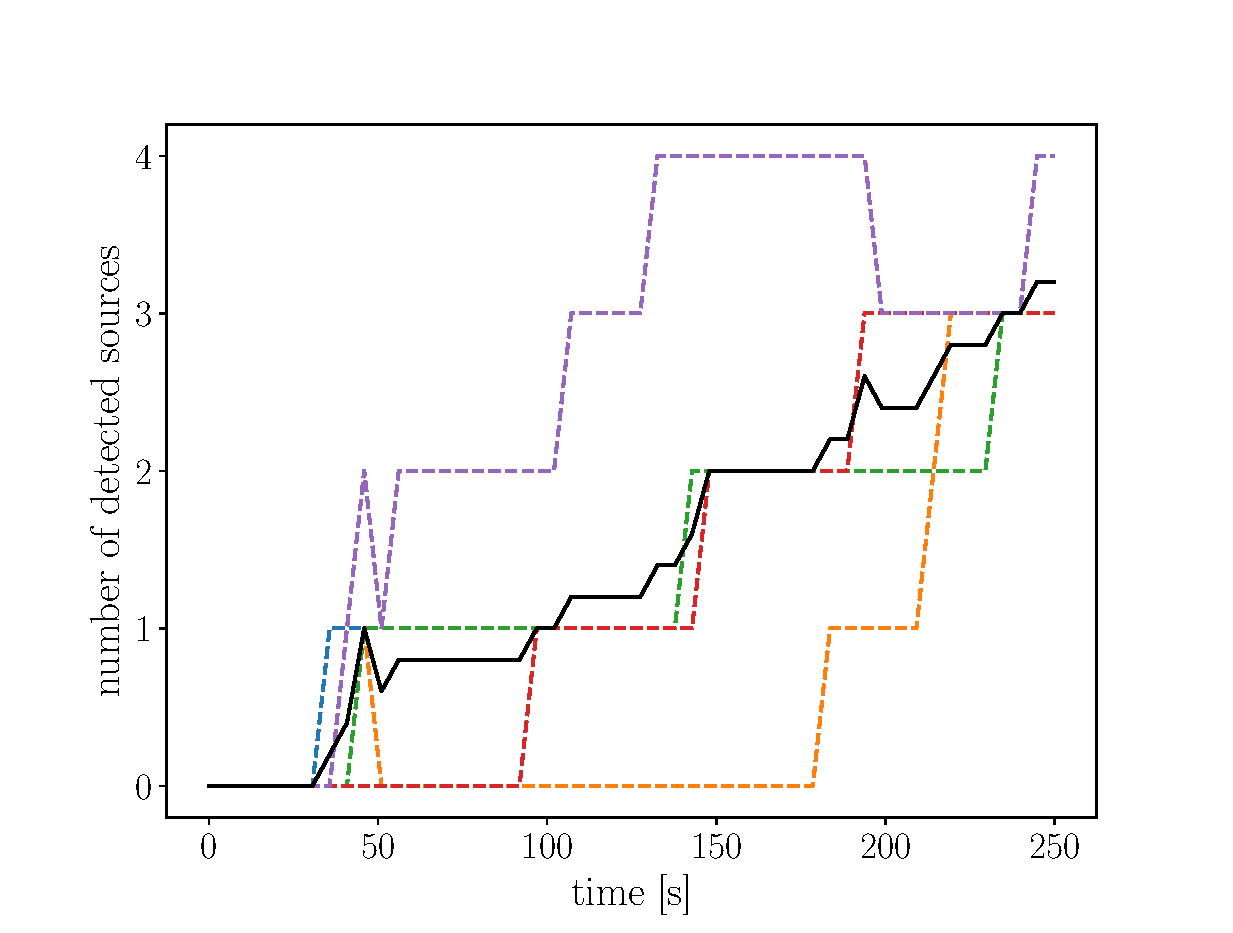
\includegraphics[width=0.4\textwidth,trim={1cm 0 1.5cm 1.2cm},clip]{./fig/photos/auto_eval1.eps}
    \label{fig:eval1}
  }
  \subfloat [Four sources with activity $\SI{500}{\mega\becquerel}$]{
    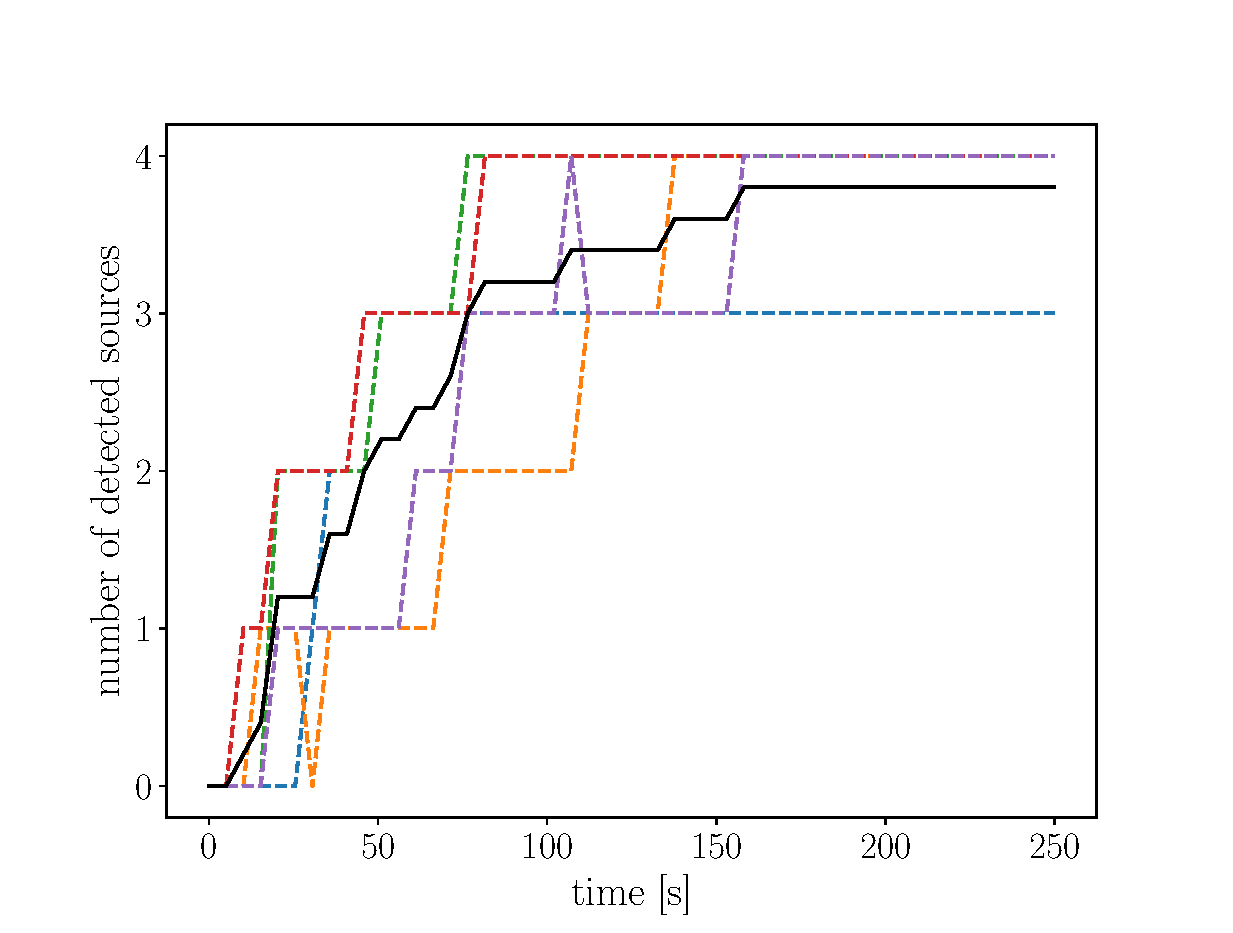
\includegraphics[width=0.4\textwidth,trim={1cm 0 1.5cm 1.2cm},clip]{./fig/photos/auto_eval2.eps}
    \label{fig:eval2}
  }
  \newline\noindent
  \subfloat [Four sources with activity $\SI{2000}{\mega\becquerel}$]{
    \includegraphics[width=0.4\textwidth,trim={1cm 0 1.5cm 1.2cm},clip]{./fig/photos/auto_eval3.eps}
    \label{fig:eval3}
  }
  \subfloat [Ground truth positions]{
    \includegraphics[width=0.45\textwidth,,trim={0cm 0 1.5cm 1.2cm}, clip ]{./fig/photos/auto_eval_gt.eps}
    \label{fig:eval4}
  }
  \caption{The number of correctly detected sources with the same emission activity (located at positions \protect\subref{fig:eval4}). Dashed lines represent the individual experiments (each scenario was repeated $5$ times), the black line is the average. The detection was evaluated every $5$ seconds.}
  \label{fig:eval}
\end{figure}
\subsubsection{Results}
We can see that the low emission activity of the sources prolongs the detection time (\ref{fig:eval1}), however, the method was still able to localize positions of the $3$ sources (on average) in less than $\SI{250}{\second}$.
The method was able to correctly localize four $\SI{2000}{\mega\becquerel}$ sources is less than  $\SI{170}{\second}$ in all scenarios.
We may notice that the number of detected sources also sometimes decreased during the time (see the purple line in \ref{fig:eval3}). 
This shows that the method do not perfectly estimate the relative emission activity of the sources, which is caused by the stochastic nature of radioactive decay and limited number of measurements.



%%%%%%%%%%%%%%%%%%%%%%%%%%%%%%%%%%%%%%%%%%%%%%%%%%%%%%%%%%%%%%%%%%%%%%%
%%%%%%%%%%%%%%%%%%%%%%%%%%%%%%%%%%%%%%%%%%%%%%%%%%%%%%%%%%%%%%%%%%%%%%%%%%
%%%%%%%%%%%%%%%%%%%%%%%%%%%%%%%%%%%%%%%%%%%%%%%%%%%%%%%%%%%%%%%%%%%%%%


\section{Real-world experiment with simulated radiation\label{chap:exp3}}
The proposed search strategy has been tested using real \ac{UAV}s during the field experiments.
Since the real sources of radiation were not available, the ionizing radiation was simulated onboard each \ac{UAV}.
The main purpose of the experiment was to test the search strategy with real hardware and gain some experience with real-world conditions, where many things are not as simple as in simulation.
\begin{figure}[!htb]
  \centering
  \subfloat[The DJI f450 drones used during the experiments.] {
    \includegraphics[width=0.5\textwidth]{./fig/photos/experiments.jpg}
    \label{fig:d1}
  }
  \subfloat [The area of interest and \ac{UAV}s searching for the (simulated) sources of ionizing radiation.]{
    \includegraphics[width=0.5\textwidth]{./fig/photos/pole3.png}
    \label{fig:d2}
  }
  \caption{Field experiments with real hardware. The drones \protect\subref{fig:d1} were mapping the simulated radioactive sources located somewhere in the open field \protect\subref{fig:d2}.}
  \label{fig:field}
\end{figure}
\subsection{Experiment setup}
The size of the explored area was $100 \times 100\ \si{\meter}$, the resolution of each map cell was set to $\SI{0.5}{\meter}$.
The simulator of ionizing radiation was running onboard each \ac{UAV}, simulating the radiation coming from sources at predefined positions.
The \ac{UAV}s were localized using \ac{GPS}.
However, the noise in \ac{GPS} position measurement did not affect the simulated radiation data since the drones used their belief (not the real position) when simulating incoming ionizing photons.
The viewpoints (positions of the drones) were sampled with $\SI{5}{\hertz}$, and the \ac{MLEM} estimate was updated every $\SI{2}{\second}$.
Four simulated sources of $\SI{662}{\kilo\electronvolt}$ photons with activity $2000, 1000, 1000, 500\ \si{\mega\becquerel}$ were located at positions shown in  \autoref{e3:gt}.

%The communication between the base station (notebook with \textit{Intel i5-1240P} processor, $\SI{16}{\giga\byte}$ RAM, $\SI{4}{\giga\byte}$ GPU) and the \ac{UAV}s was established via \ac{wifi} network. 

\subsection{Results}
In the initial phase (from time $t = \SI{0}{\minute}$ to time $t = \SI{2}{\minute}$), the drones flew over the area once in a ``zig-zag'' pattern following the predefined trajectory (covering the area uniformly, as can be seen in \autoref{e3:senzig}) and measured first $17$ Compton cones.
The ``zig-zag'' trajectory was precomputed using the MRS UAV System \cite{mrs_system}.
The \ac{MLEM} estimate and sensitivity of detection after the initial phase is shown in \autoref{e3:lamzig} and \autoref{e3:senzig}.
Then (at the time $t = \SI{2}{\minute}$), the proposed search strategy took control---two drones were designated for exploitation, one for exploration.
The trajectories of the \ac{UAV}s during the search phase (\autoref{e3:paths}) show that the two ``exploitation'' drones focused on acquiring more measurements while the third drone was exploring the unexplored area.
The final estimate of radiation sources intensities (at the end of the experiment $t = \SI{10}{\minute}$) is shown in \autoref{e3:lam}.
Three of four sources of simulated ionizing radiation were correctly localized (together with their relative emission activity, which is shown in table \autoref{tab:temenight_results}).
The weakest $\SI{500}{\mega\becquerel}$ source at position ($75, 75$) was not discovered despite the fact that the exploration drone flew around it multiple times (see blue path in \autoref{e3:paths}).
The minimum distance between the \ac{UAV}s was not below the safety threshold ($\SI{4}{\meter}$) during the whole flight, therefore all the planned trajectories were non-colliding.
267 Compton events were recorded during the whole experiment.
\begin{table}[htb]
\begin{center}
  \begin{tabular}{ |c|c|c|c| } 
 \hline
    \multicolumn{2}{|c}{Sources} &  \multicolumn{2}{|c|}{ relative activity } \\
 \hline
    position & activity & ground truth & MLEM estimate\\ 
 \hline
    (10, 20) & 2000 MBq & 1.0  & \textbf{1.0} \\ 
    (20, 20) & 1000 MBq &  0.5 & \textbf{0.49} \\ 
    (80, 80) & 1000 MBq &  0.5 & \textbf{0.52} \\ 
    (75, 75) & 500 MBq &  0.25 & \textbf{0.0} \\ 
 \hline
\end{tabular}
  \caption{Results of the real-world experiment with simulated data. The last column presents estimated relative activity at the map positions that correspond to the ground truth position of the given source.}
  \label{tab:temenight_results}
\end{center}
\end{table}

\subsection{Summary}
The experiment proved that the whole system be used for fast radiation mapping in large open areas and perform all the computations in real-time.
The proposed search strategy, together with the \ac{MLEM} mapping method, worked as intended.
The initial estimate of source positions was significantly improved during the search phase.
Although the maximum likelihood does not provide an accurate estimate for a small number of cones (see \ac{MLEM} estimate in \autoref{e3:lamzig} generated from 17 Compton cones), the inaccurate estimate ``attracts'' the \ac{UAV}s that come closer and likely measure more ionizing photons, that guide the \ac{UAV}s to the actual position of the source.
This shows that online estimation (together with an active search strategy) is beneficial for the autonomous detection of ionizing radiation.

Three of four sources of simulated radiation were localized during the experiment.
The weakest $\SI{500}{\mega\becquerel}$ was not discovered during the flight, which is probably caused more by the limited sensitivity of the (simulated) \ac{pix} sensor than by the estimation method. It is important to note that the simulated radiation data were generated in ideal conditions, without any noise in the drone position, energies measured in the sensor or particles causing false positive Compton detections.
Therefore the results of \ac{MLEM} reconstruction results are more accurate compared to the previously described experiments with real sources of ionizing radiation.

% Answer: [trim={left bottom right top},clip]
% Ex. 1: trim from left edge
%\includegraphics[width=0.5\textwidth,trim={0 0 2cm 2cm},clip]{./fig/photos/auto_temesvar_drone_paths.eps}


\begin{figure}[ht!]% %%{
  \centering
  
  \subfloat[source intensities $\bm{\lambda}$ after the initial phase ($t = \SI{2}{\minute}$) ] {
    \includegraphics[width=0.5\textwidth,trim={1cm 0 2.5cm 1.2cm},clip]{./fig/photos/auto_temesvar_lamzig.eps}
    \label{e3:lamzig}
  }
  \subfloat[Sensitivity $\mathbf{s}$ after the initial phase ($t = \SI{2}{\minute}$)] {
    \includegraphics[width=0.5\textwidth,trim={1cm 0 2.5cm 1.2cm},clip]{./fig/photos/auto_temesvar_senzig.eps}
    \label{e3:senzig}
  }
  \newline
  \noindent 
  \subfloat[final estimate of source intensities $\bm{\lambda}$($t = \SI{10}{\minute}$)] {
    \includegraphics[width=0.5\textwidth,trim={1cm 0 2.5cm 1.2cm},clip]{./fig/photos/auto_temesvar_lam.eps}
    \label{e3:lam}
  }
  \subfloat[Sensitivity $\mathbf{s}$ at the end of the experiment ($t = \SI{10}{\minute}$)] {
    \includegraphics[width=0.5\textwidth,trim={1cm 0 2.5cm 1.2cm},clip]{./fig/photos/auto_temesvar_sen.eps}
    \label{e3:sen}
  }
  \newline
  \noindent 
  \subfloat[ground truth ($\si{MBq}$)] {
    \includegraphics[width=0.5\textwidth,trim={1cm 0 2.5cm 1.7cm},clip]{./fig/photos/auto_temesvar_gt.eps}
    \label{e3:gt}
  }
  \subfloat[Paths of \ac{UAV}s during the search phase \newline (red, green --- exploitation, blue --- exploration)] {
    \includegraphics[width=0.5\textwidth,trim={1cm 0 2.5cm 1.7cm},clip]{./fig/photos/auto_temesvar_drone_paths.eps}
    \label{e3:paths}
  }
  %\subfloat[Final back-propagation.] {
  %  \includegraphics[width=0.5\textwidth,trim={1cm 0 2.5cm 1cm},clip]{./fig/photos/auto_temesvar_bp.eps}
  %  \label{e3:bp}
  %}
  \label{fig:e3}
  \caption{Real-world experiments with simulated data. The \ac{MLEM} estimate, sensitivity and drone paths during and after the experiment ($t = \SI{2}{\minute}$, $t = \SI{10}{\minute}$) are presented.}
\end{figure}% %%}



\mycomment{% %%{

\section{Monte carlo simulation results}
In \autoref{fig:monte_cs_results}, the probability of a Cesium-137 photon generating a Compton cone when emitted from a distance of 1 meter is displayed. 
The sensor's sensitivity is observed to be nearly uniform regardless of the incoming particle's direction. 
This outcome can be explained using \autoref{fig:monte_clar}. 
As illustrated in \autoref{fig:monte_reaching}, particles that approach the sensor from the front side have a greater visible surface area, resulting in a greater likelihood of hitting the sensor. 
Conversely, particles arriving from the side have a longer intersection with the sensor's material, resulting in a greater probability of producing a Compton cone, as shown in  \autoref{fig:monte_cone_from_hitting}. 
Surprisingly, these two effects compensate for each other, resulting in an almost consistent sensitivity of the sensor to particles arriving from various directions.

\begin{figure}[!htb]
  \centering
  \subfloat {
    \includegraphics[width=0.7\textwidth]{./fig/photos/monte_carlo_final_prob.eps}
  }
  \caption{$p(\mathrm{cone\ detected})$ - probability that particle emitted at certain position produces a compton cone.}
  \label{fig:monte_cs_results}
\end{figure}


\section{Evaluation on recorded real-world data}
TODO
\section{Simulations in gazebo}

\section{Real-world experiment with simulated sources}

\subsection{Experimental setup}
The radiation mapping pipeline was tested on a real hardware during the field experiments.
Three \ac{UAV} were used during this experiment.
The real radioactive sources were replaced with simulated ones, the Compton camera simulator \cite{TODO} was running onboard each \ac{UAV}.
All the drones were localized using \ac{gps} in the same coordinate frame and the positions of simulated sources were shared among them.
The size of mapped area was set to $100 \times 100$ m, four simulated sources with activities 500 MBq, 1 GBq, 2 GBq and 2 GBq were placed in the area.
Resolution of the map was $0.5$ m.

\subsection{Results}
\begin{table}[htb]
\begin{center}
  \begin{tabular}{ |c|c|c|c| } 
 \hline
    \multicolumn{2}{|c}{Sources} &  \multicolumn{2}{|c|}{ relative activity } \\
 \hline
    position & activity & ground truth & MLEM estimate\\ 
 \hline
    (10, 20) & 2000 MBq & 1.0  & \textbf{1.0} \\ 
    (20, 20) & 1000 MBq &  0.5 & \textbf{0.49} \\ 
    (80, 80) & 1000 MBq &  0.5 & \textbf{0.52} \\ 
    (75, 75) & 500 MBq &  0.25 & \textbf{0.0} \\ 
 \hline
\end{tabular}
  \caption{Results of the real world experiment with simulated data. Last column presents estimated relative activity at the map positions that correspond to the ground truth position of the given source.}
  \label{tab:temenight_results}
\end{center}
\end{table}

% Answer: [trim={left bottom right top},clip]
% Ex. 1: trim from left edge


\begin{figure}[!htb]
  \centering
  \subfloat {
    \includegraphics[width=0.7\textwidth]{./fig/photos/auto_mse_realworld.eps}
  }
  \caption{$p(\mathrm{cone\ detected})$ - probability that particle emitted at certain position produces a compton cone.}
  \label{fig:monte_cs_results}
\end{figure}


}% %%}

\mycomment{% %%{
    This describes experiments and evaluation of performance of the proposed method for mapping of ionizing radiation.
    An experiment with real sources of ionizing radiation requires (due to specific safety measures, permission from the state authorities...) coordination with other institutions, such as Czech metrology institute.
    Unfortunately, it was not possible to perform experiment with real sources before the deadline of the thesis due to these organizational reasons.
    However, the method was evaluated on pre-recorded data from real-world experiments as well as using the realistic simulator for compton camera \cite{TODO}.
}% %%}

\mycomment{% %%{




    \section{Pre-recorded data with real radioactive sources}


    \section{Gazebo simulations with the simulated Compton camera}

    \section{Real-world experiment with the simulated Compton camera}



    The approach presented in the previous was applied on a prerecorded rosbag from a real-world experiment.
    Four \ac{UAV}s were used in this experiment.
    The mapped area was $50 \times 35$ meters with $0.4$ m resolution.
    The experiment took approximately 8 minutes and 250 cones were measured.

    The estimated vector of $\bf{\lambda}$ is presented in \autoref{fig:D}. 
    The ground truth positions of radioactive sources with their strength can be seen on \autoref{fig:C}.
    The sensitivity vector $\mathbf{s}$ and the matrix $\mathbf{T}$ summed over all measurements (which serves as simple projection of the cones to the map) are presented in  \autoref{fig:E} and \autoref{fig:F}.

    \begin{figure}[!h]
      \centering
      \subfloat[True positions of sources (MBq)] {
        \includegraphics[width=0.5\textwidth]{./fig/photos/temenight_ground_truth.eps}
        \label{fig:C}
      }
      \subfloat[MLEM estimate after 10 iterations] {
        \includegraphics[width=0.5\textwidth]{./fig/photos/temenight_lambdas.eps}
        \label{fig:D}
      }
      \label{fig:A}
      \caption{Comparison of \ac{MLEM} algorithm estimate and the ground truth.}
    \end{figure}

    \begin{figure}[!htb]
      \centering
      \subfloat[System matrix $\mathbf{T}$ summed over $\forall i$] {
        \includegraphics[width=0.5\textwidth]{./fig/photos/temenight_back_projection.eps}
        \label{fig:E}
      }
      \subfloat[Sensitivity vector $\mathbf{s}$] {
        \includegraphics[width=0.5\textwidth]{./fig/photos/temenight_sensitivity.eps}
        \label{fig:F}
      }
      \label{fig:B}
      \caption{System matrix and sensitivity vector estimated during the experiment}
    \end{figure}

    \section{Discussion}
    We can see that the algorithm precisely detected the 500 MBq source. Two smallest source were not recognised, probably due to low number of cones measured.
    The 1900 MBg source was partially detected. 
    In is important to note that the drones were flying mostly around the 500 MBg source and most of the measured cones originated from that source, as we can see in the sensitivity vector and system matrix.
    This approach seems to be beneficial compared to naive back-projection of the cones to the map (without weighting with the sensitivity), since it can "see" the 1900 MBq source despite the fact that only few cones originated there.

\begin{figure}[!htb]% %%{
  \centering
  \subfloat[estimate of sources locations $\bm{\lambda}$ (rescaled)] {
    \includegraphics[width=0.5\textwidth,trim={0 0.5cm 2cm 1cm},clip]{./fig/photos/auto_simulation_lam.eps}
    \label{fig:}
  }
  \subfloat[ground truth positions of sources ($\si{\mega\becquerel}$)] {
    \includegraphics[width=0.5\textwidth,trim={0 0.5cm 2cm 1cm},clip]{./fig/photos/auto_simulation_gt.eps}
    \label{fig:}
  }
  \newline
  \noindent 
  \subfloat[back projection (number of Compton cones)] {
    \includegraphics[width=0.5\textwidth,trim={0 0.5cm 2cm 1cm},clip]{./fig/photos/auto_simulation_bp.eps}
    \label{fig:}
  }
  \subfloat[sensitivity of detection $\mathbf{s}$] {
    \includegraphics[width=0.5\textwidth,trim={0 0.5cm 2cm 1cm},clip]{./fig/photos/auto_simulation_sen.eps}
    \label{fig:}
  }
  \newline
  \noindent 
  \subfloat[sensitivity of detection $\mathbf{s}$] {
    \includegraphics[width=0.5\textwidth,trim={0 0.5cm 2cm 1cm},clip]{./fig/photos/auto_simulation_sen_1.eps}
    \label{fig:}
  }
  \subfloat[sensitivity of detection $\mathbf{s}$] {
    \includegraphics[width=0.5\textwidth,trim={0 0.5cm 2cm 1cm},clip]{./fig/photos/auto_simulation_lam_1.eps}
    \label{fig:}
  }
  \newline
  \noindent 
  \subfloat[sensitivity of detection $\mathbf{s}$] {
    \includegraphics[width=0.5\textwidth,trim={0 0.5cm 2cm 1cm},clip]{./fig/photos/auto_simulation_sen_2.eps}
    \label{fig:}
  }
  \subfloat[sensitivity of detection $\mathbf{s}$] {
    \includegraphics[width=0.5\textwidth,trim={0 0.5cm 2cm 1cm},clip]{./fig/photos/auto_simulation_lam_2.eps}
    \label{fig:}
  }
  %\subfloat[] {
  %  \includegraphics[width=0.5\textwidth,trim={0 0.5cm 2cm 1cm},clip]{./fig/photos/auto_mse_simulation.eps}
  %  \label{fig:}
  %}
  \caption{Results of Monte carlo simulation for cs137.Lorem ipsum  Lorem ipsum Lorem ipsum Lorem ipsum Lorem ipsum Lorem ipsum Lorem ipsum Lorem ipsum Lorem ipsum Lorem ipsum Lorem ipsum Lorem ipsum Lorem ipsum Lorem ipsum Lorem ipsum Lorem ipsum Lorem ipsum Lorem ipsum Lorem ipsum Lorem ipsum Lorem ipsum Lorem ipsum Lorem ipsum Lorem ipsum Lorem ipsum Lorem }
  \label{fig:e2}
\end{figure}% %%}

}% %%}

%% --------------------------------------------------------------
%% |                         Conclusion                         |
%% --------------------------------------------------------------

%!TEX root = ../main.tex

\chapter{Conclusion\label{chap:conclusion}}

Summarize the achieved results.
Can be similar as an abstract or an introduction, however, it should be written in past tense.


%% --------------------------------------------------------------
%% |                         References                         |
%% --------------------------------------------------------------

\chapter{References}

\printbibliography[heading=none,title={}]

%% --------------------------------------------------------------
%% |                         Appendices                         |
%% --------------------------------------------------------------

\appendix
\renewcommand\chaptername{Appendix}

\renewcommand{\thechapter}{A}
\renewcommand\chaptername{Appendix A}

\chapter{Appendix A}

\end{document}
